\documentclass[11pt,a4paper]{globis-book}

\usepackage{graphicx}
\usepackage[helvetica]{quotchap}
\usepackage{times}
\usepackage{ethfont}
\usepackage[british]{babel}
\usepackage{longtable}
\usepackage{fancyhdr}
\usepackage{shadethm}
\usepackage{makeidx}
\usepackage[a4paper,portrait,twoside,inner=3.25cm,outer=3.5cm,top=3.5cm,bottom=4.0cm]{geometry}
\usepackage{globis}
\usepackage{float}
\usepackage{listings}
\usepackage{pdfpages}
\usepackage{subcaption}
\usepackage{caption}
\usepackage{hyperref}

\pdfoptionpdfminorversion=6
\pdfsuppresswarningpagegroup=1

\renewcommand{\sectfont}{\sffamily\bfseries\Huge}

\setlength{\shadedtextwidth}{\textwidth}
\setlength{\shadeleftshift}{3mm}
\setlength{\shaderightshift}{3mm}
\addtolength{\shadedtextwidth}{-\shadeleftshift}
\addtolength{\shadedtextwidth}{-\shaderightshift}
\setlength{\parindent}{0pt}
\setlength{\parskip}{5pt}

\lstset{ %
  aboveskip=\bigskipamount,			     % top margin
	belowskip=\bigskipamount,			     % bottom margin
  basicstyle=\ttfamily,       	   	 % the size of the fonts that are used for the code
  numbers=left,                      % where to put the line-numbers
  numberstyle=\tiny\color{gray},     % the style that is used for the line-numbers
  stepnumber=1,                      % the step between two line-numbers. If it's 1, each line will be numbered
  numbersep=5pt,                     % how far the line-numbers are from the code
  backgroundcolor=\color{white},     % choose the background color. You must add \usepackage{color}
  showspaces=false,                  % show spaces adding particular underscores
  showstringspaces=false,            % underline spaces within strings
  showtabs=false,                    % show tabs within strings adding particular underscores
  frame=single,                      % adds a frame around the code
  rulecolor=\color{black},           % if not set, the frame-color may be changed on line-breaks within not-black text (e.g. comments)
  tabsize=4,                         % sets default tabsize to 2 spaces
  captionpos=t,                      % sets the caption-position to bottom
  belowcaptionskip=\smallskipamount, % margin below caption
  breaklines=true,                   % sets automatic line breaking
  breakatwhitespace=false,           % sets if automatic breaks should only happen at whitespace
  title=\lstname,                    % show the filename of files included with \lstinputlisting; also try caption instead of title
  keywordstyle=\color{blue},         % keyword style
  commentstyle=\color{comments},     % comment style
  stringstyle=\color{strings},       % string literal style
  identifierstyle=\color{black},     % identifier style
  escapeinside={(*@}{@*)}            % if you want to add LaTeX within your code
}

\sloppy

\pagestyle{fancy}
\fancyhf{}
\fancyhead[LE,RO]{\sffamily\bfseries\small\thepage}
\fancyhead[LO]{\sffamily\bfseries\small\leftmark}
\fancyhead[RE]{\sffamily\bfseries\small\rightmark}
\renewcommand{\headrulewidth}{0.1pt}
\renewcommand{\footrulewidth}{0pt}

\fancypagestyle{plain}{
   \fancyhf{}
   \fancyfoot[C]{\sffamily\bfseries\small\thepage}
   \renewcommand{\headrulewidth}{0pt}
   \renewcommand{\footrulewidth}{0pt}
}

% Please adapt the following fields if necessary!
\hypersetup{
    pdftitle = Testing and Debugging Cross-Device Web Applications
    pdfauthor = Nina Heyder,
    pdfsubject = Master Thesis,
		hidelinks,
    plainpages = false,
    bookmarksnumbered = true
} 

\raggedbottom

\title{Testing and Debugging Cross-Device Applications}
\category{Master Thesis}
\author{Nina Heyder}
\email{$<$heydern@student.ethz.ch$>$}
\professor{Prof. Dr. Moira C. Norrie}
\assistant{Maria Husmann}
\group{Global Information Systems Group}
\institute{Institute of Information Systems}
\department{Department of Computer Science}
\school{ETH Zurich}
\version{}
\date{\today}
\copyrightyear{2015}

\makeindex

\begin{document}

\frontmatter
\maketitlepage
\cleardoublepage
\pdfbookmark{Contents}{toc}

\chapter*{Abstract}

Nowadays, many people have access to multiple devices simultaneously. However, those devices are rarely used in a collaborative fashion. Cross-device applications aim to facilitate such collaborations by distributing interfaces among devices and synchronizing data between them. Recently, many frameworks for developing cross-device applications have been created. Despite this abundance of frameworks, only few cross-device applications are used in the wild. One reason for the lack of popularity of cross-device applications could be the limited support for testing and debugging them. Without proper testing, releasing a high-quality product is a difficult task. Our analysis has shown that existing cross-device frameworks provide little to no support for testing and debugging and debugging tools for testing traditional and responsive web applications are typically not well suited for debugging multiple devices simultaneously. In this thesis, we have developed XDTools, a set of tools that supports the testing and debugging of cross-device applications, in particular web-based applications, by extending traditional debugging tools with support for multiple devices, e.g. the JavaScript console available in browsers, as well as providing some new tools, e.g. connection management. The primary goal of XDTools is to facilitate the testing and debugging of cross-device applications. In order to evaluate XDTools, we have developed two sample applications that were tested with XDTools during development. We have also conducted a user study where participants used XDTools to complete tasks in a cross-device environment. The study showed promising results and some enthusiastic feedback was provided. Most of the participants appreciated the tools provided by XDTools and found that they are well suited for cross-device application testing. Thus, XDTools already improves the debugging process of cross-device applications and serves as a basis for further research in cross-device application testing.

\tableofcontents

\mainmatter

\chapter{Introduction}

Despite the abundance of devices nowadays, up until recently there was no easy way of sharing state information and I/O resources between devices for the end user. Although many users have access to multiple devices at the same time, e.g. their smartphone and laptop, those devices are mostly used independently. In the last few years, cross-device applications have have started to fill this gap by facilitating the use of multiple devices at once and the sharing of data between them. The emergence of new web technologies such as Device APIs\footnote{\url{http://www.w3.org/2009/dap/}} and WebRTC\footnote{\url{http://www.webrtc.org/}} encouraged the development of a new generation of web-based frameworks that facilitate the development of cross-device applications. Such applications typically run on any device that has access to a modern web browser. Santosa et al.~\cite{santosa2013} have observed in a field study that users already use multiple devices in parallel in their workflows and that better functional coordination is needed. Despite the large number of frameworks for developing cross-device applications and the identified user needs, there are only few popular cross-device applications. Many of the available cross-device applications are prototypes to showcase the frameworks and are not accessible to the public. In order to release cross-device applications into the wild, they need to be carefully tested and bugs need to be eliminated. However, existing cross-device application development frameworks have little support for this and either provide no facilities for testing applications at all or only very basic facilities that are focused on specific aspects of the applications.  

In contrast, there are already plenty of practical tools for testing and debugging web applications in general and many of them can be accessed directly from modern browsers. Google Chrome\footnote{\url{http://www.google.com/chrome/}} in particular, but to some extent also other browsers, provide quite mature tools for debugging JavaScript, HTML and CSS. Unfortunately, those tools are focused on debugging one device at a time, limiting their usefulness for testing cross-device applications where multiple devices are involved simultaneously.  Today's devices have many different characteristics, mainly in terms of screen size, but also concerning their input capabilities and connectivity. This diversity of devices has made it a requirement to develop websites that are functional and appealing on all devices. This goal can be achieved by following the principles of responsive design. Many tools have emerged that support testing of such websites; some are already built into modern web browsers while others can be accessed through a website or by installing a program on a desktop PC. In summary, those tools use two different approaches for testing responsive websites: First, different devices can be emulated on a desktop computer. Second, a varied set of actual devices can be used. Google Chrome's Device Mode\footnote{\url{https://developer.chrome.com/devtools/docs/device-mode}} provides extensive support for emulating devices; apart from simply emulating the screen size, it can also emulate touch, varying network conditions, location, and more. Other browsers also provide basic facilities for device emulation. When using multiple devices, the developer has to refresh all devices individually whenever the web application has been modified. However, there exist a number of tools to facilitate this. Some allow the developer to reload all devices at once, e.g. Adobe Edge Inspect CC\footnote{\url{https://www.adobe.com/ch_de/products/edge-inspect.html}}, while others automatically reload devices when files change, e.g. BrowserSync\footnote{\url{http://www.browsersync.io/}}. Some of those tools even allow developers to simultaneously browse the web application on multiple devices. Apart from those tools, there are also web services for testing websites across multiple devices and platforms. Such web services typically include a screenshot generation service that renders a given website on a large number of devices. An example of such a web service is CrossBrowserTesting\footnote{\url{http://crossbrowsertesting.com/}}.

Those tools are already a good starting point for testing and debugging cross-device applications. However, cross-device applications and web applications targeted at one device at a time have some fundamental differences that are not accounted for by those tools. In cross-device applications, multiple devices are typically used simultaneously and in a coordinated manner. Also, different devices do not necessarily show the same thing in cross-device applications, which limits the use of mirroring interactions from one device to all other devices. Furthermore, most of the tools for emulating devices focus on emulating one device at a time, which requires the developer to open multiple browser windows, possibly with different user profiles or in incognito mode, as cross-device applications only become useful when multiple devices are involved at once. Finally, all those tools focus either on emulating devices or on using real devices, but with cross-device applications, it might be desirable to combine both approaches. Due to those differences, testing and debugging cross-device applications is still a challenging task. In the following section, we will describe how our project contributes to conquering the challenges in cross-device application testing and debugging.

\section{Contributions}

Our project aims to make it easier to test and debug cross-device applications. As a first step, we analyzed existing tools for debugging web applications. This includes tools built directly into browsers as well as external tools. Due to the similarities between cross-device applications and responsive web applications, tools for testing responsive websites are of particular interest. During the analysis, we gathered the limitations of those tools and possible solutions to those limitations regarding cross-device application testing. Furthermore, we also investigated some frameworks for developing cross-device applications. The inspection of those frameworks was done for two reasons: Firstly, we wanted to see if any of the frameworks already provide some useful for cross-device application testing. Second, we wanted to analyze how different frameworks could profit from a tool that facilitates cross-device application testing. Finally, we gathered some requirements for more suitable tools for cross-device application testing based on the limitations of existing tools.

Based on those requirements, we designed and implemented a new set of tools, called XDTools, for testing and debugging cross-device applications. XDTools allows testing applications both on real devices and emulated devices and provides a number of different features: Some features have been adopted from other tools while others are based on some existing features but have been extended to suit the needs of cross-device application testing. Some features that only make sense in a cross-device environment are completely new and not based on any available features.

During the development of XDTools, we also implemented two sample cross-device applications using XD-MVC\footnote{\url{https://github.com/mhusm/XD-MVC}}, a cross-device application development framework. Those applications helped us in multiple ways while developing our tools: First, actually using XDTools for developing cross-device applications provided some new ideas for crucial features that were still missing from our tools. Second, developing sample applications helped us improve existing features and revealed some bugs in existing features. Finally, we also learned something about the usability of our tool.

Eventually, we conducted a user study to evaluate the usefulness and suitability of XDTools, comparing to traditional methods of testing web applications. During this study, participants got the opportunity to use XDTools for implementing a new feature in a cross-device application and for finding and fixing a bug. This study showed that XDTools is indeed considered useful for testing cross-device applications by our participants. Furthermore, some participants also provided some new ideas for features and improvements for our existing features as well as the layout of XDTools.

In summary, our project makes the following contributions:
\begin{itemize}
	\item Analysis of the limitations of existing tools for web application testing in general as well as responsive design testing.
	\item Development of XDTools, a set of tools for testing and debugging cross-device applications.
	\item Development of two sample cross-device applications.
	\item User study for evaluating XDTools.
\end{itemize}

\section{Structure of this Document}

We conclude this chapter by giving an overview of the structure of this document:

In Chapter 2, we present the background and related work of our project. In particular, we describe existing tools for testing web applications as well as cross-device application development frameworks.

In Chapter 3, we describe our approach at achieving our goals and the requirements gathered during the analysis of related work.

In Chapter 4, we describe the implementation of our set of tools in detail.

In Chapter 5, we describe the sample applications that we developed and the insights we gained from them.

In Chapter 6, we describe the user study and explain the results of it.

In Chapter 7, we conclude the work by showing what was achieved and what problems remain, and address possible future work that might be based on our existing set of tools.
\section{Web Application Testing}

\subsection{Browser-Integrated Debugging Tools}

\subsubsection{Chrome DevTools}

Google Chrome already provides a wide range of features for testing and debugging web applications. First of all, it lets the developer inspect the DOM tree  and allows inspection and on-the-fly editing of DOM elements. Furthermore, new CSS rules or properties can be added or existing ones can be modified. Another useful feature is the JavaScript Console. It has two main purposes: First, it can be used to log diagnostic information in the development process. Second, it is a shell prompt which can be used to interact with the document and DevTools. Chrome DevTools can also be used to debug JavaScript. In the DevTools, you can see all the scripts that are part of the inspected page. Breakpoints can be set in the scripts and standard controls to pause, resume and step through code are provided. All features mentioned before are also available for debugging remote devices. Remote debugging can be used by connecting a device to the desktop PC with a cable.

Chrome DevTools provides many more features useful for debugging, but explaining them all would exceed the scope of this document. While all those features are very useful for testing and debugging web applications, the main disadvantage is that they can only be used to debug one device and one website at a time. For cross-device applications, it would be desirable to debug multiple devices at a time without having to navigate between windows all the time.

\subsubsection{Summary}

\subsection{Record and Replay}

\subsubsection{Timelapse}

In~\cite{timelapse2013}, Burg et al. describe their record and replay tool Timelapse. Timelapse is a tool for recording, reproducing, and debugging interactive behaviors in web applications. Timelapse is built on Dolos, a record/replay infrastructure that ensures deterministic execution by capturing and reusing user inputs, network responses, and other nondeterministic inputs. Developers can use Timelapse to browser, visualize, and seek within recorded program executions while simultaneously using familiar debugging tools such as breakpoints and logging. The developers of Timelapse conducted a user study with 14 web developers which showed no significant effect on task times, task success, or time spent reproducing behaviors when developers had access to Timelapse. Expert developers seemed to better integrate Timelapse into their workflow, using Timelapse to accelerate familiar tasks rather than redesigning their workflow. However, Timelapse distracted less-skilled developers that were led astray by unverified assumptions.

\subsubsection{Mugshot}

Mugshot, developed by Mickens et al.~\cite{mugshot2010}, is a record/replay system that captures all events in a JavaScript program, allowing developers to deterministically replay past executions of web applications. The goal of Mugshot is to provide low-overhead, "always-on" capture and replay for web-deployed JavaScript programs. Mugshot logs explicit user interactions like mouse clicks as well as background activities such as random number generation and the firing of timer callbacks. The client-side log is sent to the developer in response to a trigger like an unexpected exception being caught. The developer can then use Mugshot's replay mode to recreate the original JavaScript execution on his unmodified browser. 

\subsubsection{WaRR}

WaRR~\cite{warr2011} is a high-fidelity, "always-on" tool that records and replays the interactions between users and web applications. The WaRR recorder is embedded directly into the web browser and the WaRR Replayer uses an enhanced, developer-specific web browser that enables more realistic simulation of user interactions based on the recorded traces. Thus, the recording functionality is an integral part of the browser. Andrica et al. developed two tools on top of WaRR:
\begin{itemize}
	\item WebErr allows testing of web applications against human errors, i.e. navigation errors and timing errors.
	\item AUsER automatically generates user experience reports: If a user experiences a bug while using a web application, they press a button and the developers of the application receive the sequence of actions that led to the bug.
\end{itemize}
Using WebErr, the developers of WaRR were able to find a bug in Google Sites\footnote{\url{https://www.google.com/work/apps/business/products/sites/}}.

\subsubsection{Rumadai}

Yildiz et al.~\cite{rumadai2012} developed Rumadai, a Visual Studio plug-in that helps developers test web applications by recording and replaying client-side events. Rumadai injects JavaScript code into web pages to be deployed at servers. The injected code records user events as well as client-side dynamic content requests and their responses. The recorded events are sent to a database and can be queried by the developers of the web page. The recorded events can then be replayed in a browser using Rumadai seamlessly from Visual Studio.

\subsubsection{FireCrystal}

FireCrystal~\cite{firecrystal2009} is a Firefox extension that allows developers to extract the implementation details of interactive behaviors from other websites. Developers can tell FireCrystal to start recording and demonstrate the interactive behavior they want to extract. FireCrystal records the interaction, keeping track of DOM changes, JavaScript executions and user input events. The developer can then replay the interactions and FireCrystal displays the HTML, CSS and JavaScript code that affected a particular element at any specific time. FireCrystal also provides an execution timeline that developers can scrub back and forth.

\subsubsection{Summary}

The tools described above all employ record and replay in some way for improving web applications. FireCrystal focuses more on extracting interactive behaviors from other websites, but it also provides basic record and replay mechanisms. The other tools all focus on debugging web applications. WaRR and Mugshot provide recording mechanisms directly to users of web applications, providing them with means of submitting bug reports to the developers of the applications. Some of those tools are designed for only replaying event sequences on the devices they were recorded, while others allow replaying event sequences on different devices, e.g. the sequences can be replayed on the developer's machine after a user has recorded the bug. However, all of those tools have one limitation in common: They focus on replaying an event sequence on one device at a time. 

Record and replay mechanisms have already been shown to help with debugging in traditional web applications, thus they could certainly also be useful for debugging cross-device applications. In particular, we believe that replaying event sequences on multiple devices simultaneously could help simulating multiple users using a cross-device application. Developers usually work alone when fixing a bug, or in very small groups, which makes reproducing bugs that require multiple devices to interact simultaneously a very difficult task. If multiple devices should replay event sequences simultaneously, mechanisms for accurately timing event execution are also required. Most of the tools described above do not include such mechanisms, or they include some mechanisms that are however not sufficient for configuring timing in a cross-device replaying scenario.

\section{Responsive Web Application Testing}

There are a number of tools for testing responsive websites. In the following subsections we will describe some of them.

\subsection{Web Services}

\subsubsection{BrowserStack}

BrowserStack\footnote{\url{https://www.browserstack.com/}} allows developers to select browsers and devices and then generate screenshots. It is also possible to live test one device at a time. Furthermore, there are developer tools for remote devices and Selenium cloud testing is possible. Advantages of BrowserStack are that real iOS devices are used for screenshots and interactions can be tested automatically using Selenium. A major disadvantage is that only emulated Android devices are available, which limits the usefulness of the tool. Furthermore, only one device can be live tested at a time which is a huge disadvantage for cross-device application testing. 

\subsubsection{CrossBrowserTesting}

With CrossBrowserTesting, developers can select a number of devices as well as the operating system, browser and resolution and generate screenshots. The layout differences between different devices can then automatically be analyzed. Furthermore, websites can also be live tested and Selenium automated testing is available as well. The main advantage of CrossBrowserTesting is that all screenshots are generated on real devices and a very wide variety of devices is available. Also, interactions can be tested. The usefulness of the tool is again limited by the fact that live testing is only possible on one device at once. Additionally, while detecting layout differences is a useful feature in general, it is not yet very mature and some layout differences that are detected seem rather trivial (the body element of a larger device is larger), while other differences are not noticed at all.

\subsection{Testing with Actual Devices}

\subsubsection{Remote Preview}

Remote Preview\footnote{\url{https://github.com/viljamis/Remote-Preview}} allows synchronizing URLs across multiple devices. This allows fast previewing of a website on multiple devices. In cross-device scenarios, it may provide especially useful for quick connecting of devices in applications where devices are connected simply by copying the same URL to all devices. However, the fact that this tool only provides one feature, namely URL synchronizing, limits its usefulness.

\subsubsection{BrowserSync}

BrowserSync provides a large number of features for testing websites. It allows remote debugging of HTML and CSS, can add CSS outlines or box shadows to all elements and add a CSS grid overlay. It can also load a URL on all devices or refresh all devices as well as automatically refresh devices when files are changed. Furthermore, it allows synchronizing interaction between devices, i.e. clicks, scrolls, form submits, form inputs and form toggles. It also provides network throttling. The advantages of BrowserSync are that it provides a wide range of features, including synchronizing interactions, which is a feature that distinguishes it from other tools. However, for cross-device application testing, synchronizing interactions among all devices is of limited usefulness, as different devices have different roles and thus also different responsibilities.

\subsubsection{Adobe Edge Inspect CC}

Adobe Edge Inspect CC allows developers to take screenshots on all connected devices simultaneously. The screenshots are then automatically transferred to a folder on the desktop PC. It can also refresh all devices simultaneously. Furthermore, the URL that is opened on the desktop PC is loaded on all other connected devices. It also allows remote HTML and CSS debugging using weinre. The main advantage that distinguishes Adobe Edge Inspect CC from other tools is that is simply synchronizes the URL that the developer is currently looking at on the desktop PC, thus it works even if the developer switches tabs or browser windows. However, the fact that the URL cannot be changed from devices other than the desktop PC could be a disadvantage in some scenarios. Also, the installation process is rather extensive: A program needs to be installed on the desktop PC as well as a Chrome extension and an app needs to be installed on all mobile devices that the developer wants to connect. Regarding cross-device applications, again, refreshing all devices at once can be useful as well as synchronizing URLs in some cases, but other than that, it does not provide any features that help with cross-device application testing.

\subsubsection{Ghostlab}

Ghostlab\footnote{\url{http://www.vanamco.com/ghostlab/}} is one of the more mature tools for website testing and provides features similar to Browser Sync. It can also load a URL on all devices or refresh all devices at once and refresh automatically when files are changed. It provides means for synchronized browsing as well as synchronized HTML and CSS inspection on multiple devices. Furthermore, it can automatically fill out forms and provides remote Javascript debugging. Synchronization can be turned on and off on a per-device basis, which makes the tool more useful than tools that simply synchronize all devices. However, the usefulness is still limited because constantly changing the devices that should be synchronized is time-consuming and error-prone. Also, interactions on cross-device applications typically do not happen in a synchronous fashion.

\subsection{Device Emulation}

\subsubsection{Chrome Device Mode}

Google Chrome provides extensive support for emulating devices with its Device Mode. If the developer opens the DevTools, they can switch to the Device Mode and emulate any device. The developer can select an arbitrary device from a large list of predefined devices or create a custom device. They can also enable network throttling, touch emulation and location emulation. The large number of different aspects that are emulated in Device Mode make it very well suited for testing responsive web applications. While most other device emulation tools are limited to emulating resolution and maybe touch, Chrome Device Mode allows to emulate many other aspects as well.

\subsection{Summary}

While the tools described above already provide a wide variety of features that are immensely useful for responsive web application testing as well as web application testing in general, the distinguishing characteristics of cross-device applications lead to a limited usefulness of those tools. First of all, there are two different approaches to live testing in the tools described above. The first is to test on real devices, but through a web service. In those tools, live testing is possible on one device at a time, but in cross-device scenarios, multiple devices are typically involved. The second approach is to let the developer connect their own devices and synchronize interactions among all or some devices. This is also problematic for testing cross-device applications because not all devices perform the same interactions and those that do, do not necessarily perform them at exactly the same time. Two features that some of the tools mentioned above provide and that would definitely also be useful for cross-device applications are refreshing all devices at once and loading a URL on all devices. Remote HTML, CSS and Javascript debugging are also desirable in a cross-device scenario, but this is already covered by Google Chrome anyways. Something similar to Selenium testing would clearly also be useful in cross-device scenarios. However, depending on the device, different tests would be needed and it should be possible to run those tests in parallel.

\section{Cross-Device Application Development Frameworks}

In the following subsections, we will describe some frameworks that facilitate the development of cross-device applications.

\subsection{XD-MVC}

XD-MVC is a framework that combines cross-device capabilities with MVC frameworks. It can be used as a plain JavaScript library or in combination with Polymer. The framework consists of a server-side and a client-side part. For communicating, either a peer-to-peer or a client-server approach can be used.

\subsection{Connichiwa}

Connichiwa is a framework for developing cross-device web applications developed by Schreiner at al.~\cite{connichiwa2015}. It runs local web applications on one of the devices without requiring an existing network or internet connection. It has four key goals:
\begin{itemize}
	\item Integration of existing devices: Devices should be supported without the need to augment them with additional hardware, markers, or tags
	\item Independence of network infrastructure: No remote server is used, therefore the device neither needs to be in the same network nor have a permanent internet connection
	\item Usability of its API
\end{itemize}
A native helper-application runs a web server on-demand. The native application automatically detects other devices using Bluetooth Low Energy, which are then connected by sending the IP address of the local web server over Bluetooth. Connichiwa's JavaScript API gives easy access to common functions like device detection and connection and it also provides JavaScript events to notify about device detection and connection.

\subsection{DireWolf}

DireWolf is a framework for distributed web applications based on widgets. It was developed by Kovachev et al.~\cite{direwolf2013} Widgets can be shared, reused, mashed up and personalized between applications. Splitting the interface into separate widgets and enabling them to exchange information allows the development of customizable web applications. It makes the following contributions:
\begin{itemize}
	\item They provide a framework for easy browser-based distribution of Web widgets between multiple devices.
	\item They facilitate extended multi-modal real-time interactions on a federation of personal computing devices
	\item They provide continuous state-preserving widget migration
\end{itemize}
DireWolf helps managing a set of devices and handles communication and control of distributed parts of the web application. Local inter-widget communication is used to communicate with widgets running in the same browser context and remote inter-widget communication provides the message-exchange mechanism for widgets located at different devices.

\subsection{XDStudio}

In ~\cite{xdstudio2014}, Nebeling et al. present their web-based GUI builder, XDStudio. XDStudio is designed to support interactive development of cross-device web interfaces. It has two complementary authoring modes: Simulated authoring allows designing for a multi-device environment on a single device by simulating other target devices. On-device authoring allows the design process itself to be distributed over multiple devices. The design process is still coordinated by a main device, but directly involves target devices. The user can switch between two different modes:
\begin{itemize}
	\item Use mode: The user can interact normally with the interface loaded into the editor
	\item Design mode: The user can manipulate the interface directly
\end{itemize}
XDStudio makes the following contributions:
\begin{itemize}
	\item It explores two scenarios thatt were developed as interesting use cases of multi-device, distributed user interfaces and used to drive the design and evaluation of XDStudio
	\item The notion of distribution profiles at the core of XDStudio extends existing context models to multiple devices and users
	\item It provides cross-device authoring concepts and tools that cater for cases where not all devices and users are available, or where they are even different, at deisgn and run-time
	\item User study to evaluate XDStudio
\end{itemize}
Distribution profiles can be specified in terms of involved devices, users and target user interfaces. The user can either select which user interface widgets and other elements of the source to include in the distribution by dragging and dropping them from the source interface to the corresponding target interface or click a button available for each target interface to insert the full version of the source interface as a starting point, and then include/exclude interface elements from the distribution.

\subsection{Panelrama}

Panelrama, developed by Yang et al.~\cite{panelrama2014}, is a web-based framework for the construction of applications using distributed user interfaces. It introduces a new XML element, "panel", which may be placed around groupings of control and it facilitates the distribution and synchronization of panels among the connected devices. The developer can specify the state information that should be synchronized across devices as well as the suitability of panels to different types of devices. An optimization algorithm distributes panels to devices that maximize their match for the developer's intent. An existing application can be converted to Panelrama using the following steps:
\begin{enumerate}
	\item Wrap grouping of HTML UI elements within a "panel" tag
	\item Complete a Panelrama definition including by selecting the state information for synchronization and rating each panel for its needs with respect to various device characteristics
	\item Modify the business logic such that it accesses the new synchronized state information
\end{enumerate}

\subsection{Polychrome}

Polychrome is a web application framework for creating web-based collaborative visualizations that can span multiple devices. It was developed by Badam et al.~\cite{polychrome2014}. It supports:
\begin{itemize}
	\item Co-browsing new web applications as well as legacy websites with no migration costs
	\item An API to develop new web applications that can synchronize the UI state on multiple devices to support synchronous and asynchronous collaboration
	\item Maintenance of state and input events on a server to handle common issues with distributed applications such as consistency management, conflict resolution, and undo operations
\end{itemize}
Polychrome provides the interaction and display space distribution mechanisms to create new collaborative web visualizations that utilize multiple devices and it provides framework modules to store the user interaction. Combined with the initial state of the website, the interaction logs are useful for synchronizing devices within the collaborative environment, consistency management and interaction replay. There are three different modes for sharing:
\begin{itemize}
	\item Explicit sharing: The user decides when the operations should be shared, which operations to share, and whom to share them with
	\item Explicit sharing: The user decides when the operations should be shared, which operations to share, and whom to share them with
	\item Implicit sharing: Operations are automatically shared with all connected devices
	\item Unilateral sharing: One device (the leader) always shares its operations automatically, while the other devices only listen to the operations shared by the leader
\end{itemize}

\subsection{XDSession}

XDSession, developed by Nebeling et al.~\cite{xdsession2015}, is a framework for cross-device application development based on a concept of cross-device sessions which is also useful for logging and debugging. The session controller supports management and testing of cross-device sessions with connected or simulated devices at run time. The session inspector enables inspection and analysis of multi-device/multi-user sessions with support for deterministic record/replay of cross-device sessions. A session consists of users, devices, and information. When a device joins a session, it receives the whole or missing part of the data belonging to the selected session. When a device leaves a session, all data of that session that is not shared with any other session is removed from the device.

\subsection{WatchConnect}

In ~\cite{watchconnect2015}, Houben et al. present WatchConnect. WatchConnect is a toolkit for rapidly prototyping cross-device applications and interaction techniques with smartwatches. It provides an extendable hardware platform that emulates a smartwatch, a UI framework that integrates with an existing UI builder and a rich set of input and output events using a range of built-in sensor mappings.

\subsection{Weave}

Weave is a web-based framework for creating cross-device wearable interaction by scripting, developed by Chi et al.~\cite{weave2015}. It provides a set of high-level APIs for developers to easily distribute UI output and combine sensing events and user input across mobile and wearable devices. Devices can be manipulated regarding their capabilities and affordances, rather than low-level specifications. Weave also has an integrated authoring environment for developers to program and test cross-device behaviors. Developers can test their scripts based on a set of simulated or real wearable devices. Weave's APIs capture affordances of wearable devices and provide mechanisms for distributing output and combining sensing events and user input across multiple devices.

\subsection{Summary}

In the sections above, we have described several different frameworks for developing cross-device applications. Some of them are only useful for specific types of applications, while others are suited for cross-device applications of all types. Despite this abundance of frameworks available, most of the papers describing the frameworks do not mention anything about testing and debugging cross-device applications. XDSession is the only framework that has some features related to testing, but those features are mainly limited to testing and replaying sessions. Thus, a proper tool for testing and debugging cross-device applications is clearly still missing.
\chapter{Requirements}

In the previous section, we have already identified some concepts that could also provide useful in a cross-device testing scenario. Those concepts include:
\begin{itemize}
	\item Emulation of multiple devices
	\item Easy integration of real and emulated devices
	\item Easy switching of device configurations
	\item Integration with Debugging Tools
	\item Automatic connection management
	\item Coordinated record and replay
\end{itemize}

While some of those concepts can be adopted without much adjustment, others still have some limitations that make them difficult to use for cross-device testing and need to be extended in some ways. Other concepts are completely new and targeted specifically at cross-device application testing. In the following sections, we will describe the key requirements for XDTools.

\section{Emulation of Multiple Devices}

Device emulation is already often used for testing responsive websites. In its simplest form, device emulation is just resizing a browser window so it looks and feels like a smaller device. However, manually resizing a browser window such that it has a resolution that is typical for actual devices is difficult. Furthermore, just emulating the screen size is not enough to realistically emulate a real device: Mobile devices typically use touch interactions and often have poor network connectivity. Those limitations have led to the emergence of more sophisticated tools for device emulation. Advanced device emulation facilities like the Device Mode in Chrome DevTools emulate different screen sizes, touch capabilities, network conditions, as well as location and acceleration sensors. They also typically provide a long list containing existing devices. However, all those tools have one common limitation: They can emulate only one device per browser tab or window. Another limitation of those tools is that even when multiple browser windows are used, those browser windows share the same local resources such as local and session storage. This limits the use of those tools for cross-device application testing, as cross-device applications typically run on multiple independent devices simultaneously and thus should not share any local resources. To accurately simulate the use of a cross-device application in real life, some mechanism for preventing devices from sharing local resources is required. There are several possibilities for doing this: First, multiple different browser profiles can be used. Second, the incognito mode provided by most browsers can be used to prevent sharing of local resources. Lastly, multiple independent browsers can be used. However, those solutions all have some limitations: Using multiple independent browsers obviously limits the number of devices that can be emulated to a rather small number. Also, all those solutions require multiple windows that need to be arranged somehow and tasks like creating multiple browser profiles are time-consuming and might not be what the developer wants. This is tedious and frequent switching between browser windows is required. Finally, not all browsers support multiple browser profiles, limiting the number of browsers on which an application can be tested. Additionally, if the developer actually wants to use browser debugging tools, those tools have to be opened in for each window separately which requires a lot of space and also limits the number of devices that can realistically be emulated. The screen size of the device that is used for emulating the devices can also be a limitation in other scenarios: If the device has a full HD screen but the developer wants to emulate a full HD device as well as some mobile devices simultaneously, those devices cannot be ordered such that all devices are visible at the same time. The developer would need to put one window in full screen and switch browser windows when they want to access the other devices. Constantly switching between devices can be tedious and the consequences of interactions performed on one device on other devices cannot be observed in real-time because switching between windows requires some time. Also, things like emulating a 4K TV on a full HD screen are even more difficult.

Those limitations all contribute significantly to the difficulty of cross-device application testing. Using these limitations, we gathered a number of requirements for device emulation in XDTools:
\begin{itemize}
	\item It should be possible to \emph{emulate multiple devices} in one browser window.
	\item The emulated devices should \emph{not share any local resources}.
	\item The screen size should not be a major limiting factor concerning the number of devices that can be emulated simultaneously. This can be realized by \emph{scaling devices} down without changing their resolution.
	\item The developer should have access to a list containing some \emph{existing devices}.
	\item The developer should be able to \emph{dynamically change the resolution}.
	\item The developer should be able to add and save \emph{custom devices}.
\end{itemize}

Scaling devices down while keeping the resolution and resizing devices are two different concepts. The difference between the two is illustrated in Figure~\ref{fig:difference_resizing_scaling}.

\begin{figure}[H]
  \centering
    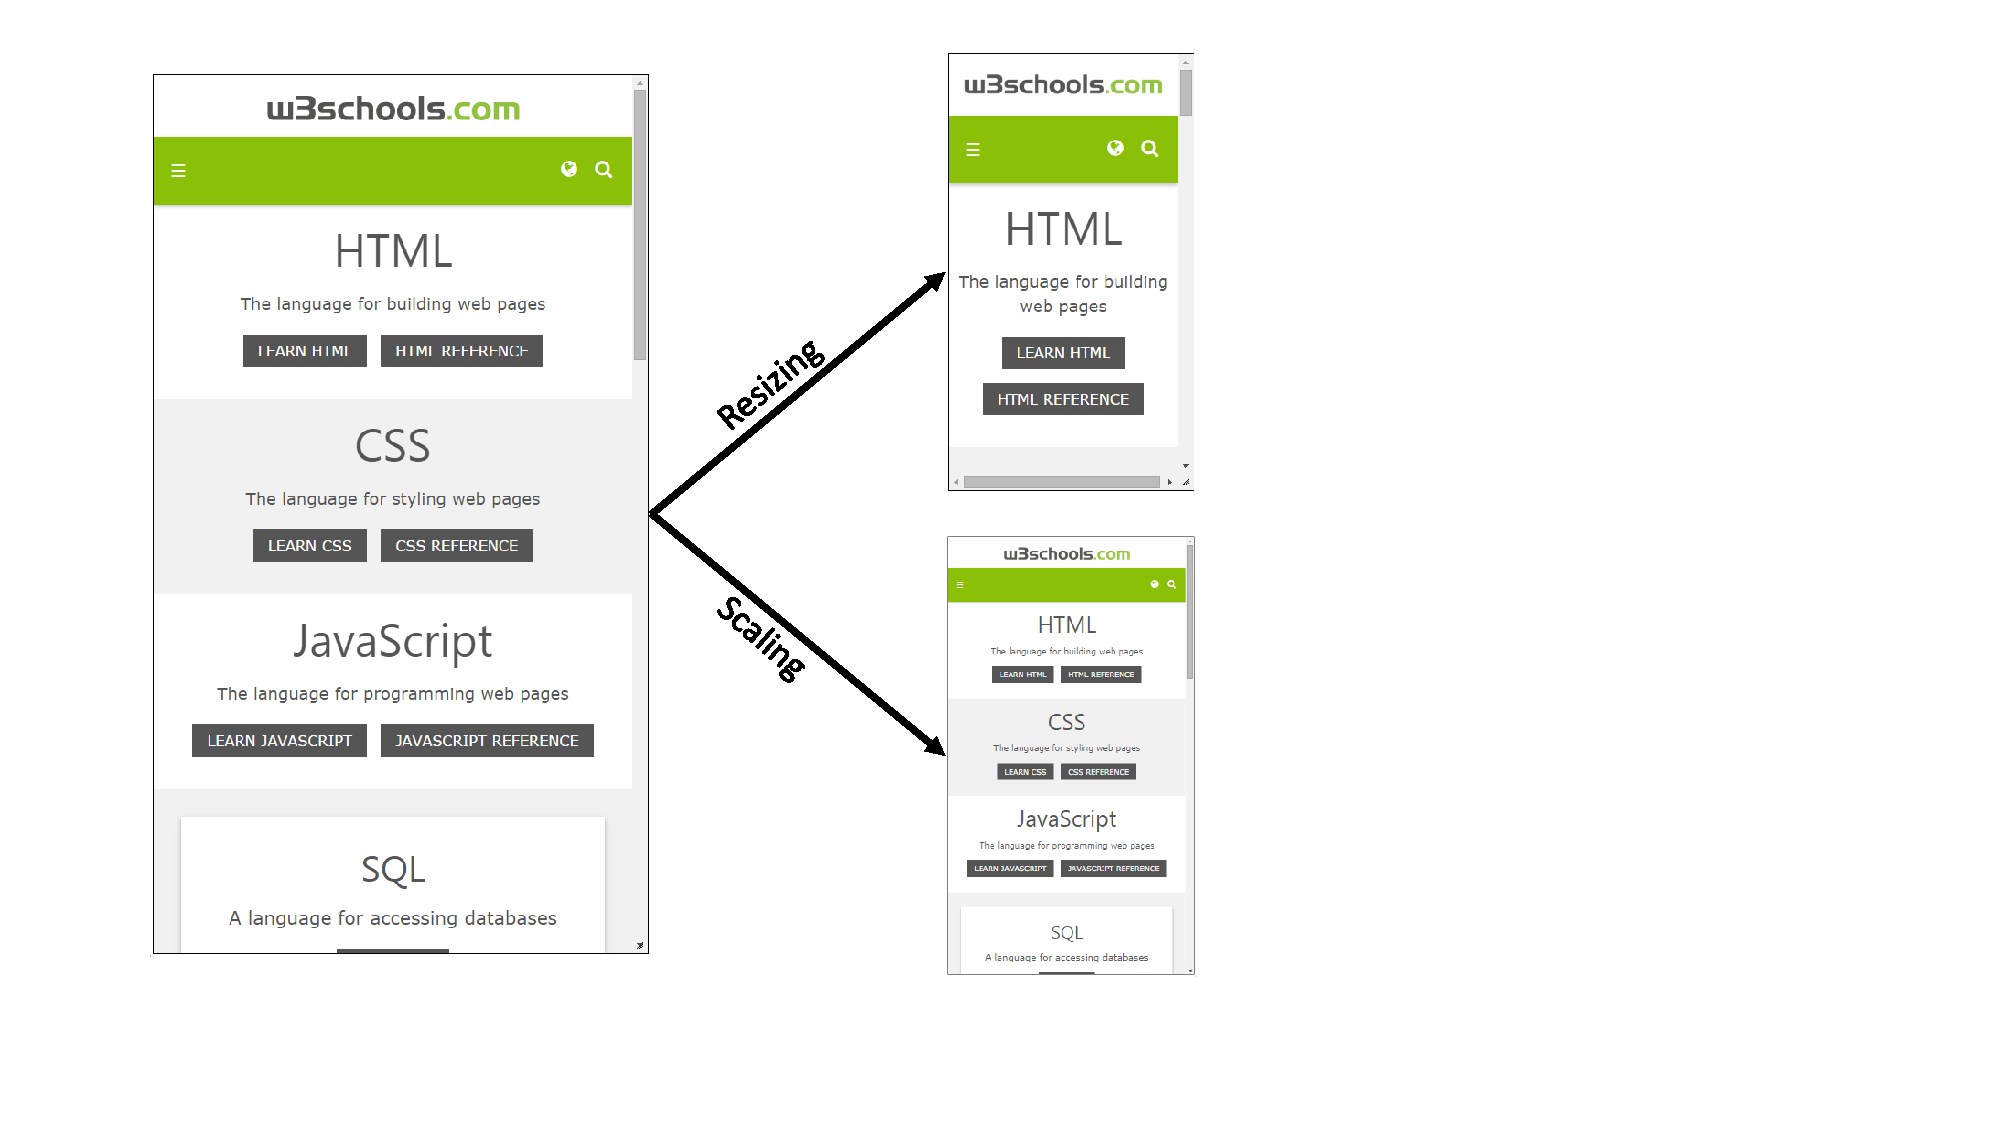
\includegraphics[width=1.0\textwidth]{images/difference_scaling_resizing.pdf}
	\caption[Difference between resizing and scaling a device]{Difference between resizing and scaling a device}
	\label{fig:difference_resizing_scaling}
\end{figure}

\section{Easy Integration of Real and Emulated Devices}

Emulating devices is a versatile tool for testing cross-device applications on many different devices. However, it does not completely eliminate the need for testing on real devices: Device emulation is always limited to certain aspects that are being emulated, e.g. screen size, resolution, touch interactions, location, and more. However, not every little detail of a real device can be emulated accurately. The following list provides an overview of some of the other limitations regarding testing on emulated devices only:
\begin{itemize}
	\item Touch interactions: Even though modern device emulators can also emulate touch interactions, performing a gesture with the mouse will never feel the same as the actual touch interaction. An interaction that works great with the mouse might feel awkward when performed on a real device and vice-versa. Also, multi-touch interactions such as pinching are difficult to emulate in a realistic way on an emulated device.
	\item Interrupts: While using an application on a real device, the user might be interrupted by things like the arriving of a text message. Those interrupts cannot be simulated in a realistic way on an emulated device.
	\item Performance: A desktop PC typically has much more computing power than a mobile device. If an application performs poorly on mobile devices, this might not even be noticed if the developer only tests on emulated devices.
	\item Display: The display quality and thus also the look of an application varies greatly depending on the device. Only emulating devices on a desktop PC cannot account for those differences in display quality. 
	\item Sensors: Modern devices have a large number of different sensors that cannot all be emulated realistically. One particular problem is the orientation of the device: A user might switch between landscape mode and portrait mode on purpose or accidentally at multiple points. Although the orientation of emulated devices can also be switched, this does not accurately simulate the behavior of a real user.
\end{itemize}
Although this list gives a good overview of the limitations of testing on emulated devices only, this list is by far not complete and what happens on a real device cannot always be foreseen by testing on emulated devices. Thus, testing on real devices is crucial for the successful development of a cross-device application. 

The importance of testing on real devices leads to a new requirement for XDTools: It should easily be possible to connect real devices to XDTools. 

\section{Easy Switching of Device Configurations}

Cross-device applications are typically used by different sets of users and thus also different devices. Even the same user may sometimes use their mobile phone and laptop simultaneously and at other times only their mobile phone or tablet. Thus, the number of devices being used with a cross-device application and those devices' characteristics may vary greatly. Depending on the devices connected to a cross-device application, the UI distribution might be different. A cross-device application needs to be able to support all those different device scenarios. However, some cross-device applications are also targeted to specific scenarios, e.g. a presentation room with multiple big screens that are always present, in addition to some mobile devices that are only in the room when their owner is attending a presentation. In such an application, the developer would probably want to emulate or connect the two static devices whenever they are testing the application and dynamically add some mobile devices. Thus, it is a key requirement for XDTools that multiple different device scenarios can quickly be created and switched to support testing a large number of different use cases for applications. 

\section{Integration with Debugging Tools}

Many of the features integrated into the debugging tools of browsers are also immensely useful for testing cross-device applications, and some might even help more when testing cross-device applications than when testing traditional web applications. However, those tools are typically limited to debugging one device at a time. We have established before that XDTools should allow emulating of multiple devices in the same browser window. While this already simplifies debugging of multiple devices simultaneously somewhat, it also introduces some additional difficulties. The messages that are logged from all emulated devices are all shown in the browser debugger tools of the same window. However, trying out some things in the console by sending commands to devices becomes more difficult. Google Chrome allows the developer to switch between different frames in the console and thus address different frames with commands, but it is not always obvious which frame corresponds to which device. Also, the developer might want to try out the same thing on multiple devices and would have to switch between multiple frames to address all devices. Furthermore, even though logging messages from all devices are displayed in the console, it is difficult to find out which device sent the message. This further complicates the debugging of cross-device applications. The same limitation applies to JavaScript errors that are shown in the console, but cannot easily be related to a device. Further limitations of the browser-included debugging tools include that navigating to the HTML of an emulated device can be rather tedious, that CSS can only be applied to one device at a time and that function breakpoints can only be added on one device at a time. Especially the last limitation can make cross-device application testing difficult because different devices have different responsibilities and not all devices might use all JavaScript functions. Consequently, adding a breakpoint inside a function on one device might not help with debugging the function at all, because the function is not even called on that device. The existence of real devices complicates things even more. By connecting the device to the desktop PC via cable, the developer gets access to remote debugging in Google Chrome. Remote debugging provides the same debugging tools as the normal debugging tools, but debugging multiple devices at the same time gets even more difficult. The remote debugging of each device is opened in a new window, thus the developer once again has to navigate between multiple windows. Also, getting an overview of all logging messages from all devices and sending commands to multiple devices becomes even more difficult. However, integrating existing debugging tools into XDTools is clearly desirable: Most of those tools have been around for quite some time and thus are already well tested and have gone through a series of improvements. Also, almost all web developers have already used those tools for extensive testing and are thus already familiar with them. However, XDTools needs to extend those tools to support debugging on multiple devices simultaneously. From all this information, we derived the following requirements for XDTools:
\begin{itemize}
	\item Logging messages should all be aggregated in one place and the device the messages originated from should be easy to identify.
	\item JavaScript errors should also be aggregated and easily identifiable.
	\item It should be possible to send JavaScript commands to multiple devices at a time. 
	\item It should be easy to inspect the HTML of a specific device.
	\item It should be possible to add CSS to multiple devices at the same time (see Figure~\ref{fig:css_aggregation}).
	\item It should be possible to add breakpoints to multiple devices simultaneously.
	\item If possible, all of the above requirements should be applied to both real and emulated devices.
\end{itemize}

\begin{figure}[H]
  \centering
    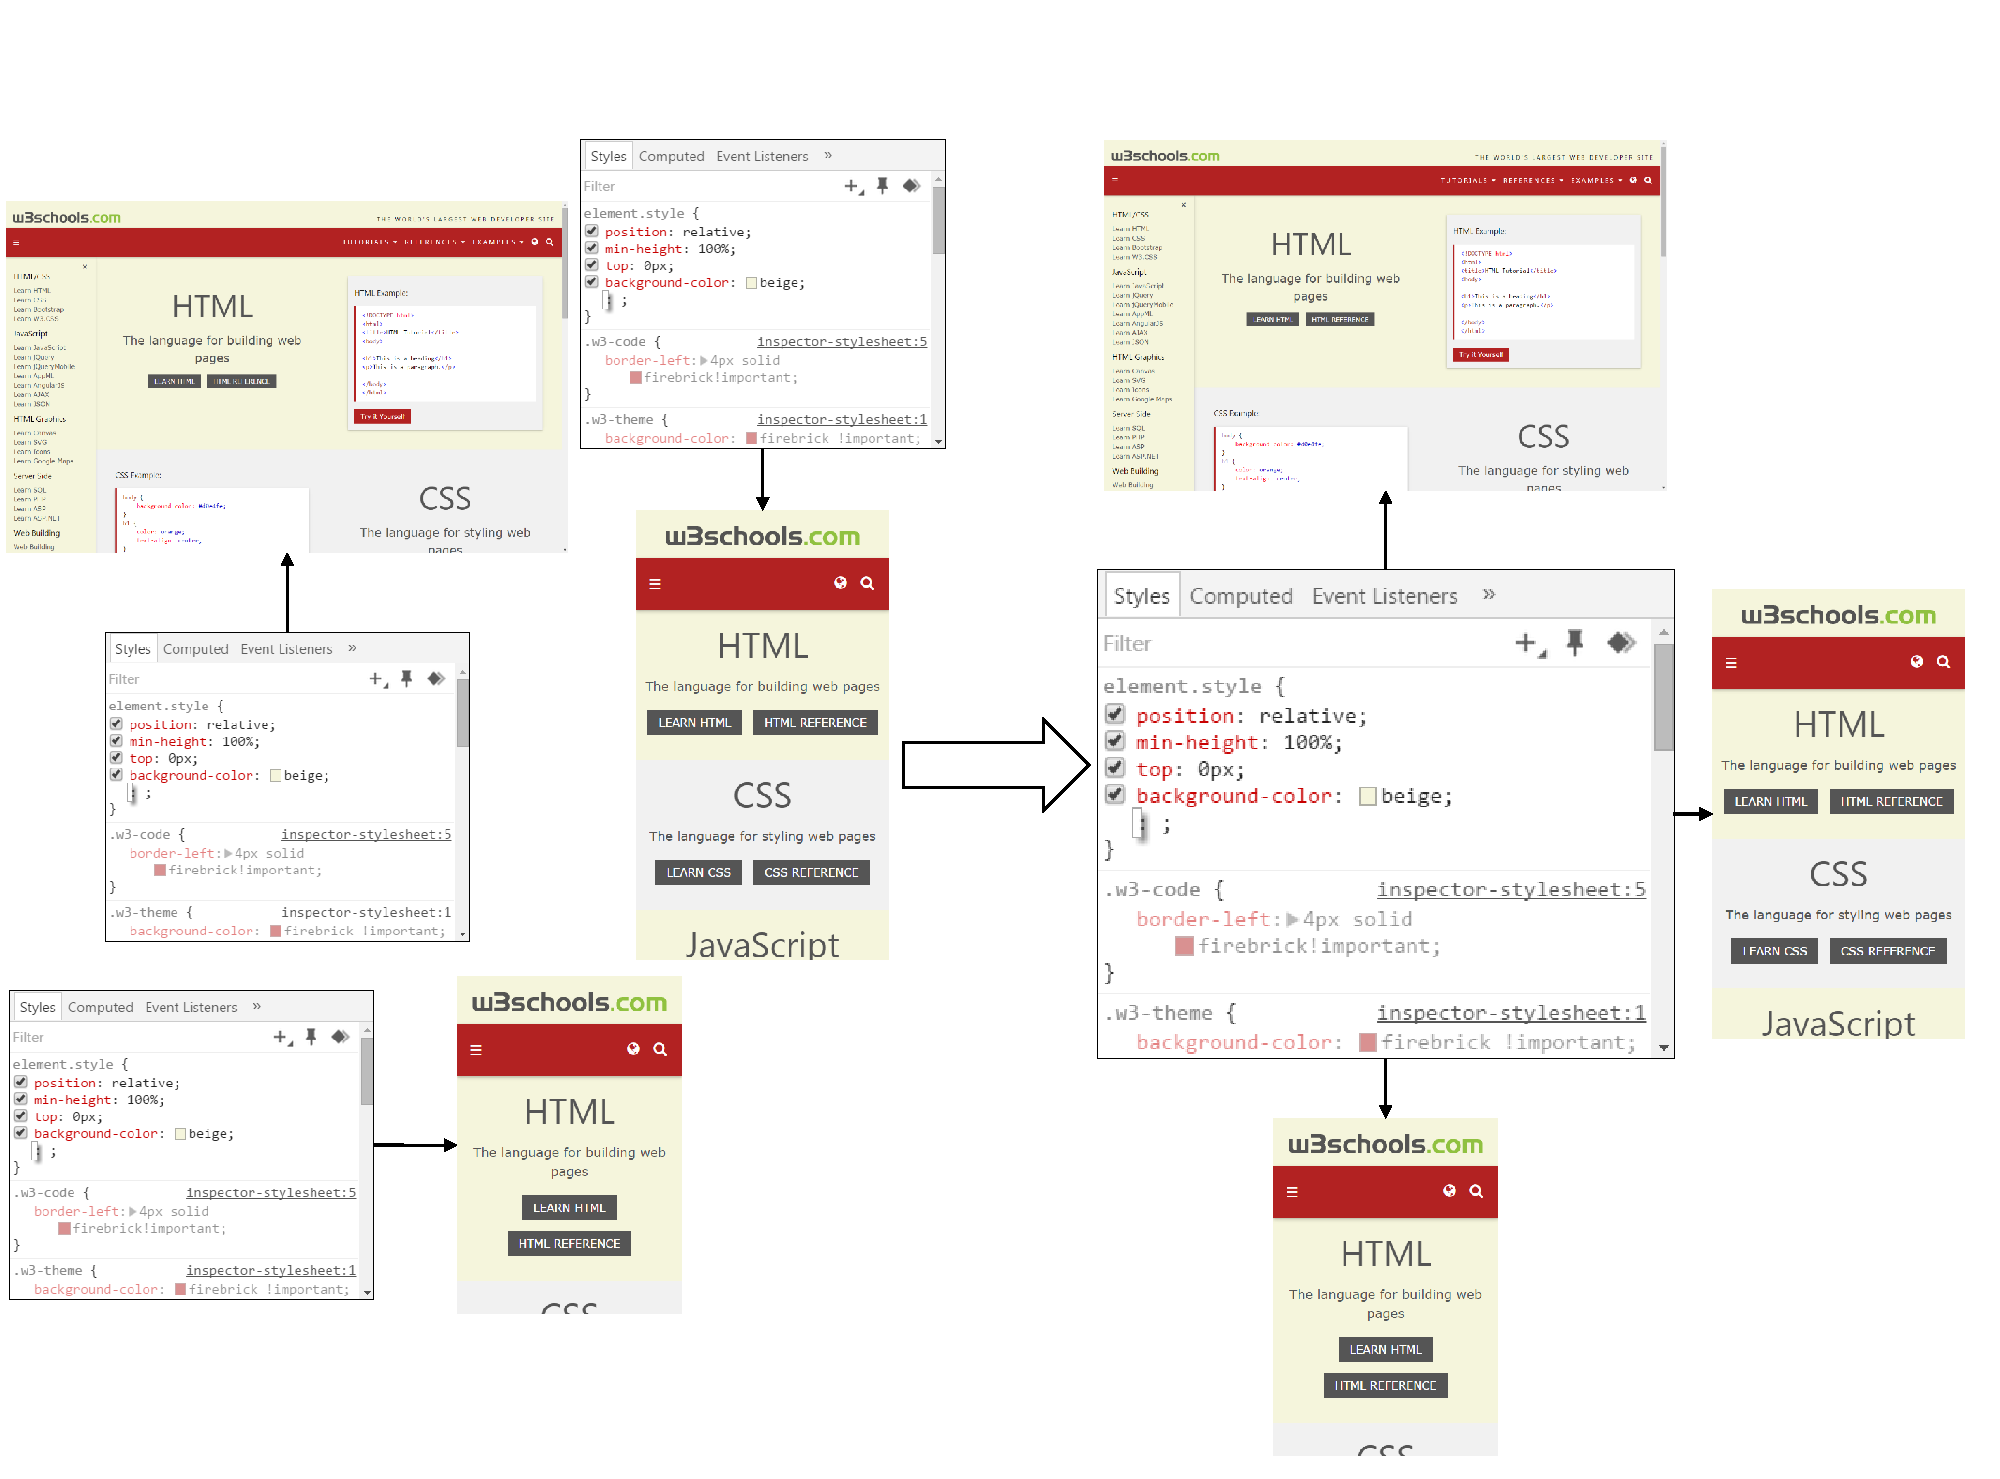
\includegraphics[width=1.0\textwidth]{images/css_aggregation_4.pdf}
	\caption[CSS editor aggregation]{CSS editor aggregation}
	\label{fig:css_aggregation}
\end{figure}

\section{Automatic Connection Management}

In order to use multiple devices in a cross-device application, those devices need to be paired with each other in some way. The mechanisms for pairing devices differ between different cross-device application frameworks: With some frameworks, all devices that open the cross-device application are paired implicitly. In other frameworks, for example XD-MVC, devices can be paired by copying the URL from one device to the other devices that should be connected. Other frameworks have more complicated mechanisms for connecting devices. In Connichiwa, one device runs a local web server and uses Bluetooth to detect nearby devices. The device then sends the IP of the web server over Bluetooth, enabling the other devices to access the received IP in a web browser. All of those three mechanisms have one thing in common: Devices are connected by opening a specific URL in the browser. However, other ways of connecting devices are also feasible: Some frameworks provide a function that can be called from a device to connect the device to another device by passing the ID of the device the device should be connected to. Also, many of the papers describing cross-device application development frameworks do not describe how devices are connected. Finally, cross-device applications can also be implemented independently of any framework and might use even more different ways for connecting devices. Thus, it is impossible to derive all ways in which devices could be connected in a cross-device application.

However, if the developer wants to debug a cross-device application, re-connecting the devices every time a new device configuration is used or possibly even when devices are refreshed is tedious and time-consuming. Thus, it is desirable to have some easy way of connecting devices. From this, we derive the next requirement for XDTools: It should be possible to automatically and manually connect devices to each other.

\section{Coordinated Record and Replay}

Record and replay has already been used previously for recording and replaying user interactions in traditional web applications and especially AJAX web applications. The non-deterministic and asynchronous nature of web applications contributes much to the value of recording and replaying interactions in web applications. When a bug is encountered during web application testing, it is often difficult to determine the exact steps for reproducing the bug. Reproducing bugs becomes even more difficult in cross-device scenarios where multiple devices are involved and the interactions performed on one device have some implications on other devices as well. Also, cross-device applications are often used by multiple users at the same time and it is difficult for the developer to simulate multiple users interacting with their devices simultaneously. Thus, we believe that record and replay can benefit cross-device application developers even more than developers of traditional web applications. However, precise mechanisms for timing replay are needed if we want to simulate multiple users simultaneously. Also, simply replaying interactions is not enough: If something goes wrong during an interaction, we need some way of pausing the replay and inspecting the state of the devices. XDTools should implement a record and replay mechanism that fulfills the following requirements:
\begin{itemize}
	\item All interactions with the device should be recorded. 
	\item It should be possible to replay a sequence of interactions on another device than the device that recorded the sequence.
	\item It should be possible to pause the replaying of the interaction sequence.
	\item Accurate timing of replays should be possible.
\end{itemize}
\chapter{XDTools}

XDTools is an integrated set of cross-device testing and debugging tools that can be loaded directly into the browser. The following sections will describe XDTools in detail.

\section{Overview of Features}

In Figure~\ref{fig:complete}, the complete interface of XDTools except for record and replay can be seen.

\begin{figure}[H]
  \centering
    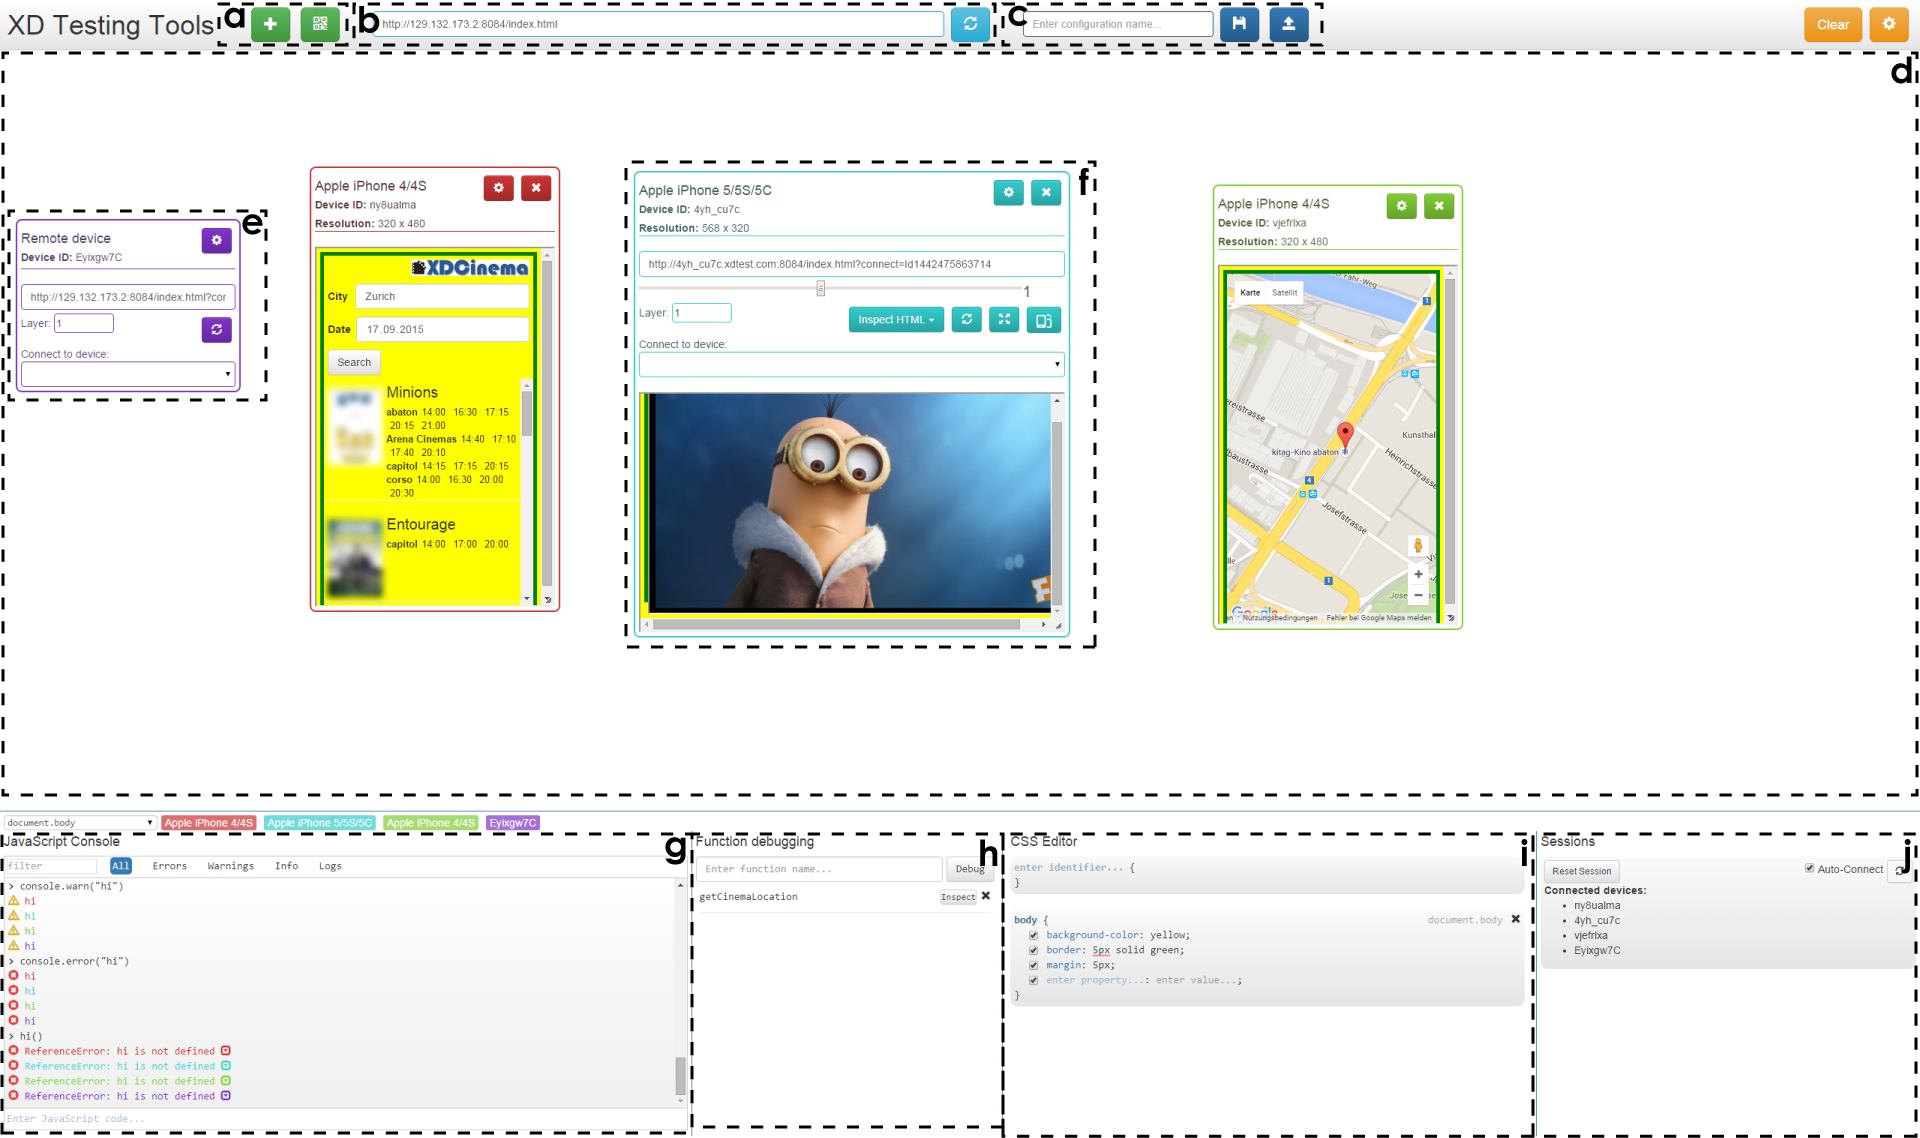
\includegraphics[width=0.95\textwidth]{images/screenshots/complete_3.png}
	\caption[Screenshot: Complete Interface]{The complete interface (without record and replay)}
	\label{fig:complete}
\end{figure}

The individual parts of XDTools are labeled in the screenshot:
\begin{itemize}
	\item [a)] Buttons for adding emulated devices and displaying the QR code that can be scanned with real devices to connect them to XDTools.
	\item [b)] Input field for loading a URL on all devices and button to refresh all devices.
	\item [c)] Loading and saving device configurations.
	\item [d)] Area where the devices can be positioned.
	\item [e)] Proxy of a connected real device.
	\item [f)] Emulated device.
	\item [g)] Shared JavaScript console.
	\item [h)] Function debugging.
	\item [i)] Shared CSS editor.
	\item [j)] Session management.
\end{itemize}

Figure~\ref{fig:complete_remote} shows a picture of the remote device that is connected to XDTools in the screenshot shown before.

\begin{figure}[H]
  \centering
    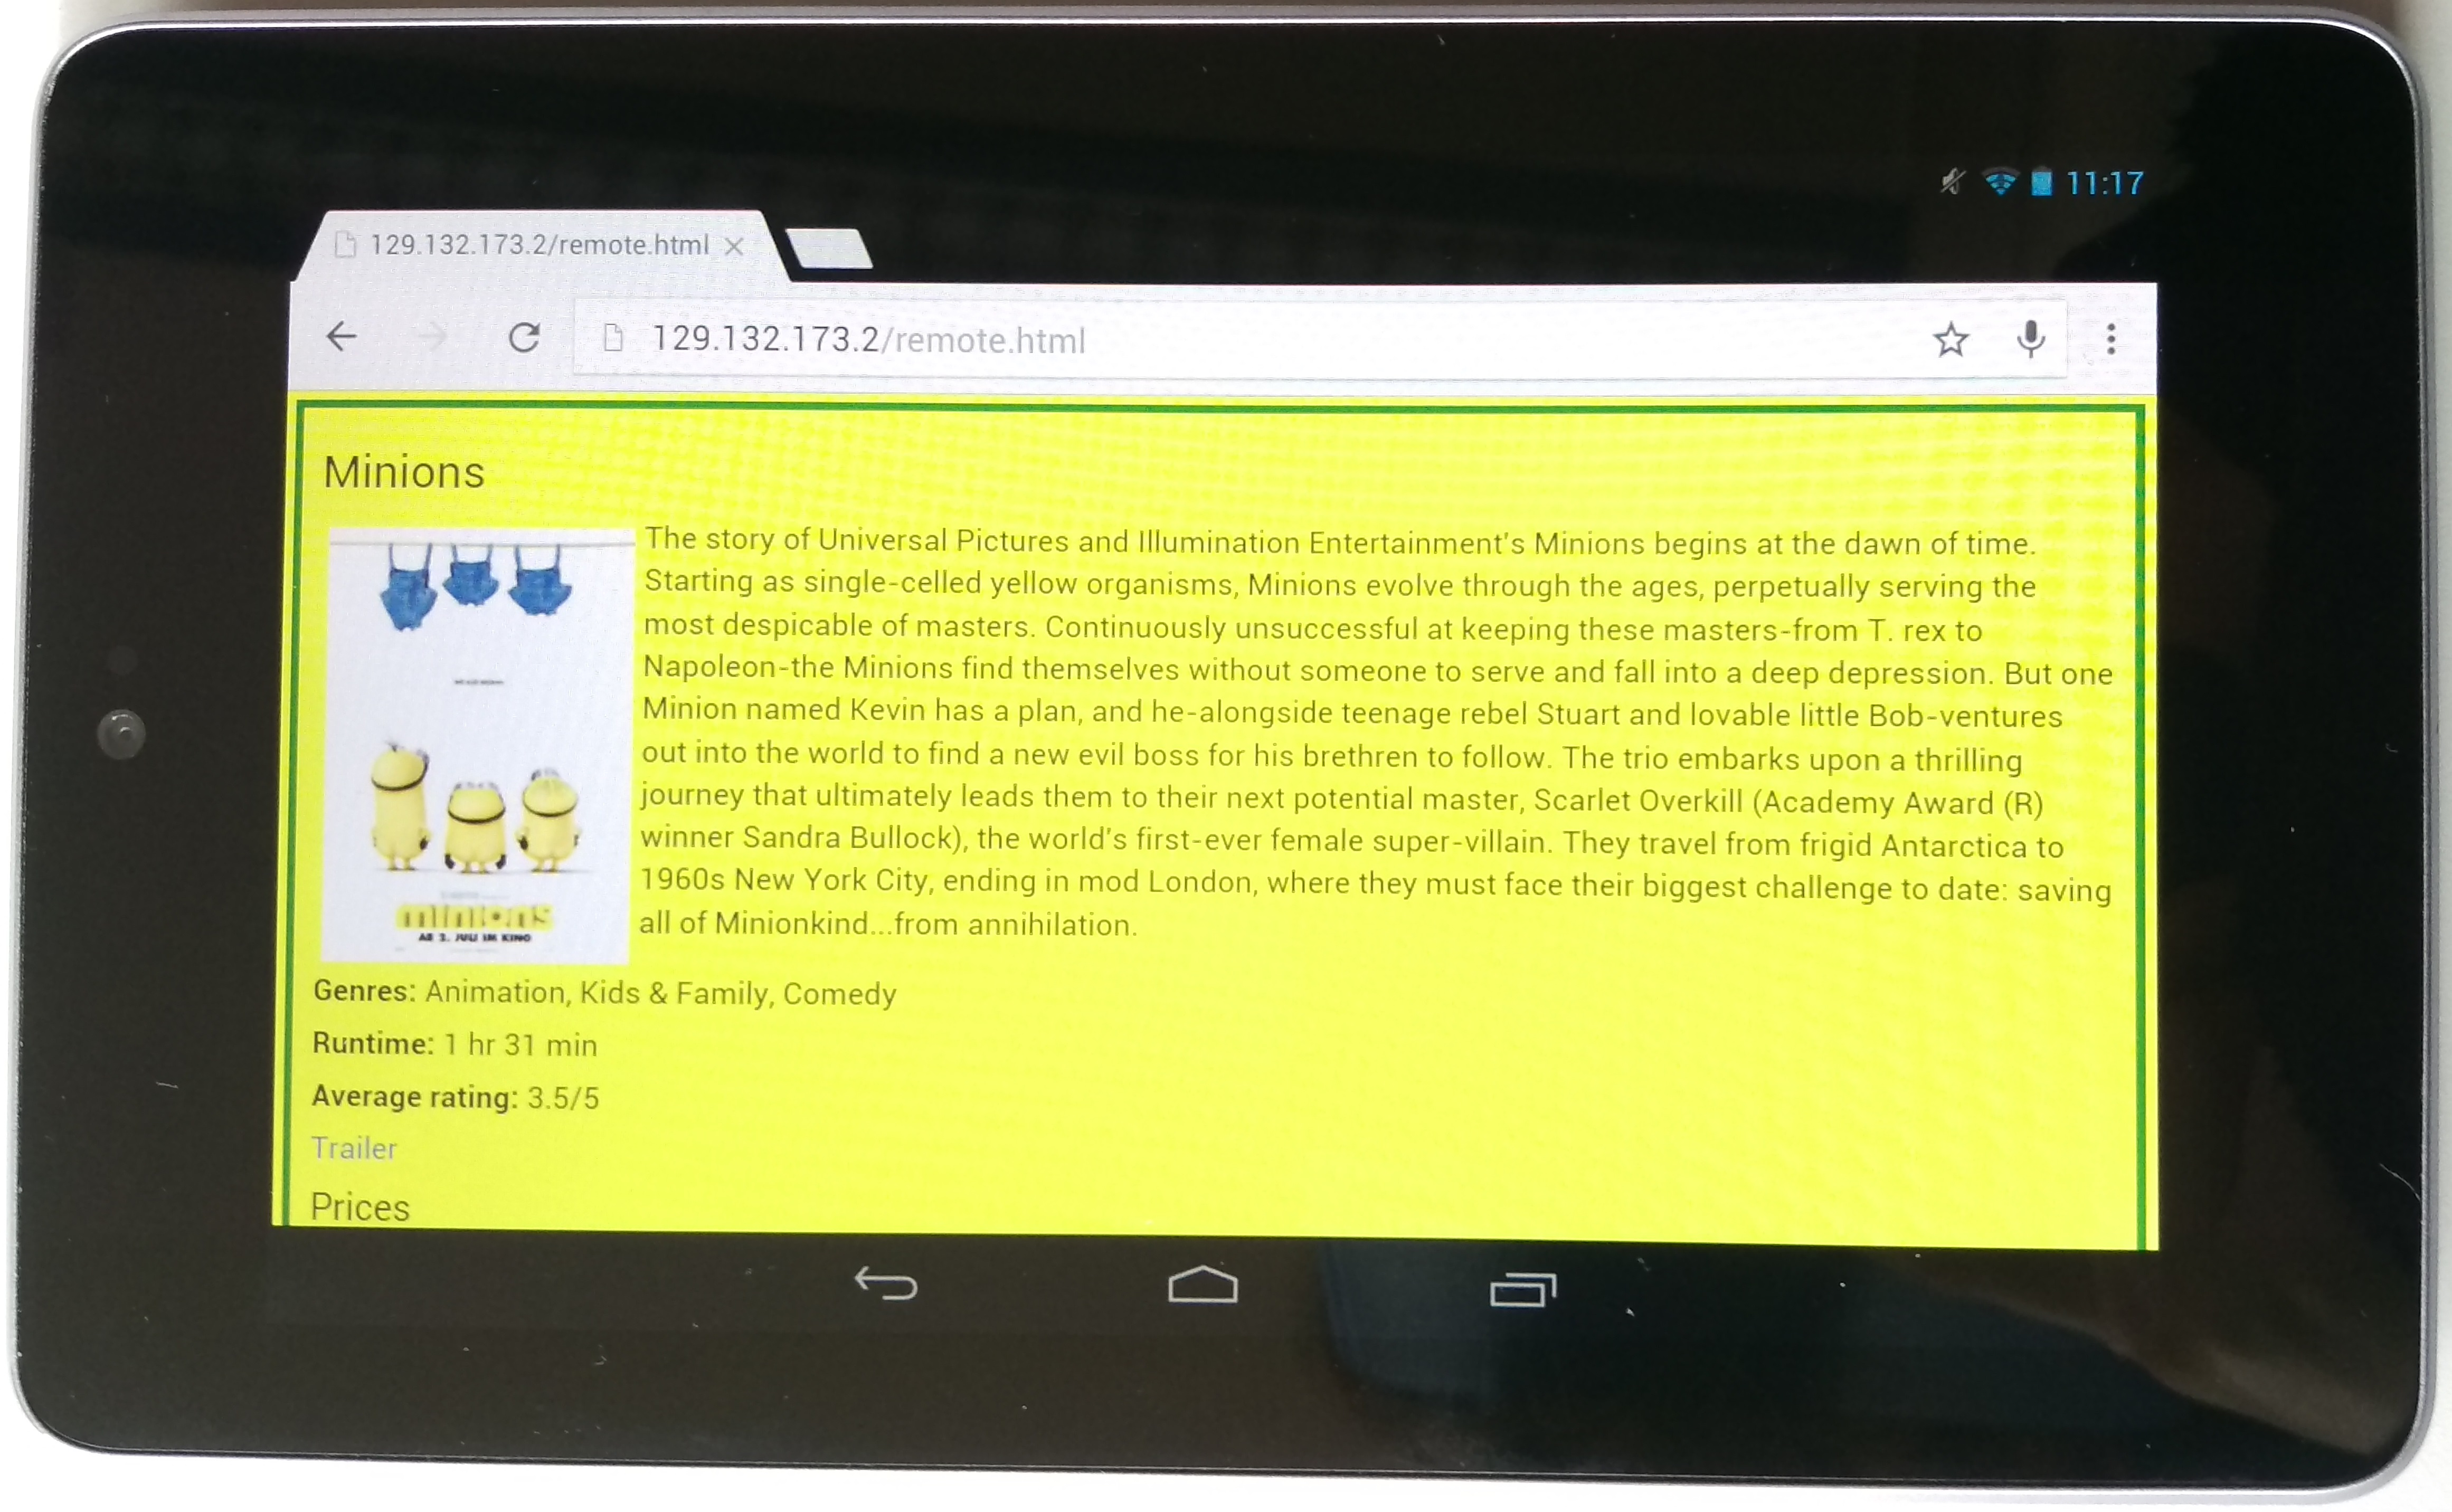
\includegraphics[width=0.95\textwidth]{images/screenshots/remote_device.jpg}
	\caption[Screenshot: Remote Device]{The connected remote device}
	\label{fig:complete_remote}
\end{figure}

XDTools also provides some options for disabling individual features, such as record and replay. If a feature is disabled, the respective interface components are simply hidden. The options also show all stored custom devices, device configurations and event sequences and allow the developer to delete any of them. A screenshot of the options can be seen in Figure~\ref{fig:options}.

\begin{figure}[H]
  \centering
    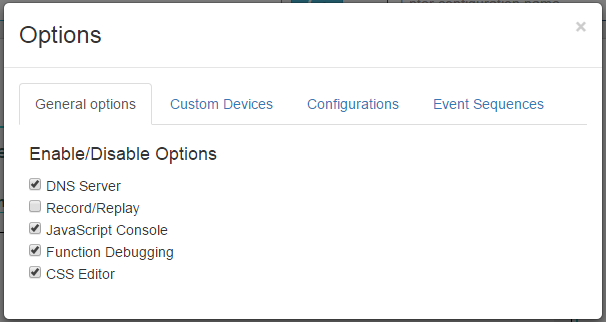
\includegraphics[width=0.75\textwidth]{images/screenshots/options.png}
	\caption[Screenshot: Options]{Options of our main application}
	\label{fig:options}
\end{figure}

Devices can be activated and deactivated by clicking on their name/ID that is displayed above the JavaScript console. When the device is active, the background of its name is in the color of the device, otherwise it is grey and the text color is in the color of the device. Figure~\ref{fig:active_inactive} illustrates the difference between active and inactive devices. The first device is inactive, the other two devices are active.

\begin{figure}[H]
  \centering
    
\includegraphics[width=0.8\textwidth]{images/screenshots/active_inactive.png}
	\caption[Screenshot: Active/inactive devices]{Active and inactive devices}
	\label{fig:active_inactive}
\end{figure}

If a device is inactive, it is not included in the following features:
\begin{itemize}
	\item Shared JavaScript console
	\item Shared CSS editor
	\item Function debugging
\end{itemize}
All those features perform some interactions with the devices automatically, thus they should ignore inactive devices. Other features like record and replay still include inactive devices because manual interaction is needed before something happens with the device. 

\section{Emulation of Multiple Devices}

XDTools allows the developer to emulate multiple devices simultaneously. The developer can either select the devices that they want to emulate from a list of existing devices or create a custom device. The developer can create a custom device just for one-time use, or they can save it to the list of existing devices for later use. This allows developers to quickly extend the devices they have access to with new devices. Devices can be assigned to one of four categories:
\begin{itemize}
	\item Desktop devices: For simplicity, this category includes all PCs, including laptops.
	\item Tablets
	\item Mobile phones
	\item Wearables
\end{itemize}
Although some devices may not easily be classified or fit into multiple categories, e.g. 2-in-1 devices that can either be used as a tablet or laptop by just plugging in a keyboard, those categories give a rough overview of the different types of devices. This categorization of devices makes it easier for developers to emulate different types of devices without having to know any exact device names. By just adding some devices from each category, the developer can make sure that a large range of devices is covered. The list of existing devices includes multiple devices from each of those categories. For the desktop devices, the list just provides some typical resolutions. The list for tablets and mobile phones includes most of the well-known devices in that area. The list of wearables so far only includes some smart watches, as most other wearables do not have access to a modern web browser (yet). Figure~\ref{fig:adding_emulated} shows the menu for adding emulated devices while the developer is adding a device from the list of predefined devices.

\begin{figure}[H]
  \centering
    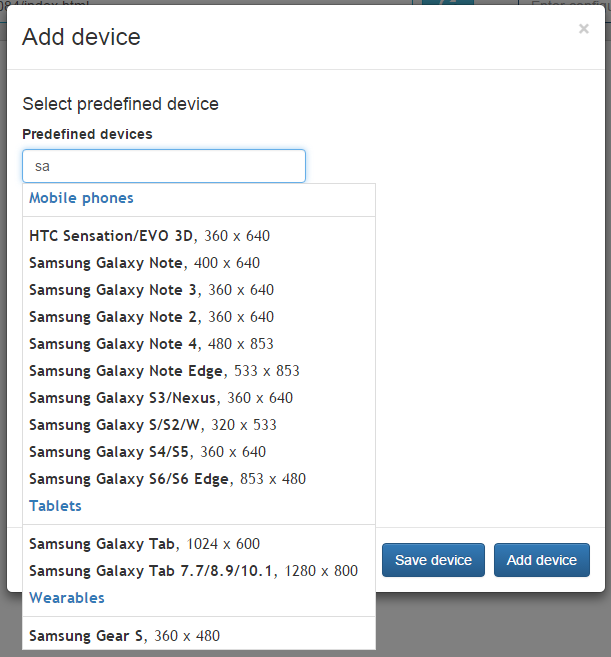
\includegraphics[width=0.75\textwidth]{images/screenshots/adding_device_predefined.png}
	\caption[Screenshot: Adding emulated devices]{Adding an emulated device}
	\label{fig:adding_emulated}
\end{figure}

Before an emulated device is created, it is assigned a unique ID. Once it is created (see Figure~\ref{fig:emulated_device}), the developer can move it to the desired location on the screen. Instead of ordering devices automatically, we decided to give the developer the freedom to choose how to order the emulated devices. This makes it easier to accurately simulate specific scenarios, e.g. a presentation room where two large screens are placed next to each other. To conquer the challenge of limited screen size, all emulated devices can be scaled up and down. Scaling a device does not change the resolution of the device and thus has no influence on the look of the application. This allows the developer to have more space available for devices. If the developer has difficulties performing an interaction on a device because it is scaled down, they can just scale it up again. However, dynamically changing the resolution of an emulated device is also possible. The developer can continuously increase or decrease the resolution of the device to immediately see what the application looks like on different resolutions. Finally, the developer can also change the layer of the device. Changing the layer of a device essentially moves the device to the front or back, thus devices can overlap each other and the developer can move the device that they want to use to the front.

\begin{figure}[H]
  \centering
    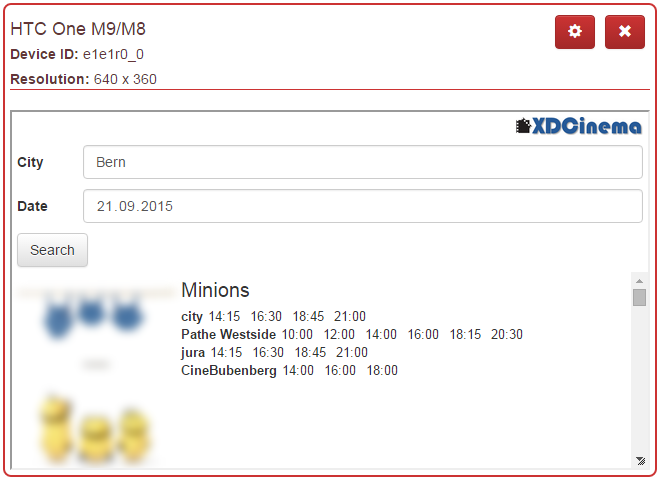
\includegraphics[width=0.8\textwidth]{images/screenshots/emulated_device_3.png}
	\caption[Screenshot: Emulated device]{An emulated device}
	\label{fig:emulated_device}
\end{figure}

Apart from its unique ID, each device also has a unique color. The border of the emulated device is colored with this color and the color is used in multiple other places for identifying the device. The devices also have a settings menu. In the settings menu, the developer can configure the following things:
\begin{itemize}
	\item The URL of the device.
	\item The scaling of the device.
	\item The orientation of the device.
	\item The layer of the device. 
	\item The device can be refreshed.
	\item The developer can inspect the HTML of the device.
	\item The developer can connect the device to another device by choosing the other device's ID from a drop-down menu.
\end{itemize}
A device's settings are not constantly used by the developer and displaying them at all times would occupy valuable screen space. Thus, the settings menu can be extended and collapsed by clicking a button. An example of a settings menu can be seen in Figure~\ref{fig:settings_menu}. 

\begin{figure}[H]
  \centering
    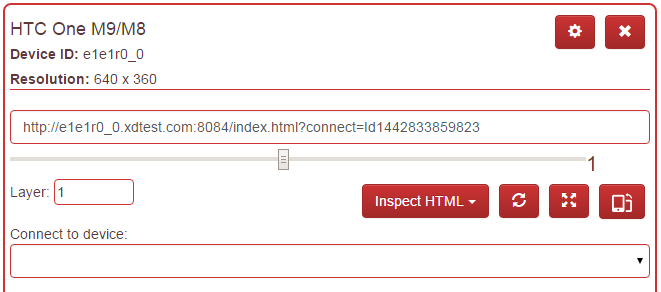
\includegraphics[width=0.8\textwidth]{images/screenshots/settings_menu_2.png}
	\caption[Screenshot: Settings menu emulated device]{Settings menu of an emulated device}
	\label{fig:settings_menu}
\end{figure}

Finally, XDTools also includes a mechanism that prevents the sharing of local resources between emulated devices.
 
\section{Easy Integration of Real and Emulated Devices}

As mentioned before, the developer should be able to connect real devices to XDTools. QR codes have become increasingly popular over the last few years and almost all devices nowadays are equipped with at least one camera. Thus, XDTools includes a QR code that can be displayed and scanned by developers to connect a real device to XDTools. As a fallback mechanism, devices can also be connected by typing a URL in the browser of the device. This makes it easy and efficient to connect a large number of real devices to XDTools. When the URL is opened, the device loads the application under test. The real devices only show the application under test and no additional interface elements. Thus, the developer can use the application on the real device, but everything related to testing and debugging is coordinated through the PC running XDTools. Each connected device is represented by a proxy within XDTools. The proxy of the real device also contains a settings menu similar to the one of an emulated device. However, the settings menu is missing a few things:
\begin{itemize}
	\item Scaling of the device: There is no need to scale real devices, as the application under test is shown on the device itself.
	\item Switching orientation: The orientation of a real device can be switched on the real device itself by simply rotating the real device.
	\item Inspecting the HTML: The developer's PC has no access to the HTML of the real device, thus it cannot be inspected.
\end{itemize}
Figure~\ref{fig:settings_menu_remote} shows the settings menu of a remote device. The settings menu only contains the interface elements for setting the URL of the device, refreshing the device, changing the layer of the device and connecting the device to other devices.

\begin{figure}[H]
  \centering
    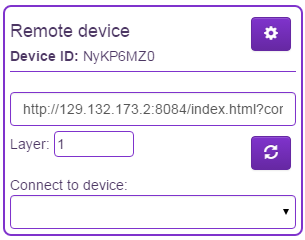
\includegraphics[width=0.5\textwidth]{images/screenshots/remote_device.png}
	\caption[Screenshot: Settings menu remote device]{Settings menu of a remote device}
	\label{fig:settings_menu_remote}
\end{figure}

The proxy of the real device can be moved around just like the emulated devices and its settings menu can also be collapsed and extended. Furthermore, each real device also has a unique ID and color for easy identification.

The developer can use emulated devices alongside real devices. Thus, XDTools allows the developer to test their application on only emulated devices, only real devices, or both at the same time. This flexibility makes it easy to test a large number of different scenarios.

\section{Easy Switching of Device Configurations}

XDTools allows the developer to create some emulated devices, save this device configuration for later, and then re-use it. For each emulated device in a device configuration, the following information is stored:
\begin{itemize}
	\item Its ID.
	\item Its resolution.
	\item Its position.
	\item Its scaling.
	\item Its layer.
\end{itemize}
Storing device configurations makes it easy for the developer to re-use device configurations and switch between different device configurations efficiently. Thus, testing a cross-device application with many different device scenarios can be done without much effort. A user can just load one device configuration, try out the application and switch to the next device configuration if everything works as expected. The developer can also create a device configuration where only static devices used with the application under test are saved in the configuration and dynamically add more devices.

If the developer wants to save a device configuration, they can type the name of the device configuration into an input field and then click the save button to save the current device configuration under that name. If they want to load a device configuration instead, they can type its name into the same input field and click the load button to load the device configuration with that name (if it exists). Autocompletion is used for providing suggestions for device configurations that could be loaded (see Figure~\ref{fig:session_management}). 

\begin{figure}[H]
  \centering
    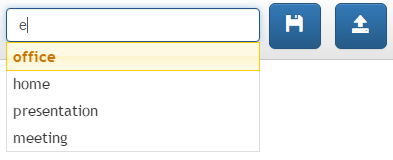
\includegraphics[width=0.6\textwidth]{images/screenshots/session_management_2.png}
	\caption[Screenshot: Saving/Loading device configurations]{Saving/Loading Device Configurations}
	\label{fig:session_management}
\end{figure}

\section{Integration with Debugging Tools}

In the previous chapter, we described the requirements for a tight integration of XDTools with some of the most useful browser debugging tools. In the following, we will describe how the integration of the debugging tools is realized in XDTools.

\subsection{Shared JavaScript Console}

XDTools includes a JavaScript console that is shared between all emulated and real devices. Each emulated and real device forwards all logging messages to the console which then aggregates these messages. Each message is displayed in the color of the device that it was sent from. This color-coding makes it trivial to identify the device a message originated from. Apart from forwarding logging messages, the devices also forward their JavaScript errors. Whenever a JavaScript error occurs, the JavaScript error message is sent to the console, together with the stack trace if available. When a JavaScript error with stack trace is received by the console, the stack trace is split into multiple lines where each line represents one entry of the stack trace. By default, the developer only sees the error message itself without the stack trace. By clicking on a button next to the error message, the developer can extend and collapse the stack trace. Figure~\ref{fig:stack_trace} shows what such a stack trace looks like in the JavaScript console.

\begin{figure}[H]
  \centering
    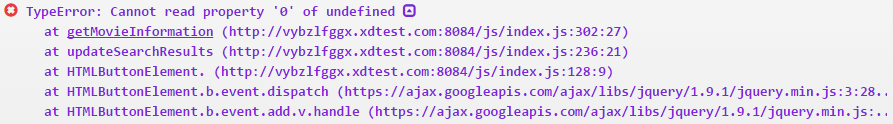
\includegraphics[width=1.0\textwidth]{images/screenshots/stack_trace_4.png}
	\caption[Screenshot: Stack trace]{Stack trace}
	\label{fig:stack_trace}
\end{figure}

For easier identification of the type of a message, all messages are assigned to one of four categories:
\begin{itemize}
	\item Warnings: This includes all warning logging messages.
	\item Errors: This includes all error logging messages and JavaScript errors.
	\item Info: This includes all info logging messages.
	\item Log: This includes all other types of messages.
\end{itemize}
Depending on the type of message, a different symbol is used in front of the message when it is displayed in the shared JavaScript console. This makes it easy to see if a message is an error or just a simple logging message.

Due to the aggregation of multiple devices, a large number of messages is displayed in the console, making it difficult to look for a specific message. To solve this problem, the messages in the console can be filtered by the type of message, e.g. show only error messages, or by text. If the console messages are filtered by text, all messages that do not contain the text to filter by anywhere are hidden. If the filter is removed, the hidden messages are shown again. If a device is deactivated, it does not forward any messages or errors anymore and all existing messages are filtered out until the device is activated again. 

The console also allows sending commands to multiple devices. If the developer wants to send a command to the devices, they can type the command into an input field below the console and press the enter key. The developer can either send the command to all devices or they can deactivate some devices and only send the message to a subset of devices. Being able to send a command only to a subset of devices is important in a cross-device setting because some commands might only make sense on some devices and executing them on all devices could lead to potential errors or a decrease in performance. The return values of commands are also displayed in the console, again color-coded to match the device they came from. Thus, otherwise time-consuming tasks like checking the value of a global variable on all devices become trivial. The console works exactly the same for emulated and real devices. This aggregation of console outputs from both emulated and real devices at least partially eliminates the need for remote debugging.

The shared JavaScript console also has a history function similar to the console in Chrome DevTools. By using the arrow keys, the developer can navigate through the history and call previous commands again.

The screenshot in Figure~\ref{fig:js_console} shows the shared JavaScript console including a few examples of how to use it. First, the developer tries to call a function but makes a typo. Because the function with the typo in the name does not exist, an error message is displayed by all devices. The developer then notices the typo, types the correct function and sees the return values of the function (the coordinates of a cinema). Finally, the developer wants to see which roles have been assigned to the devices. They type the name of the variable that stores the roles and the value of this variable is shown in the console.

\begin{figure}[H]
  \centering
    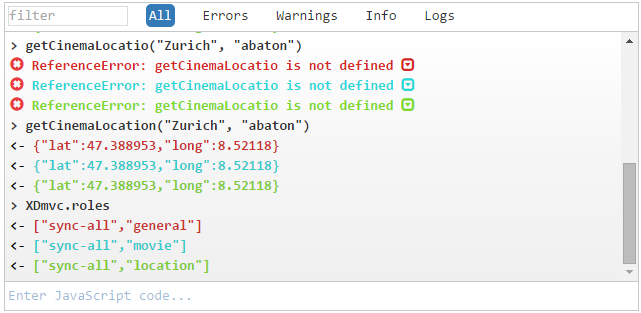
\includegraphics[width=1.0\textwidth]{images/screenshots/js_console_3.png}
	\caption[Screenshot: JavaScript console]{Shared JavaScript console}
	\label{fig:js_console}
\end{figure}

\subsection{Function Debugging and Inspection}

Function debugging allows developers to debug a function on multiple emulated devices without having to add breakpoints on each device individually.

If the developer opens the Chrome DevTools, an additional area at the bottom of XDTools appears. In this area, the developer has access to an input field where they can type the name of a function that they want to debug. Below the input field, the list of functions that are currently being debugged is shown. Whenever one of the debugged functions is called on any device, the debugger pauses at the beginning of the function and the developer can perform their debugging actions. The device on which the function is called is highlighted until the function call returns, making it easy to identify the device that is currently being debugged.

Figure~\ref{fig:function_debugging_complete} shows a screenshot while a function is being debugged. The screenshot shows the highlighted device, the Chrome DevTools with the source code of the debugged function and the list of debugged functions.

\begin{figure}[H]
  \centering
    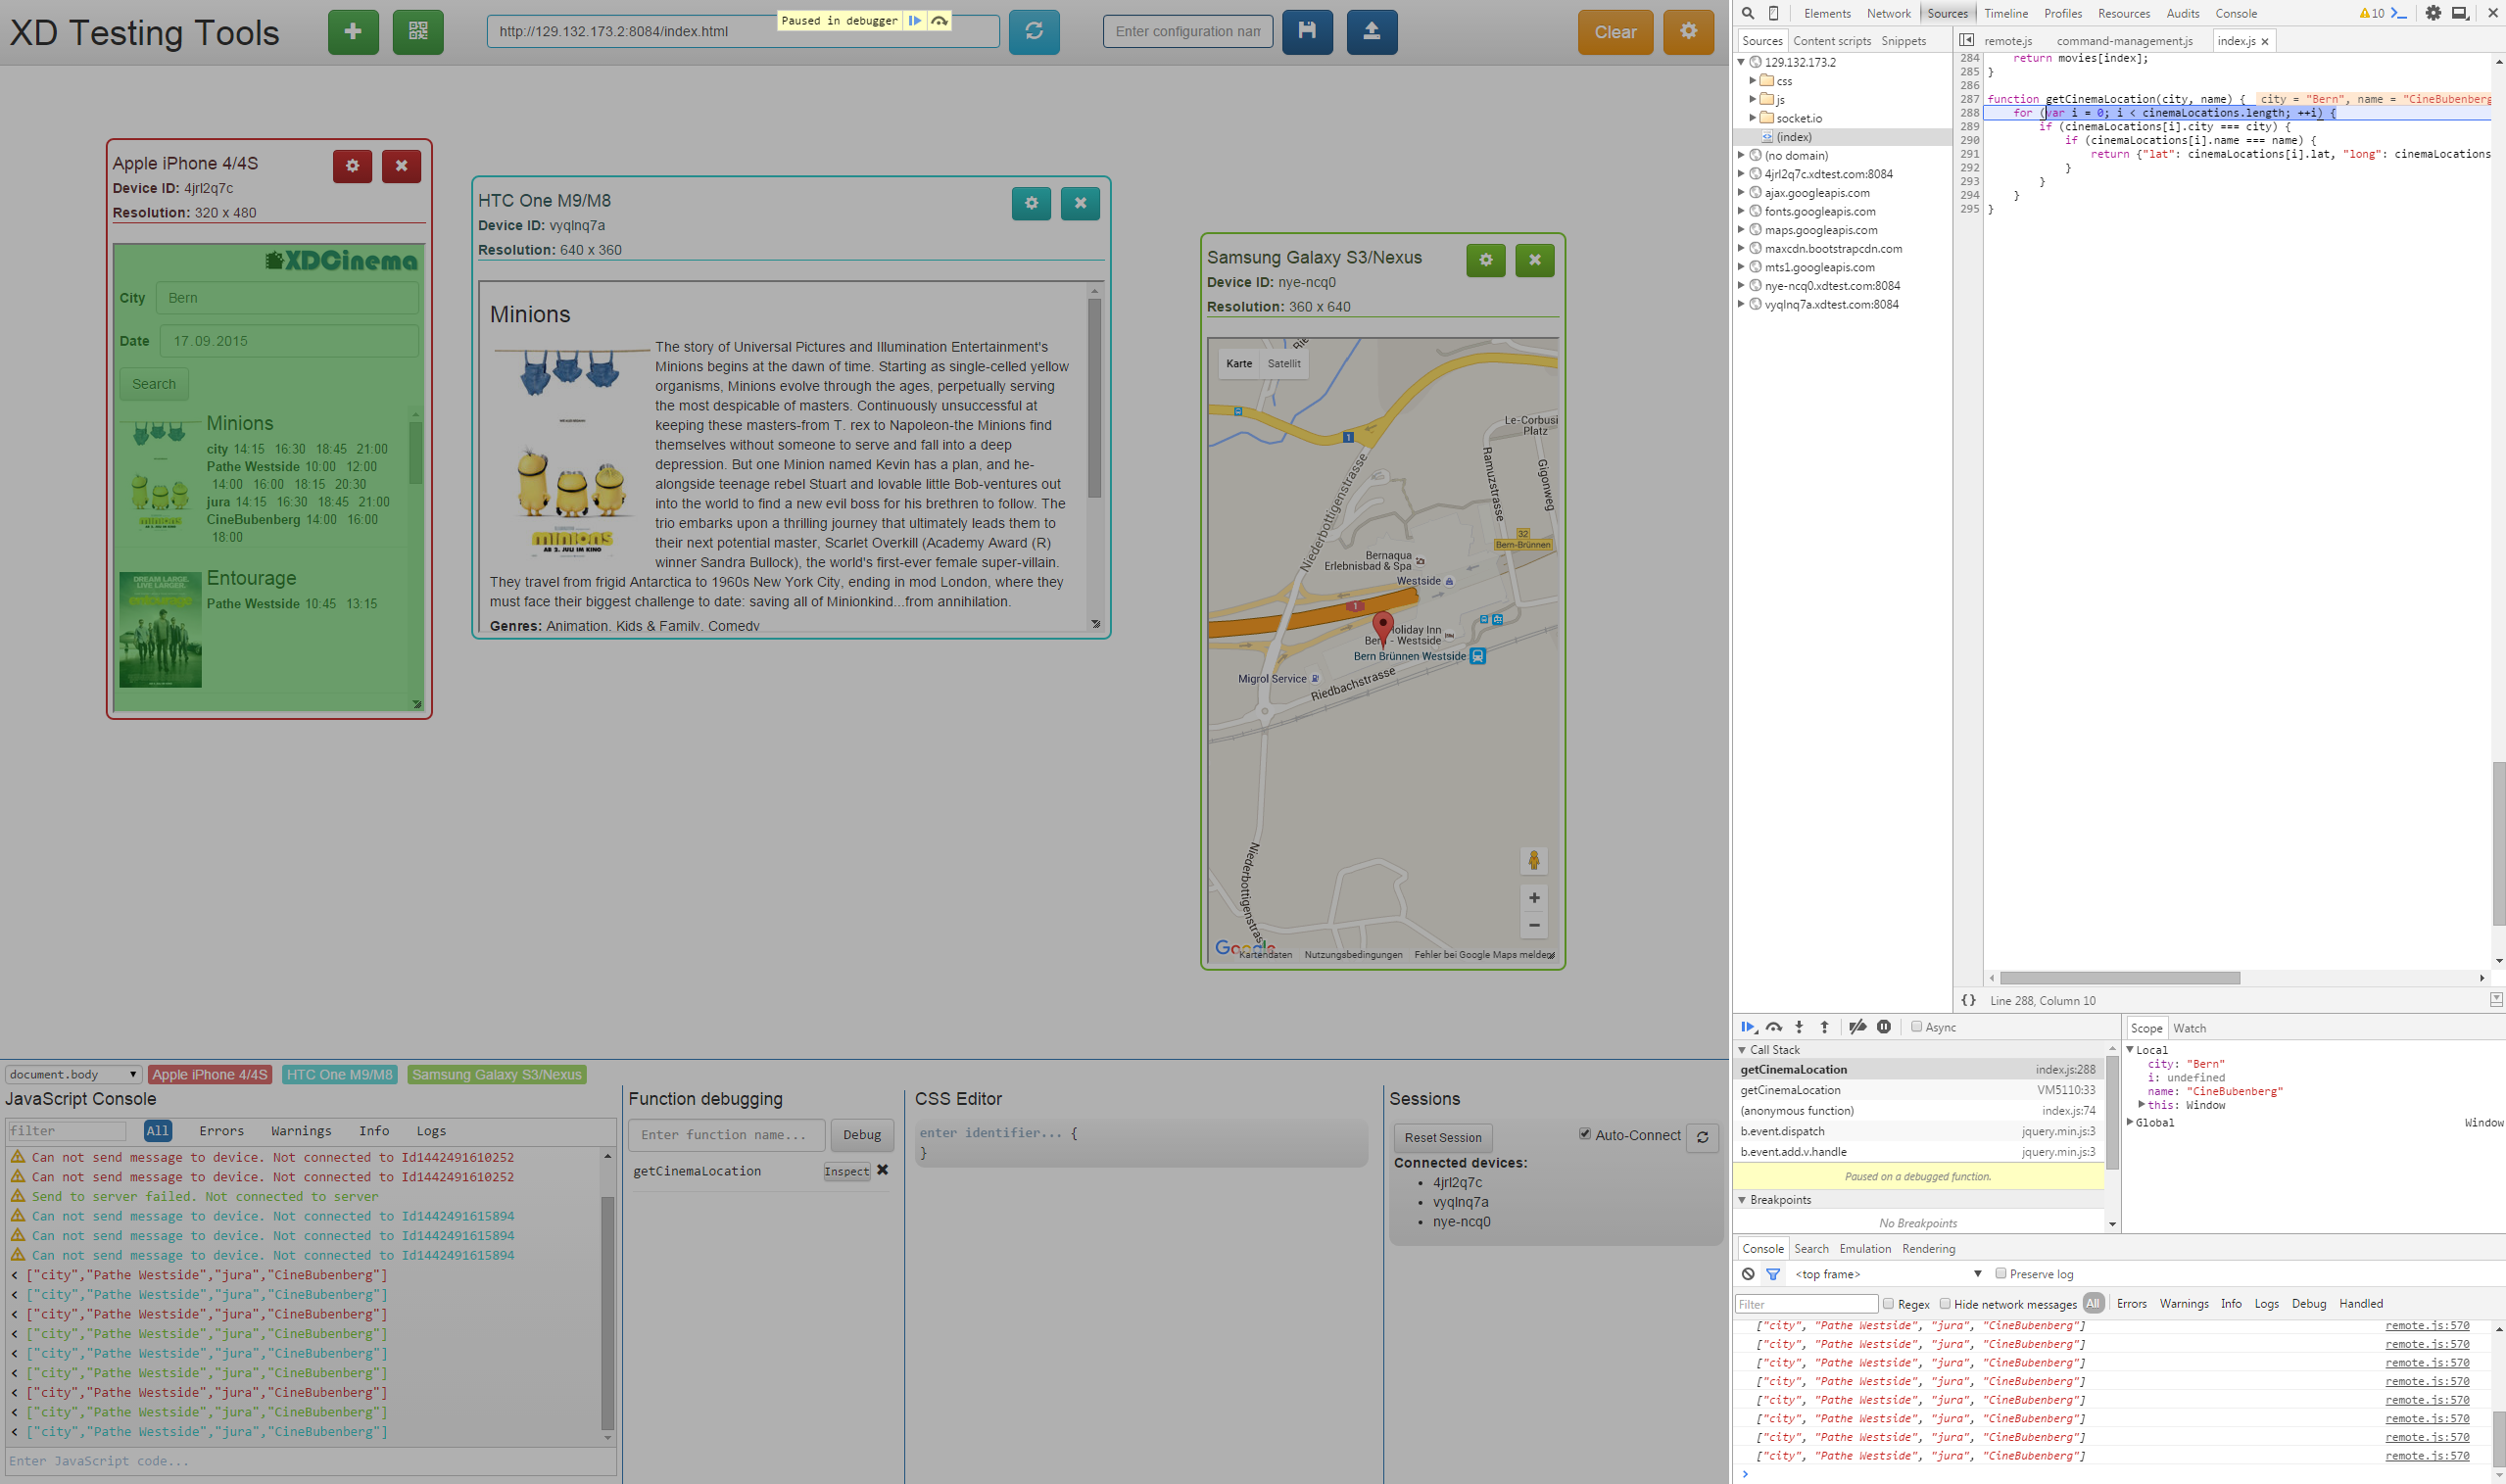
\includegraphics[width=1.0\textwidth]{images/screenshots/function_debugging_complete.png}
	\caption[Screenshot: Function debugging]{The complete interface while debugging a function}
	\label{fig:function_debugging_complete}
\end{figure}

If the developer is done debugging a function, they can remove it from the list of debugged functions.

The developer can also just inspect the source code of the function without it being called by clicking on a button next to the function name in the list of debugged functions. If this button is clicked, an emulated device is picked at random and the source code of the function is opened on this device. 

Unfortunately, function debugging only works on emulated devices. Chrome's DevTools do not have access to the JavaScript code of a connected real device, thus debugging the function using the DevTools is impossible without remote debugging.

\subsection{HTML Inspection}

XDTools allows the developer to directly jump into the HTML of an emulated device. Inside the settings menu of each emulated device, a button can be clicked to inspect the HTML of the device. Clicking this button opens the \lstinline|body| element of the device in the Chrome DevTools. 

HTML inspection is only available on emulated devices for the same reasons that we already mentioned before.

\subsection{Shared CSS Editor}

XDTools also includes a custom CSS editor. The CSS editor is designed to feel similar to the CSS editors typically provided by browsers. The developer can specify a selector and then add some rules that are applied to HTML elements that match the selector. The CSS rules are applied to all active devices, including both real and emulated devices. All CSS rules can be deactivated and activated again, edited, or removed completely. This allows the developer to quickly change the CSS of multiple devices and immediately see the result. This is considerably less effort than adding rules to all devices individually or editing the CSS file, saving it and reloading all devices.

The CSS editor also has some autocomplete functionality: If the developer starts typing the name of a property, the property is automatically completed using the first CSS property name that matches the text typed by the developer (see Figure~\ref{fig:css_autocomplete}).

\begin{figure}[H]
  \centering
    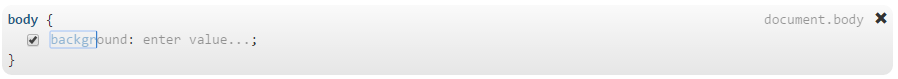
\includegraphics[width=1.0\textwidth]{images/screenshots/css_autocomplete.png}
	\caption[Screenshot: CSS editor autocompletion]{Autocompletion in the CSS editor}
	\label{fig:css_autocomplete}
\end{figure}

Figure~\ref{fig:css_editor} shows a screenshot of the CSS editor in action. In this screenshot, some CSS rules are added to the \lstinline|body| element of all devices.

\begin{figure}[H]
  \centering
    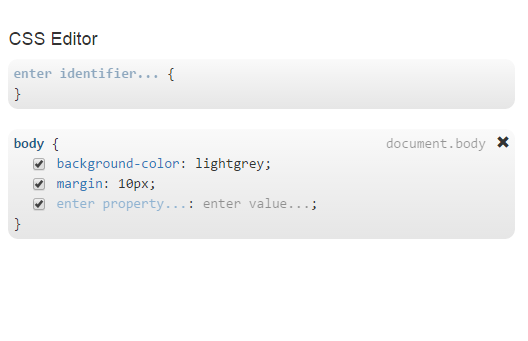
\includegraphics[width=1.0\textwidth]{images/screenshots/css_editor.png}
	\caption[Screenshot: CSS editor]{Shared CSS Editor}
	\label{fig:css_editor}
\end{figure}

In Figure~\ref{fig:css_applied}, the effects of the CSS shown in the screenshot before are shown. 

\begin{figure}[H]
  \centering
    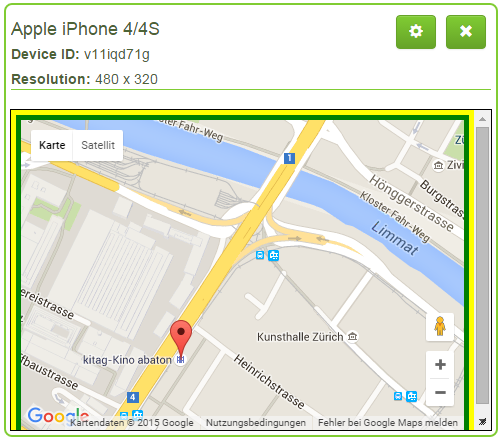
\includegraphics[width=0.5\textwidth]{images/screenshots/emulated_device_4.png}
	\caption[Screenshot: CSS effects]{CSS applied to emulated device}
	\label{fig:css_applied}
\end{figure}

\section{Automatic Connection Management}

The devices in XDTools can either be connected automatically or manually. Each set of connected devices represents a session. For each session, a checkbox allows the developer to toggle on or off auto-connect. When the first device is created or connected, auto-connect is switched on by default. If auto-connect is on, all newly created and connected devices will automatically be connected to that session. Thus, if the developer simply adds or connects a number of devices, they will automatically all be connected. If the developer wants to have multiple sessions, they can turn off auto-connect and then add more devices. Each device also has a drop-down menu in its settings menu for manually connecting to other devices. Only one session can have auto-connect enabled; if the developer switches on auto-connect for one session, it is switched off for all other sessions.

All current sessions are displayed at the bottom of XDTools. Each session displays all connected devices (see Figure~\ref{fig:sessions}). The developer can also refresh all devices in a session or reset a session. Resetting a session assigns new IDs to all devices and thus erases the local resources of the devices. 

\begin{figure}[H]
  \centering
    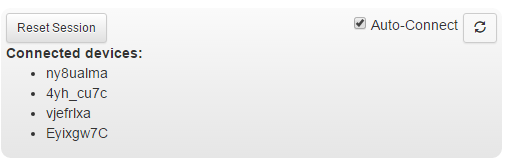
\includegraphics[width=0.6\textwidth]{images/screenshots/session_management.png}
	\caption[Screenshot: Session]{A device session}
	\label{fig:sessions}
\end{figure}

So far, automatic connection is only possible for applications that connect via URL. However, the URL required for connecting depends on the application under test. XDTools provides a custom connection function that can be adjusted by the developer such that it returns the appropriate URL.

\section{Coordinated Record and Replay}

XDTools allows the developer to record a sequence of interactions on a device and replay it. Recording can be started on a device at any time. Once recording has started, the developer can perform the desired interactions on the device. After a device finishes recording, the event sequence is visualized (Figure~\ref{fig:record_replay}). The interactions can then be replayed on the same device, moved to other devices, or saved for later.  Furthermore, event sequences can be cut into multiple parts. The timing of the replays can be configured arbitrarily by dragging and dropping event sequences. This allows the developer to configure replays in many different ways: They can be executed in parallel, one after another, or anything in-between. The replays can be started on all devices simultaneously or on one device at a time. This makes it easy to simulate multiple users and devices. Since the events in an event sequence are performed by a real user, i.e. the developer, the timing of the individual events in an event sequence is very realistic.

\begin{figure}[H]
  \centering
    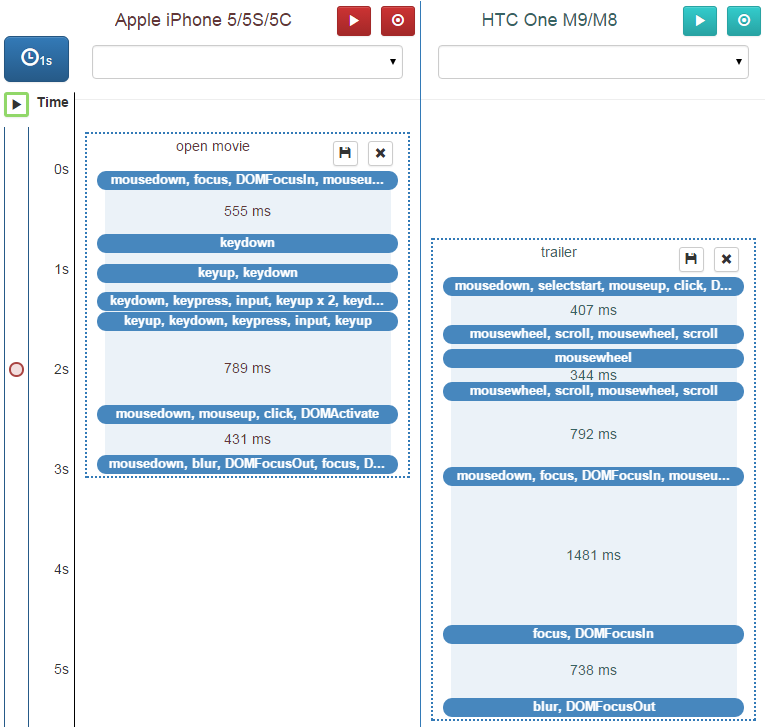
\includegraphics[width=1.0\textwidth]{images/screenshots/record_replay_2.png}
	\caption[Screenshot: Record and replay]{Record and Replay}
	\label{fig:record_replay}
\end{figure}

The developer can also add breakpoints to the replay. Next to the event visualizations, a timeline is shown as well as a narrow column where the developer can click to add a breakpoint at a certain point in time. As soon as all events that occur before this point of time have been replayed, the replay pauses and the developer can inspect the state of the devices. If a breakpoint is reached, it is highlighted. After the developer chooses to continue, replay is continued until the next breakpoint is reached. After the last breakpoint has been reached, the replay continues until all events have been replayed. The developer can also add breaks of one second between events to delay all following events by clicking on a button and dragging the mouse to the place where the break should be inserted. This allows the developer to spend some more time looking at the application under test before the replay continues without having to set breakpoints. 
\section{Architecture}

\section{Choice of Technologies}

\section{General Features}

\section{Device Emulation}

\section{Connecting Real Devices}

\section{Shared JavaScript Console}

\section{Function Debugging}

\section{Shared CSS Editor}

\section{Record/Replay}
\chapter{Sample Applications}

Over the course of our project, we developed two sample applications, XDCinema and XDYouTube. While developing those applications, we used XDTools to test and debug them. Using XDTools while developing two real cross-device applications helped us gain further ideas for improving XDTools and served as a first evaluation step for XDTools. In the following, we describe the two sample applications and the insights we gained from them.

\section{XDCinema}

As the name suggests, XDCinema is a cross-device cinema application. It allows users to check the cinema listings and view different information about movies and cinemas. It can be used with one to four different devices. On the "main device", the user can specify a city and date. They will then see a list of movies that are shown in this city on that date. The application is essentially split into four different views that can be seen in Figure~\ref{fig:xdcinema} and that all show different information:
\begin{itemize}
	\item The search view (a): In the search view, the movies shown in the selected city on the selected date are shown. For each movie, the cinemas in the selected city that show the movie and the times at which the movie is shown are displayed.
	\item The location view (b): In the location view, the location of the selected cinema is shown on a map. The location view is shown when the user clicks on a cinema in the search view.
	\item The movie view (c): In the movie view, information about the selected movie is displayed. It shows an image of the movie, the summary, the genres, the duration and the average rating of the movie. Furthermore, it displays a link to the trailer of the movie and the ticket prices of the movie in the cinemas in the selected city. If a cinema is selected, the price that corresponds to that cinema is highlighted. The movie view is shown when the user clicks on a movie in the search view.
	\item The trailer view (d): In the trailer view, the trailer of the selected movie is displayed. The trailer view is shown when the user clicks on the link to the trailer in the movie view.
\end{itemize}

\begin{figure}[H]
  \centering
    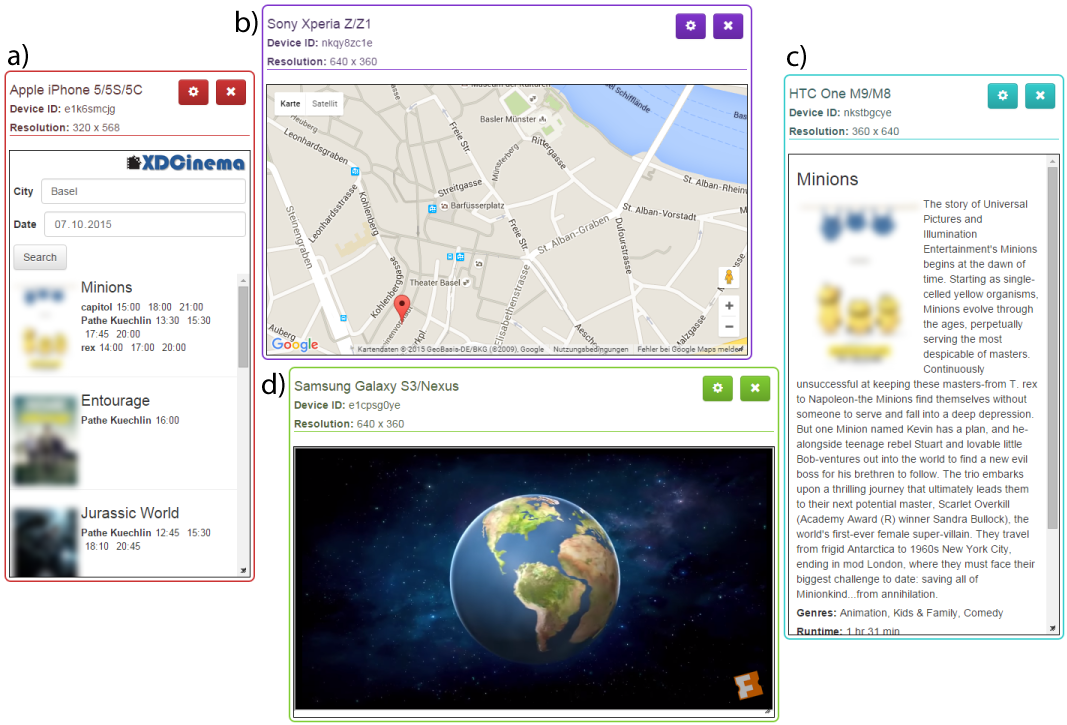
\includegraphics[width=1.0\textwidth]{images/screenshots/xdcinema_5_labeled.png}
	\caption[Screenshot XDCinema: Different views]{Different views of XDCinema}
	\label{fig:xdcinema}
\end{figure}

Depending on the number of devices that are connected, the four views are distributed differently. The trailer view is shown when the link to the trailer in the movie view is clicked and is only shown when at least four devices are connected. Otherwise, the link is just opened in a new tab on the device with the movie view. If only one device is connected, the remaining three views are all shown on that device and when the user navigates away from the search view they can get back to the search view using a back button. When two devices are connected, the movie view and the location view are both moved to the second device and the view that is shown depends on where the user last clicked in the search view. If the user clicks on a movie in the search view, the movie view is shown; if they click on a cinema, the location view is shown. If three devices are connected, the three views are distributed among all three devices. If more than four devices are connected, all additional devices do not show anything.

\subsection{Implementation}

XDCinema was implemented using the XD-MVC framework, but without Polymer. Thus, it is just a normal web application that accesses the JavaScript API of XD-MVC. Due to the difficulty of finding suitable APIs in the cinema and movie domain, the data that is used in the application is statically encoded in a JavaScript file. However, the application could easily be extended to support access to an API instead. The DOM on each device contains all four application views and all except the appropriate application view are hidden depending on the role of the device. 

Whenever a new device connects or a device disconnects, the roles are re-distributed and the views are updated. The available roles correspond to the four different application views, thus the role assignment is performed according to the rules of the view distribution described above. The role distribution happens randomly. The selected city, movie and cinema are shared between all connected devices through a shared variable that is synchronized using XD-MVC. When a shared variable is updated, each device performs the appropriate actions depending on its role. The selected city, movie, and cinema can only be changed from the search view. Therefore, all other devices only receive updates but do not send any updates themselves. If only one device is present, it has to hide the search view and location view if the selected movie is changed and it has to hide the search view and the movie view if the selected cinema changes. If the user wants to go back to the search view, it has to hide the location and movie view. If a device has both the movie and the location role, it has to hide the appropriate view when either the selected movie or the selected cinema changes. In cases where three or more devices are connected, the views that have to be hidden do not change and only the information in the view has to be updated if the respective shared variable changes. 

\section{XDYouTube}

XDYouTube is a cross-device YouTube application that allows multiple people to watch videos together on one large screen. The application allows users to search for videos on their devices and add them to a queue. The videos in the queue are played one after another on a large screen. The users can also look at the currently playing video and the queued videos or pause and play the current video from their devices. The application is split into two different views, the controller view and the player view. In the player view (see Figure~\ref{fig:xdyt_player}), the current video is played. 

\begin{figure}[H]
  \centering
    
\includegraphics[width=1.0\textwidth]{images/screenshots/xdyt/player_2.png}
	\caption[Screenshot XDYouTube: Player view]{Player view of XDYouTube}
	\label{fig:xdyt_player}
\end{figure}

The controller view consists of two different parts:
\begin{itemize}
	\item In the first part, the user can search for videos. If the user searches for a video, a list of results is displayed. For each result, the thumbnail, title and description of the video is displayed. The user can click on a button to add the video to the queue. They can also navigate to the next page of search results.
	\item In the second part, the user sees the title, thumbnail and description of the video that is currently played. They can also pause or continue the video. The user also sees the thumbnails and titles of the videos that are still in the queue. 
\end{itemize}

On large devices, both parts of the controller view are displayed simultaneously. On smaller devices, the first part is only shown in portrait mode (see Figure~\ref{fig:xdyt_controller_portrait}. The second part is only shown in landscape mode (see Figure~\ref{fig:xdyt_controller_landscape}).

\begin{figure}[H]
  \centering
    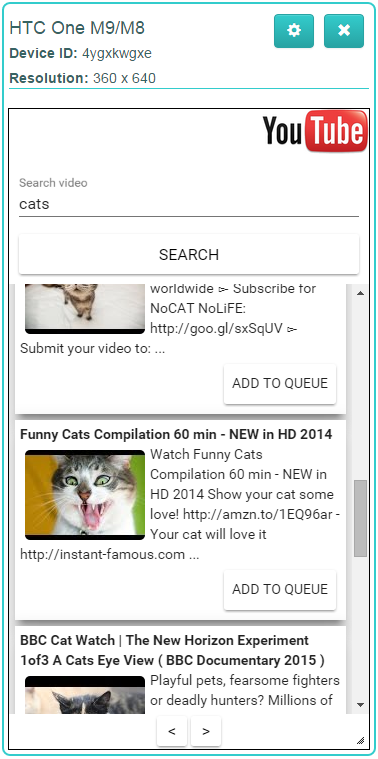
\includegraphics[width=0.6\textwidth]{images/screenshots/xdyt/controller_portrait_2.png}
	\caption[Screenshot XDYouTube: Controller view (first part)]{First part of the controller view in XDYouTube}
	\label{fig:xdyt_controller_portrait}
\end{figure}

\begin{figure}[H]
  \centering
    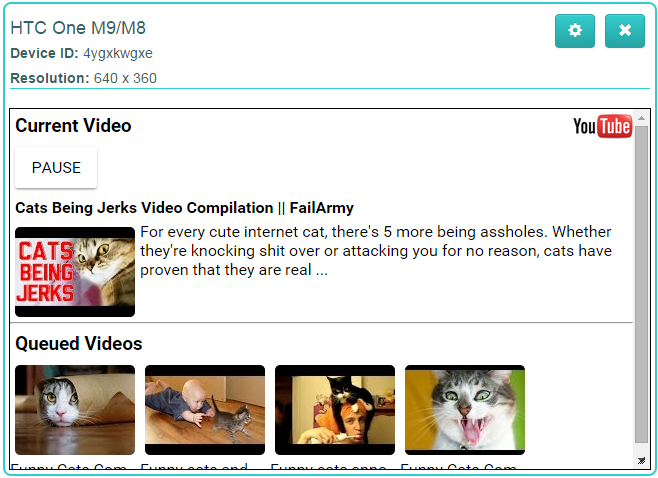
\includegraphics[width=0.9\textwidth]{images/screenshots/xdyt/controller_landscape_2.png}
	\caption[Screenshot XDYouTube: Controller view (second part)]{Second part of the controller view in XDYouTube}
	\label{fig:xdyt_controller_landscape}
\end{figure}

The device with the largest resolution automatically shows the player view. All other devices show the controller view. 

\subsection{Implementation}

XDYouTube is implemented with XD-MVC in combination with Polymer. The devices in the application can have three different roles:
\begin{itemize}
	\item "player": This role is assigned to the largest device.
	\item "controller": This role is assigned to all devices except the largest device.
	\item "xlarge": This role is assigned to devices with a width of more than 1000 pixels.
\end{itemize}
Depending on the role and the orientation of a device, different views are shown. As described above, the device with the role "player" shows the player view. Devices with the roles "xlarge" and "controller" show both parts of the controller view simultaneously, devices that only have the role "controller" show only one part of the controller view, depending on the orientation. Whenever a new device connects or a device disconnects, the roles and thus also the views are updated to reflect the new device configuration.

\section{Insights}

While developing the sample applications, we used XDTools. However, the implementation of XDTools was not complete yet at that point and some ideas emerged only from developing those applications. Before starting with the development of the sampling applications, the devices had to be connected manually. During the development, we realized that constantly re-connecting devices is one of the most time-consuming tasks while developing cross-device applications. From this, we came up with the idea of automatic connection management. Furthermore, we noticed that we often wanted to look at the JavaScript of the devices. But locating the correct file for a device was a difficult task, and the subdomains generated by our DNS server complicated things even more. Every device has its own subdomain and we first had to look for the subdomain of the device, then locate the subdomain in the large list of domains in the browser debugging tools, and finally navigating to the code that we want to look at. This made it evident that some mechanism for opening files or functions on a specific device was required. Thus, we integrated function debugging into XDTools. 

Developing the sample applications also helped with locating and fixing some bugs. It also gave us some ideas for further improvements that are not yet included with XDTools. One example is the positioning of emulated devices: Right now, devices are always added in the top left corner of the device emulation space. Therefore, the developer always has to move the devices away from this location because otherwise the devices would overlap. Some algorithm that automatically looks for a free space where the emulated device can be added would help solve this problem and make creating devices even more efficient.

In general, XDTools already helped a lot while developing the sample applications. Adding multiple emulated devices that do not share any local resources was probably the most useful feature of XDTools. However, the shared JavaScript console also proved helpful while developing the sample applications. We did not use record and replay very often during the development of the applications. In hindsight, we can think of a few situations where it might have been useful, but in that situation, we did not think about using record and replay. Record and replay is a feature that has not often been used previously by developers, and we did not use it before either, thus it might take some time to get used to it and recognize situations where it is useful. Furthermore, our sample applications are rather simple and did not require extensive debugging. However, as far as we can tell from our development experience, XDTools already helps a lot when developing a cross-device application.
\chapter{Evaluation}

After implementing our tools, we conducted a user study with our tools. The goal of the study was to evaluate the suitability and quality of our tools. Thus, we designed multiple tasks that the participants had to complete with our tools. Because we need something to compare our results to, the participants also completed some tasks without our tools, using only the browser tools available in Google Chrome. In the following sections, we will describe the setup of the study, present our results and conclude with a discussion of our results.

\section{Setup}

The study was carried out in a room of the GlobIS group. The participants were sitting in front of a desktop PC with a 30-inch screen with a 2560x1600 resolution and had access to an English (US) keyboard and a mouse. The desktop PC was running Microsoft Windows 7 with Google Chrome Version 45. They also had access to two real devices: An Asus Nexus 7 (2012 version) Android tablet and an HTC M9 Android phone. Furthermore, they were given a tutorial sheet about JavaScript that contained some functions that are useful for DOM modification as well as arrays. Figure~\ref{fig:study_setup} shows a picture of the setup of the study.

\begin{figure}[H]
  \centering
    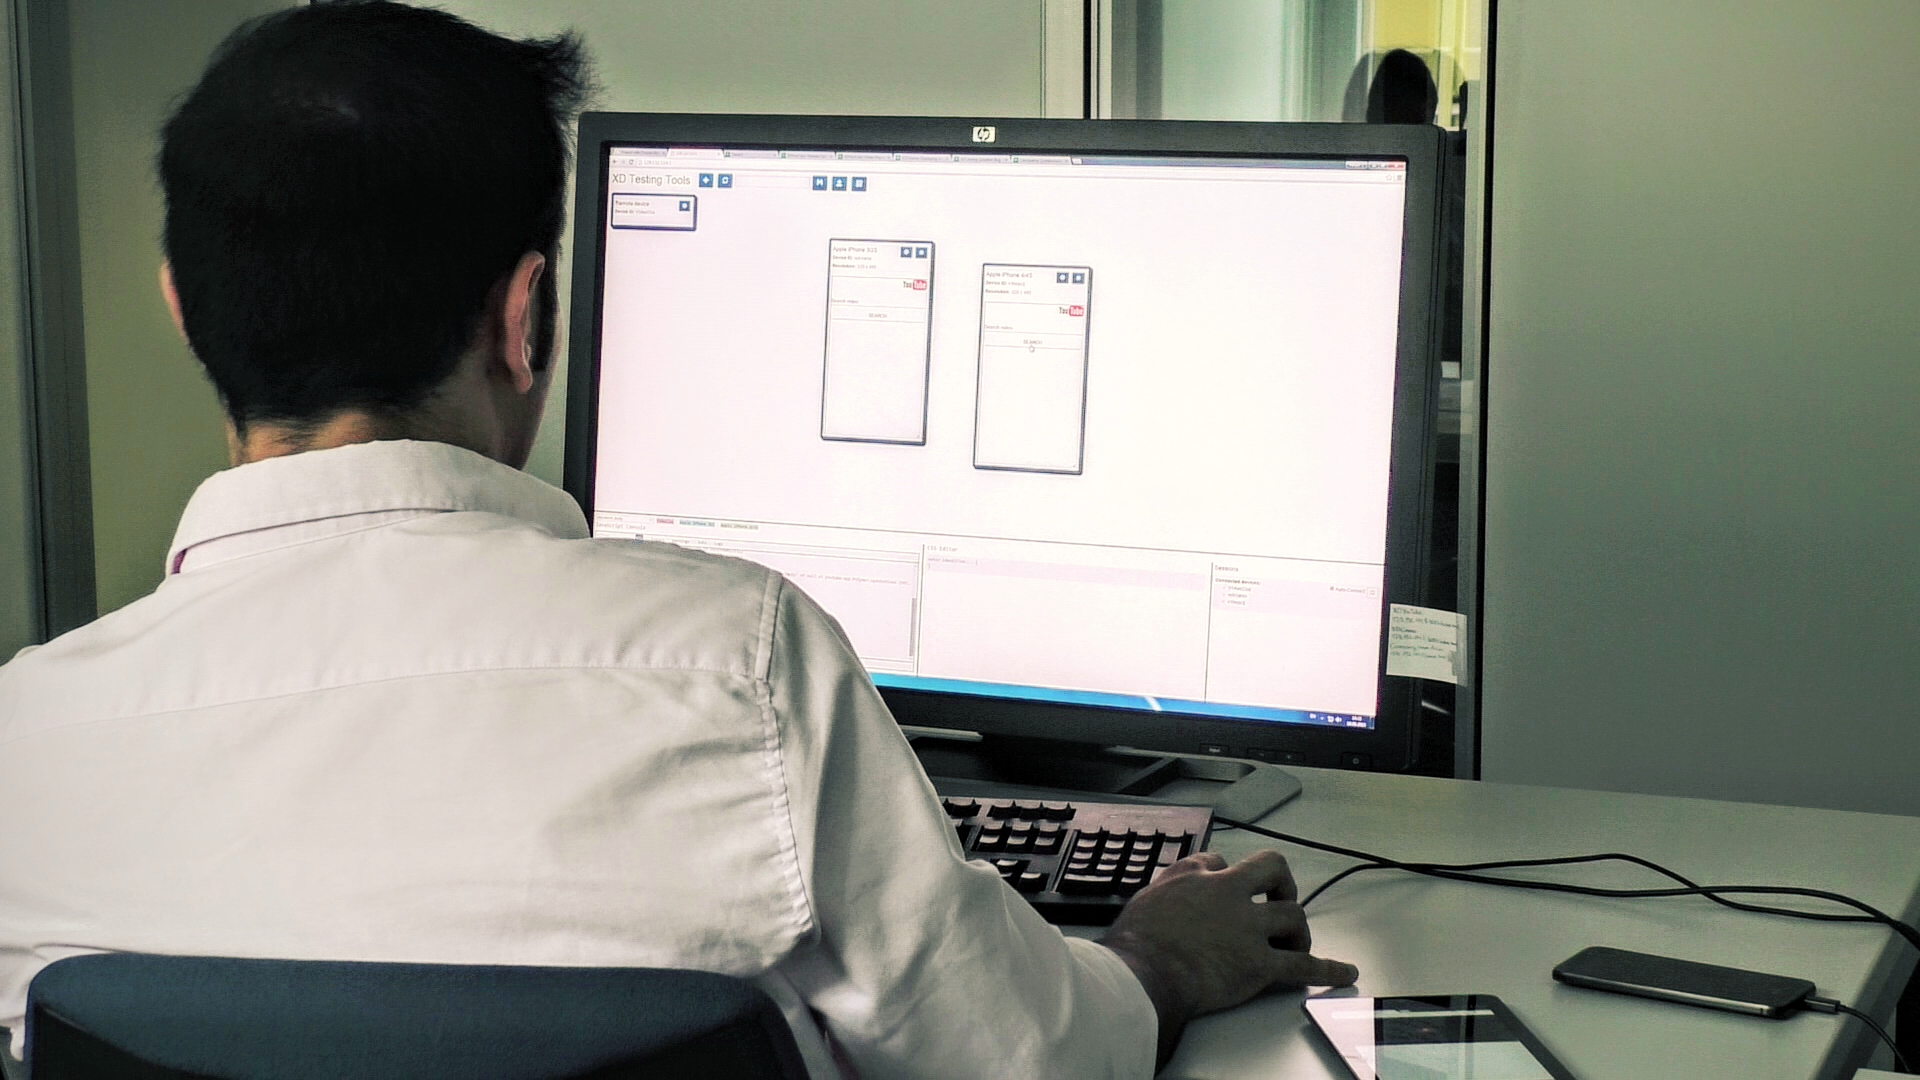
\includegraphics[width=0.8\textwidth]{images/study_setup2.png}
	\caption[Photo: Study setup]{Study Setup}
	\label{fig:study_setup}
\end{figure}

During the study, the instructor was sitting next to the participants and was available to answer any questions that occurred during the study. If a participant did not make any progress on a task for some time, the instructor also gave some hints to lead the participant in the right direction.

The participants had access to Chrome DevTools for all tasks. Furthermore, we set up multiple profiles on Chrome that the participants could use for emulating multiple devices. The participants could also remote debug the two real devices they had access to. The devices were already connected to the desktop PC by cable and the appropriate tab was already opened in the browser. Thus, the participants only had to navigate to the tab and click on inspect to remote debug a device. 

During the study, we disabled some features of our tools that were not required for completing the tasks so the participants would not be overwhelmed with the large amount of features that they had to learn how to use. We disabled the following features:
\begin{itemize}
	\item Changing the URL: The URL was given by the task anyway and it would have been of no use to change it during the study.
	\item Saving and loading device configurations: This feature is mainly useful for long-term use of our tools and is not needed for completing the tasks in the study.
	\item Record/Replay: We think that record/replay takes some time to get used to it and it is also only of limited use for simple tasks like the ones we used in the study. Furthermore, it might distract participants from the actual task because they might want to try it out even if it does not help them to complete the task.
	\item Inspecting HTML: The tasks in our study did not require modification or debugging of HTML, thus we deactivated this feature.
	\item Settings: The settings were disabled for the study because they were implicitly given by us.
\end{itemize}

All other features could be used by the participants. The following list provides an overview of the features the participants had access to:
\begin{itemize}
	\item Emulating devices
	\item Connecting real devices
	\item Connection features (auto-connect and drop-down list to connect to other devices)
	\item Shared JavaScript console
	\item Function debugging
	\item Shared CSS Editor
\end{itemize}
This list also represents the features that we want to evaluate during the study.

\subsection{Participants}

We recruited 12 participants that all were university members in the department of computer science at ETH Zurich. Most participants were either PhD or Master students, but there were also some Bachelor students. It was required that all participants have at least basic knowledge about front-end web technologies (i.e. HTML, CSS, JavaScript). However, the definition of "basic" was up to the participants and we did not ask participants to prove their experience before the study. Consequently, we also had some participants that had rather low experience with web technologies. We did not require participants to have any experience with cross-device application development as otherwise it would have been difficult to find enough participants. Nevertheless, two thirds of the participants actually did have some cross-device application development experience. The age of the participants ranged from 23 to 33 and the median age was 26. 

\subsubsection{Previous Experience}
We asked all participants about their previous experience with web application development and JavaScript in particular, as well as about their previous experience with responsive web applications and cross-device web applications. Furthermore, we asked them about whether they have used Chrome DevTools before and how they used them. The participants rated their skills in web application development and JavaScript on a 5-point Likert scale (see Figure~\ref{fig:xp}) from basic to proficient and also gave the numbers of years in experience (see Figure~\ref{fig:years_of_xp}) that they had in web application development and JavaScript.

\begin{figure}[H]
  \centering
    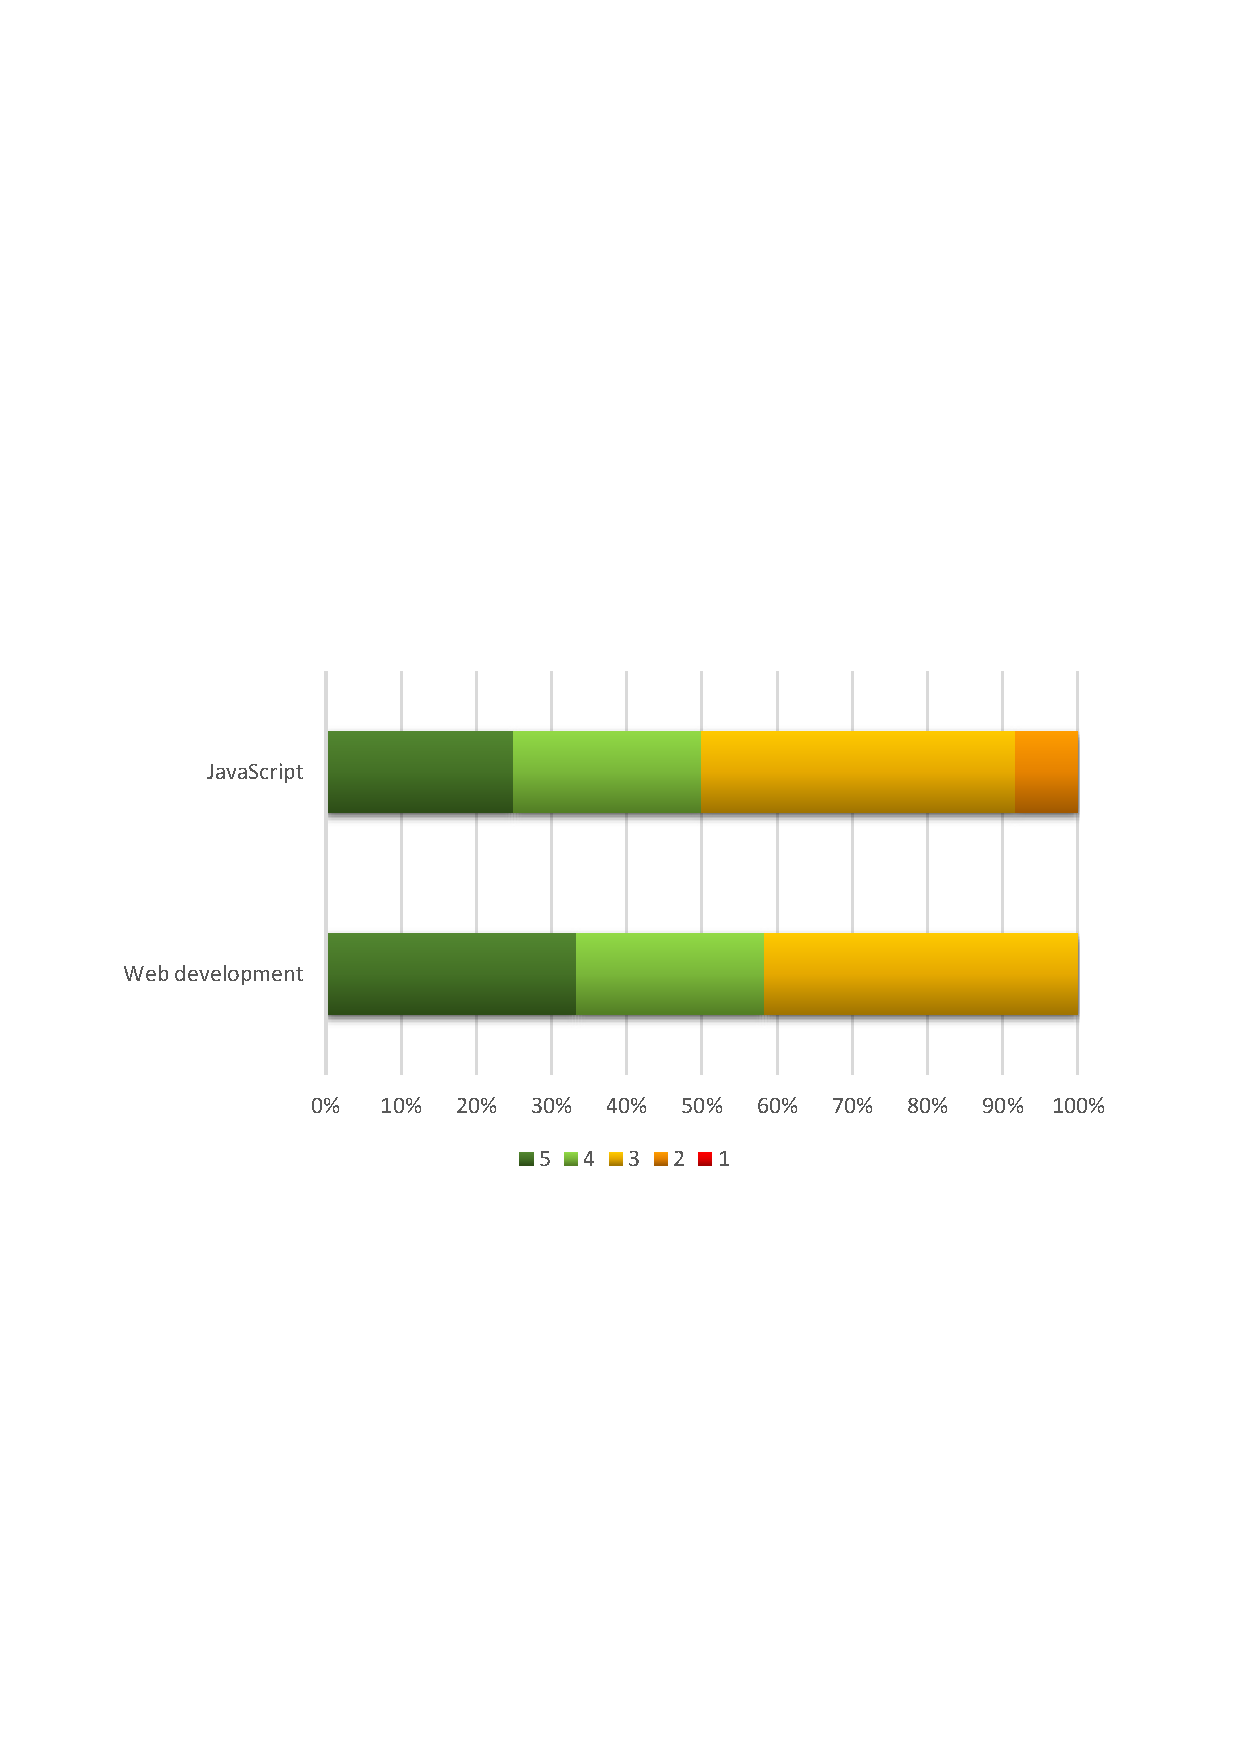
\includegraphics[width=0.8\textwidth]{images/charts/xp.pdf}
	\caption[Previous experience of participants]{Previous experience}
	\label{fig:xp}
\end{figure}

\begin{figure}[H]
  \centering
    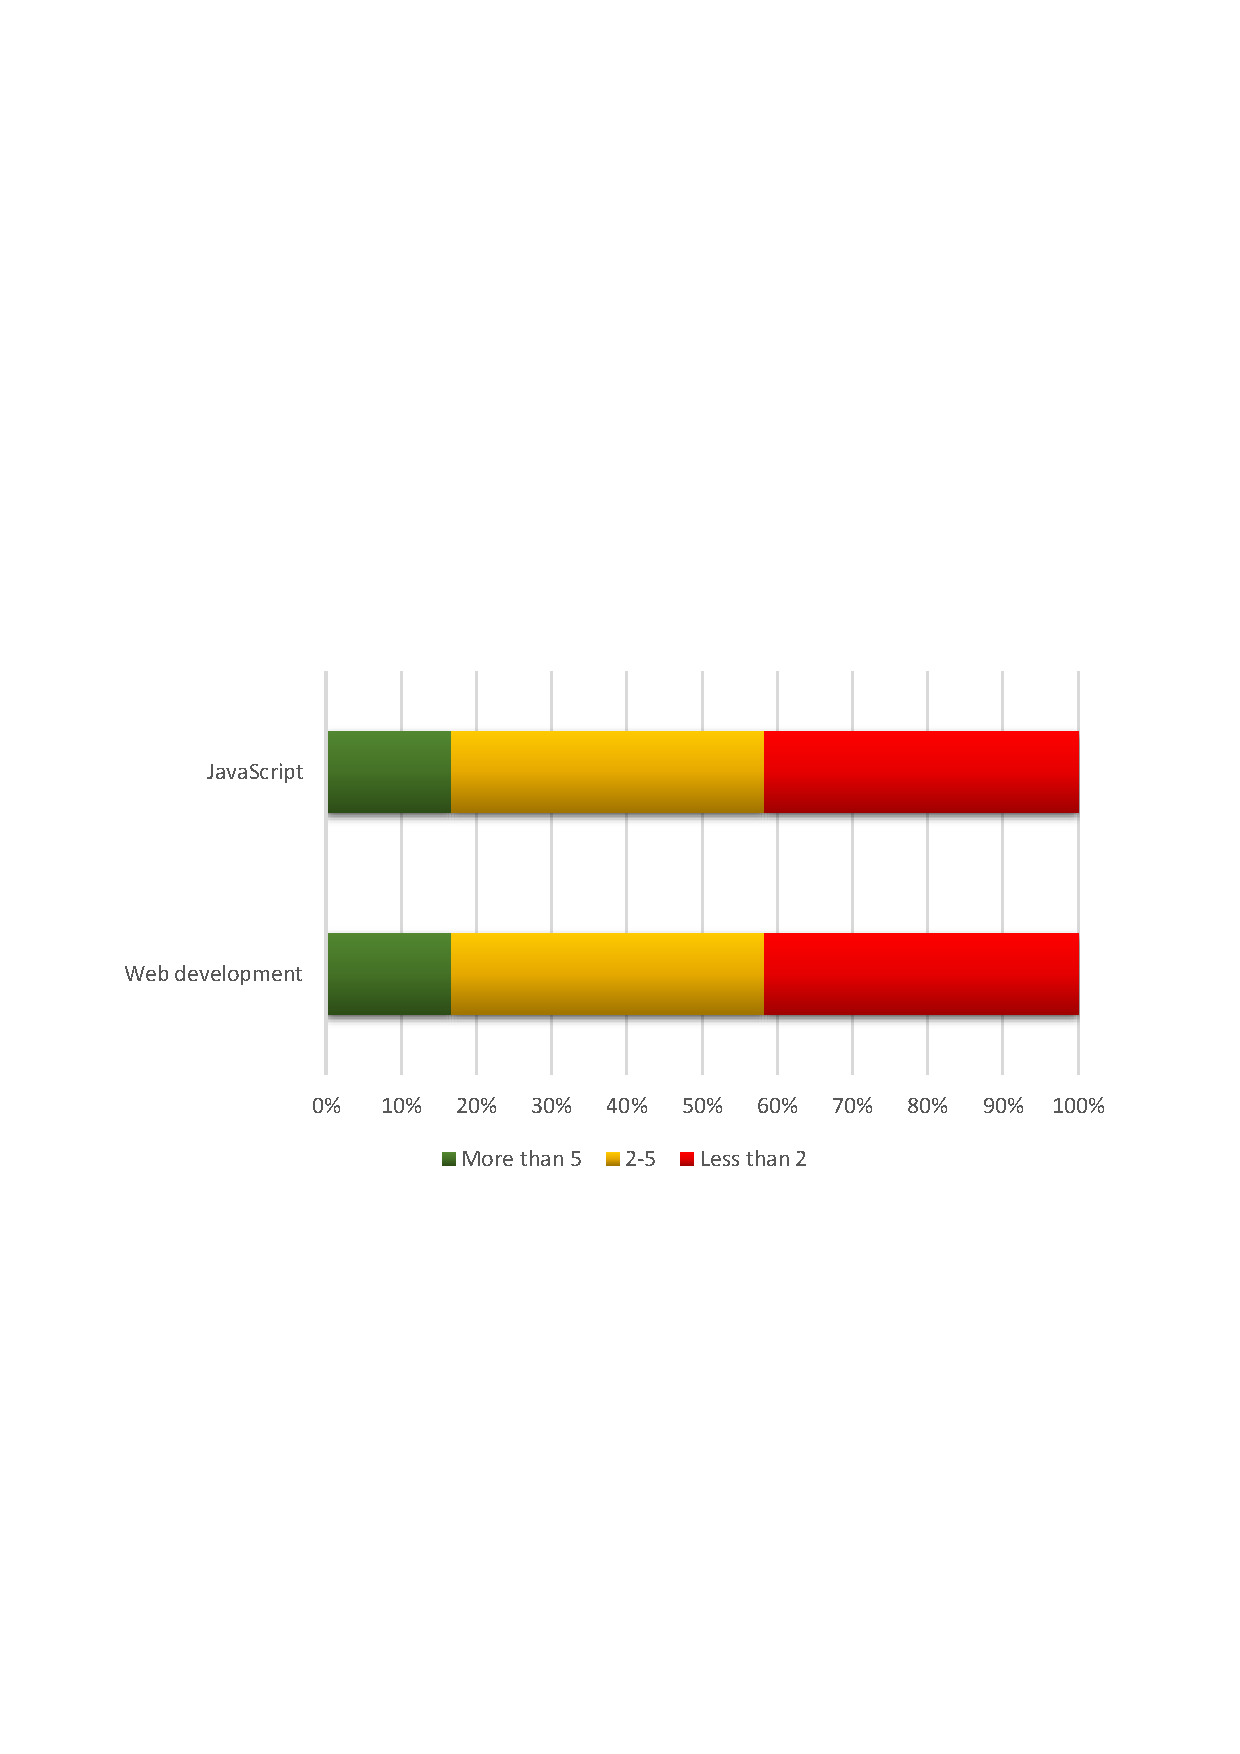
\includegraphics[width=0.8\textwidth]{images/charts/years_of_xp.pdf}
	\caption[Years of experience]{Years of experience}
	\label{fig:years_of_xp}
\end{figure}

Nine out of the twelve participants stated that they already had some experience with developing responsive web applications. All except one used browser tools for emulating devices for testing their applications and all except two used real devices. Only one participant stated that they only used real devices for testing and no browser tools. One participant mentioned that they mainly re-sized browser windows to test their applications.

Eight participants already had some experience with cross-device application development. Again, most of them used browser tools for emulating devices and/or real devices for testing their applications. Four of them either used multiple browsers, multiple browser profiles or incognito modes to emulate multiple devices on one device. The fact that the other participants did not use any of those tools indicates that they probably used multiple devices at all times. This could either be because they do not know that they exist, because they are inconvenient or because they simply prefer real devices.

Most of the participants already had experience with Chrome DevTools, only two participants indicated that they had never used them before and one of them had used the developer tools of Firefox instead. We asked participants how often they used certain features of Chrome DevTools, in particular Device Mode, HTML and CSS inspection, JavaScript debugging and the console (see Figure~\ref{fig:devtools_xp}). Not all participants had used Device Mode, which is no surprise, given that it is a rather new feature. All participants stated that they often use HTML and CSS inspection, thus this seems to be the most popular feature. The console was also used rather often. Surprisingly, JavaScript debugging was not that popular, less than half of the participants stated that they often use it.

\begin{figure}[H]
  \centering
    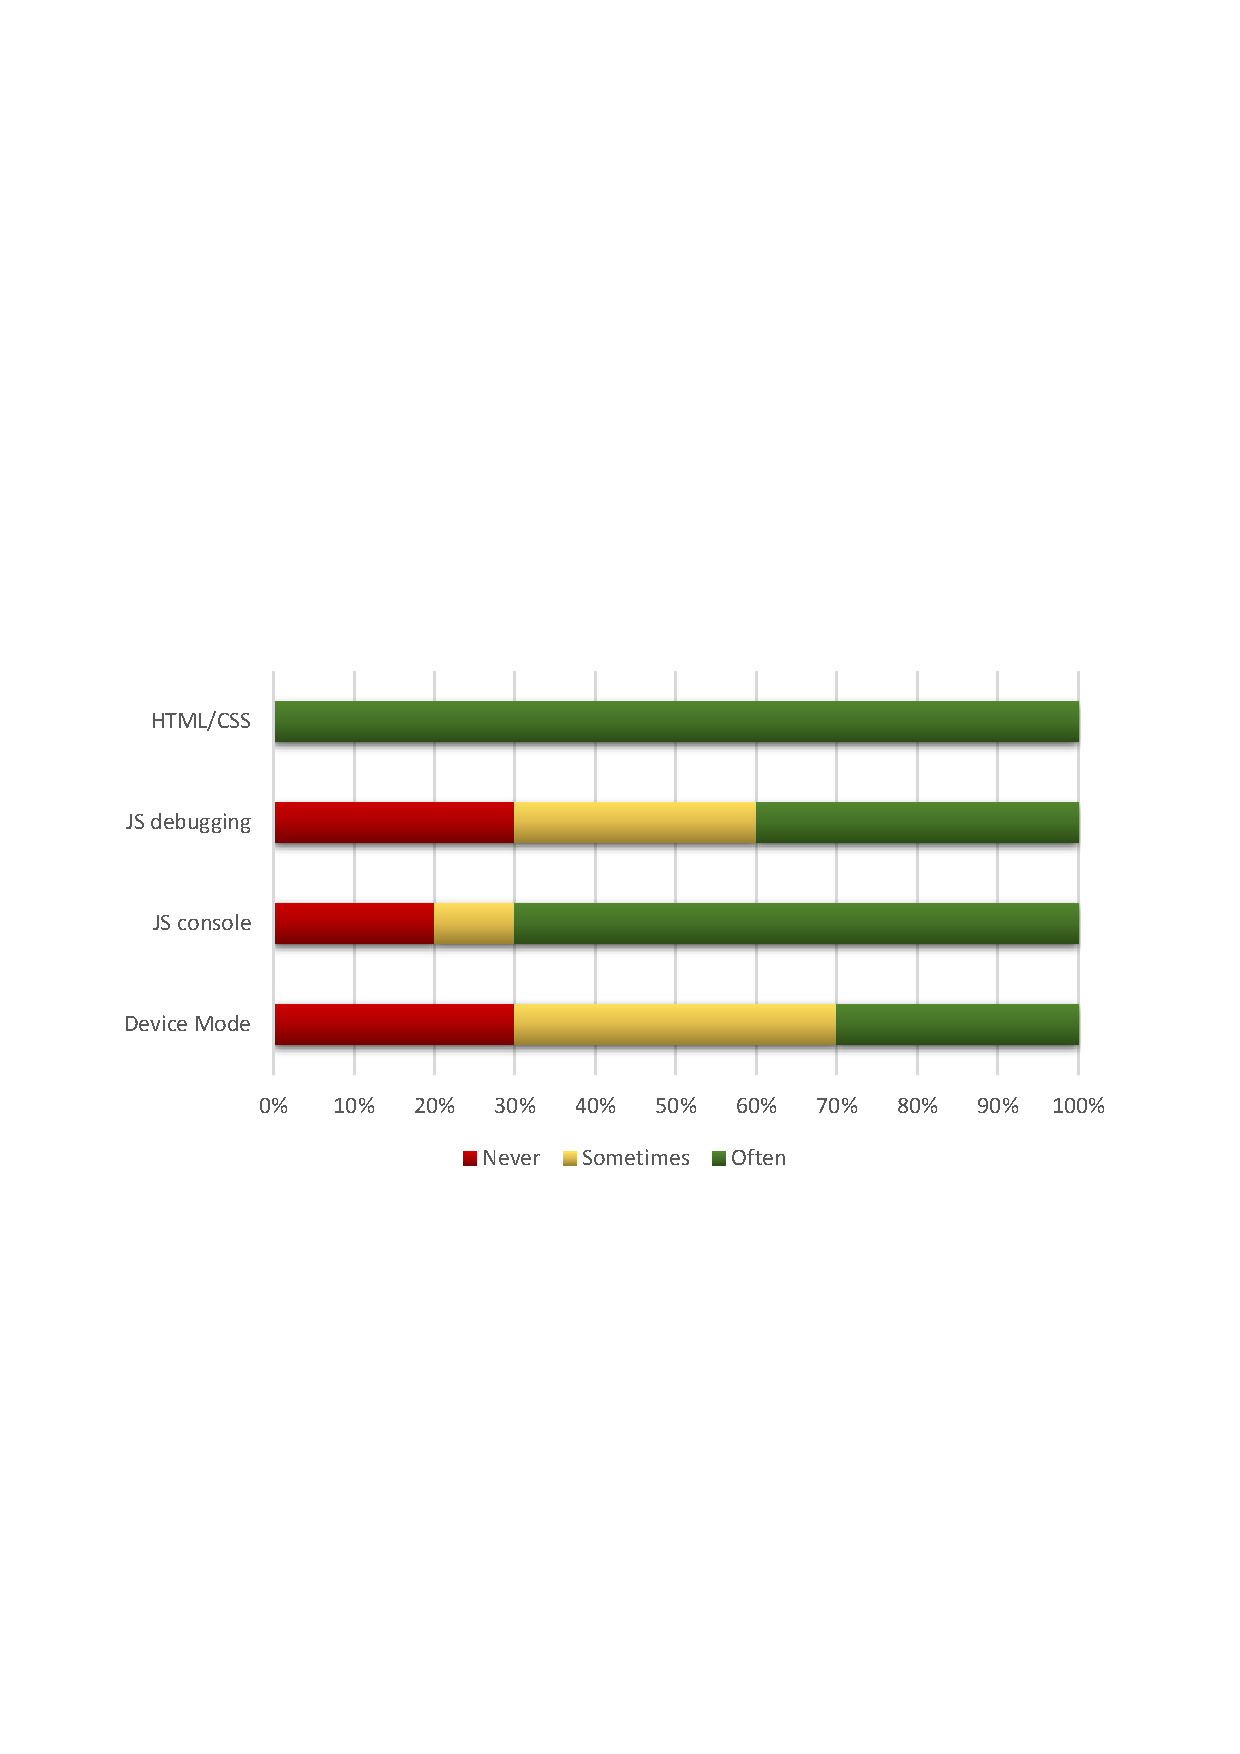
\includegraphics[width=0.8\textwidth]{images/charts/devtools_xp.pdf}
	\caption[Previous experience with Chrome DevTools]{Previous experience with Chrome DevTools}
	\label{fig:devtools_xp}
\end{figure}

\subsection{Tasks}

We used two different applications for the tasks, namely the two sample applications that we described earlier, XDCinema and XDYouTube. For each application, there were two tasks; one was about finding and fixing a bug in the code, and the other one was about implementing a new feature. The maximum time for the tasks where the participants fixed a bug was 15 minutes and the maximum time for implementing a feature was 30 minutes. After this time, we aborted the task unless it was clear that the participants would finish within the next 2 to 3 minutes. Each participant had to complete all four of the tasks; the tasks of one application with our tools, the tasks of the other application without them. The order of the applications as well as whether the first two tasks were with or without the tools was random. The participants completed the debugging task first and then the implementation task. Thus, the participants could learn how to use the application during the debugging task, which was considered easier than the implementation task, and were already familiar with the application for the second task.

\subsubsection{XDYouTube}
XDYouTube allows users to use their personal devices to search for videos and add them to a queue. The videos from the queue are then played one after the other on the largest of the devices. Users can also see the title and description of the currently playing video as well as the videos that are still in the queue by switching their device into landscape mode.

The first task (xdyt-bug) with XDYouTube was to fix a bug concerning the video queue. As soon as one video finishes playing, the next video is dequeued from the queue and starts playing. However, when no video is in the queue, a JavaScript error occurs and causes the next video that is added to the queue not to play. The users were given a description of the task and then had to reproduce and fix it.  The participants were given a JavaScript file with two functions, one that adds a video to the queue and one that loads the next video at the end of a video.

For the second task (xdyt-impl), we asked participants to implement a remote control that can play and pause the current video from the controller devices. The participants had to implement two functions: One was called when the remote control button was clicked (the button as well as the event handler were already implemented), the other was called when a shared variable that states whether the video is paused or playing is changed. Thus, the participants had to change the shared variable whenever the button was clicked and to react accordingly on all devices if the shared variable changes, i.e. they had to pause or play the video on the device that plays the video and they had to change the text of the remote control button from "Pause" to "Play" and vice versa on all other devices. Furthermore, they had to change the CSS of the button such that it looked similar to a picture of a button that was given to them. The participants were given a JavaScript file with the two empty functions as well as a CSS file with the empty CSS selector of the button. Furthermore, they had access to a few helper functions:
\begin{itemize}
	\item pauseVideo(): Pauses the video
	\item unpauseVideo(): Unpauses the video
	\item isVideoPlaying(): Returns true if any video is currently active (even if it is paused)
	\item setPausedState(state): Sets the state of the shared variable
	\item getPausedState(): Returns the state of the shared variable (true if paused, false if playing)
	\item isPlayer(): Returns true if the device is responsible for playing the video and false if not
	\item isController(): Returns true if the device is responsible for controlling the video (add videos to queue, etc.) and false otherwise
\end{itemize}

\subsubsection{XDCinema}

XDCinema allows users to search for a city and date on one device. The device then shows a list of movies that play in this city on that date as well as the cinemas where the movie is played and the time that the movie starts. If the user clicks on a cinema, a summary of the movie as well as other information about the movie is shown on another device. If the user clicks on a cinema, the location of the cinema is shown on another device.

The first task (xdc-bug) was to fix a bug where the location of most cinemas was displayed wrongly, even though the information in the database is correct. The bug was that in one function, "j" was used instead of "i", which caused a wrong location to be returned. The participants were given a JavaScript file with a few functions related to getting and updating the location on all devices.

In the second task (xdc-impl), the participants first had to complete the implementation of a function that shows the prices of each cinema where the movie plays below the description of the cinema. A skeleton for this function was already given where a loop over all cinemas that show the movie was already implemented, the participants only had to fill in the body of the loop. The second part of the task was to highlight the correct price (the participants were given a CSS class called "highlighted") when the user clicks on a cinema in the search view and to improve the CSS for highlighting. In the original version, highlighting used a light grey background color and a white text color which was not very readable. The participants were given a JavaScript file with the two functions as well as CSS file with the initial CSS of the "highlighted" class. The participants had access to the following helper function:
\begin{itemize}
	\item getCinemaPrice(cinemaName, city): Returns the price range of a cinema in a city
\end{itemize}

\subsection{Evaluation Methods}

In total, we used four different methods for evaluating the results of our user study. During the study, the participants had to fill out multiple questionnaires. Most our results are based on the questionnaires, the other methods for evaluation are only for clearing any inconsistencies, finding explanations for some things and maybe gathering some additional information that we missed during the study.

\subsubsection{Questionnaires}
At the beginning of the study, each participant had to fill out a questionnaire about their background information. The results of this questionnaire were already presented earlier. After each task, the participant had to fill out another questionnaire with the following questions:
\begin{itemize}
	\item It was easy to complete the task with the tools I had access to.
	\item I felt efficient completing the task with the tools I had access to.
	\item It was challenging to complete the task with the tools I had access to.
	\item The tools I had access to were well suited for completing the task.
\end{itemize}
The questions could be answered on a 5-level Likert scale from "Strongly Disagree" to "Strongly Agree". In the tasks where the participants had access to our tools, we also asked them to rate the usefulness of the individual features of our tools on a 5-level Likert scale. The following question was asked about the features: "How useful did you find the following features for completing the task?". The participants could answer this question for each feature on a 5-level Likert scale from "Not useful" to "Very useful". They could also choose the option "Not used" for features that they did not use while completing the task. For each task, there also was a comment field where the user could write down any additional comments that they had about the task or the tools they had access to.

After completing all tasks, the participants had to fill out a final questionnaire where they could answer some questions that compare our tools to the usual Chrome browser tools. They had to answer the following questions:
\begin{itemize}
	\item Did you find it easier to debug with or without the tool?
	\item Did you feel more efficient debugging with or without the tool?
	\item Did you prefer debugging with or without the tool?
	\item Did you find it easier to implement a feature with or without the tool?
	\item Did you feel more efficient implementing a feature with or without the tool?
	\item Did you prefer implementing a feature with or without the tool?
\end{itemize}
For those questions, the participants could either say that they preferred our tool, the normal browser tools, or that they did not have a preference.

In addition, they also answered some general questions about our tool.
\begin{itemize}
	\item It was easy to learn how to use the tool.
	\item I felt confident using the tool.
	\item The tool was unnecessarily complex.
	\item The tool would be useful for debugging cross-device applications.
	\item The tool would be useful for implementing cross-device applications.
	\item I would use the tool for debugging cross-device applications.
	\item I would use the tool for implementing cross-device applications.
\end{itemize}
Those questions could again be answered on a 5-level Likert scale from "Strongly Disagree" to "Strongly Agree".

Finally, the participants could state which features of the tool they would use for debugging and implementing cross-device applications and they could also write some comments about the tool if they wanted to.

\subsubsection{Video Recording}
In addition to letting participants fill out questionnaires, we also used a video camera to record the participants while completing the tasks. This was mainly done to make sure that no important information was lost and so some strategies for solving tasks could be extracted from the videos. 

\subsubsection{Personal Feedback}
At the end of the study, participants were encouraged to share any comments that they still wanted to mention and to give their opinion about the tool. Any comments that the participants had given during the study were also noted.

\subsubsection{Time Measuring}
For each participant, the time required for completing each task was measured. This was mainly done to detect any major discrepancies between completion times with and without the tool. However, exact times are not considered relevant for evaluation because they highly depend on the participant and on the hints given by the instructor during the study.

\section{Results}

In the following sections, we will first present the results from the individual tasks and then the more general results. For each task, we will compare how people answered the questions in the per-task questionnaires with and without our tools. 

\subsection{XDCinema: Fixing a Bug}

The results for the task where the participants had to fix a bug in XDCinema can be seen in Figure~\ref{fig:xdc_bug_comparison}. The figure shows the median values for the questions asked after the task with and without our tools. For the question that asks about how challenging it was to complete the task with the tools the participant had access to, a lower value is better; for all other questions, a higher value is considered better. There is a rather big difference in the median value for the suitability of the tools, while the differences are smaller for the other questions. The participants felt only slightly more efficient when completing the task with our tools and considered the task as slightly less challenging. In the question about the easiness of the task, exactly the same median value can be observed both with and without our tools. One reason for the bigger difference in the suitability could be that unlike easiness and efficiency, suitability does not really depend on the task itself. In other words, if a task is difficult, the easiness will be rated lower regardless of whether our tools are used or not and if a task is time-consuming, the efficiency will be rated lower. On the other hand, the suitability of the tools for the task does not change with the difficulty or duration of the task. However, it would still be desirable that our tools make debugging cross-device applications easier and more efficient instead of just being more suited. For this task, it seems that our tools mainly made the task more enjoyable, but did not have any other effects. This could also be due to the fact that the bug is rather trivial and debugging does not necessarily help much anyway.

\begin{figure}[H]
  \centering
    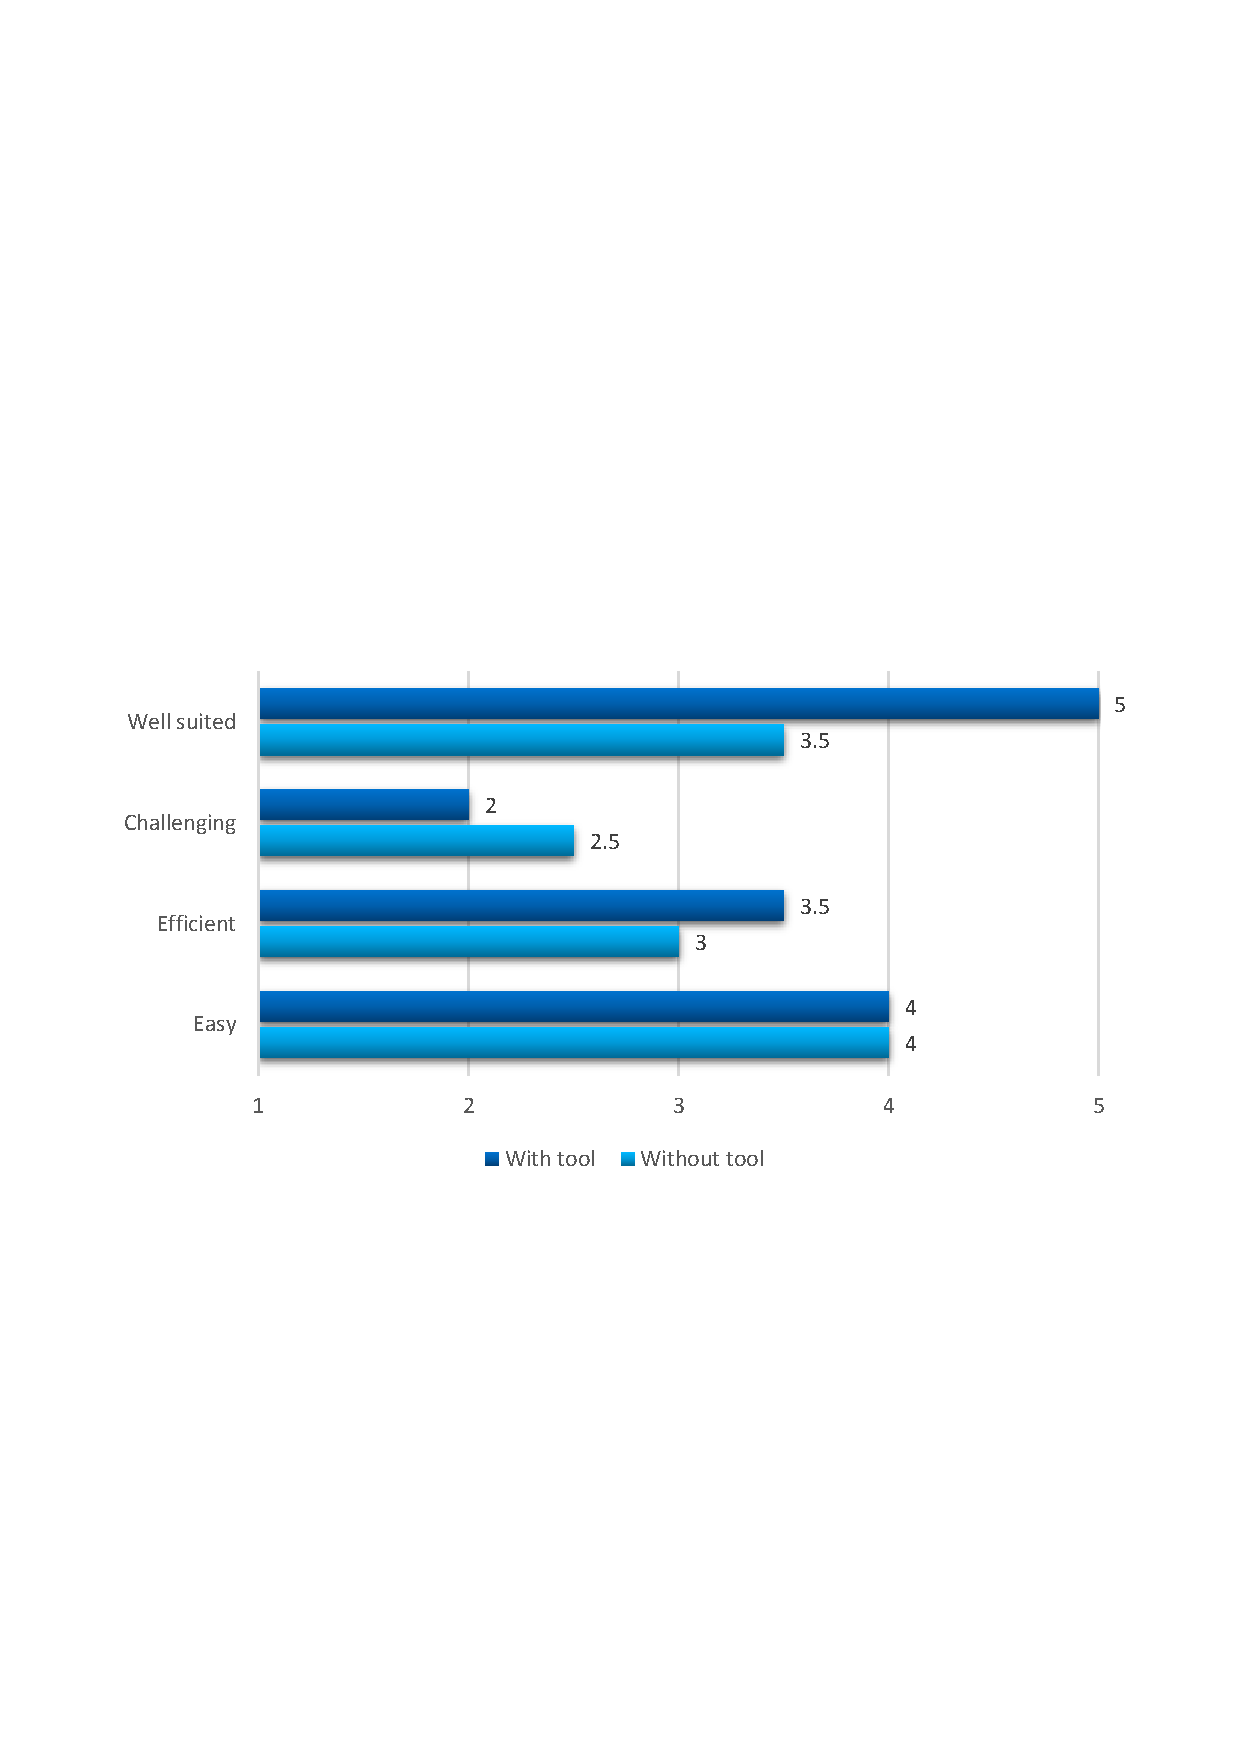
\includegraphics[width=0.8\textwidth]{images/charts/xdc_bug_comparison.pdf}
	\caption[xdc-bug: Comparison]{XDCinema debugging task - Comparison}
	\label{fig:xdc_bug_comparison}
\end{figure}

Figure~\ref{fig:xdc_bug_features_used} shows how many participants used the individual features of our tools and how useful they found them. Obviously, the figure only includes the participants that had access to our tools. None of the participants used real devices and all of them used device emulation instead. However, two participants rated device emulation with a 3, which indicates that they found it somewhat useful for the task, but not extremely useful. This could again be due to the fact that the bug they had to fix is actually rather trivial and could maybe even be solved faster by just looking at the code. The connection features and function debugging were used by all except one participant and were very appreciated by the participants. The shared JavaScript console was rather unpopular for this task, probably also due to the simplicity of the task and due to the fact that the bug produced no JavaScript errors that would be displayed in the console.

\begin{figure}[H]
  \centering
    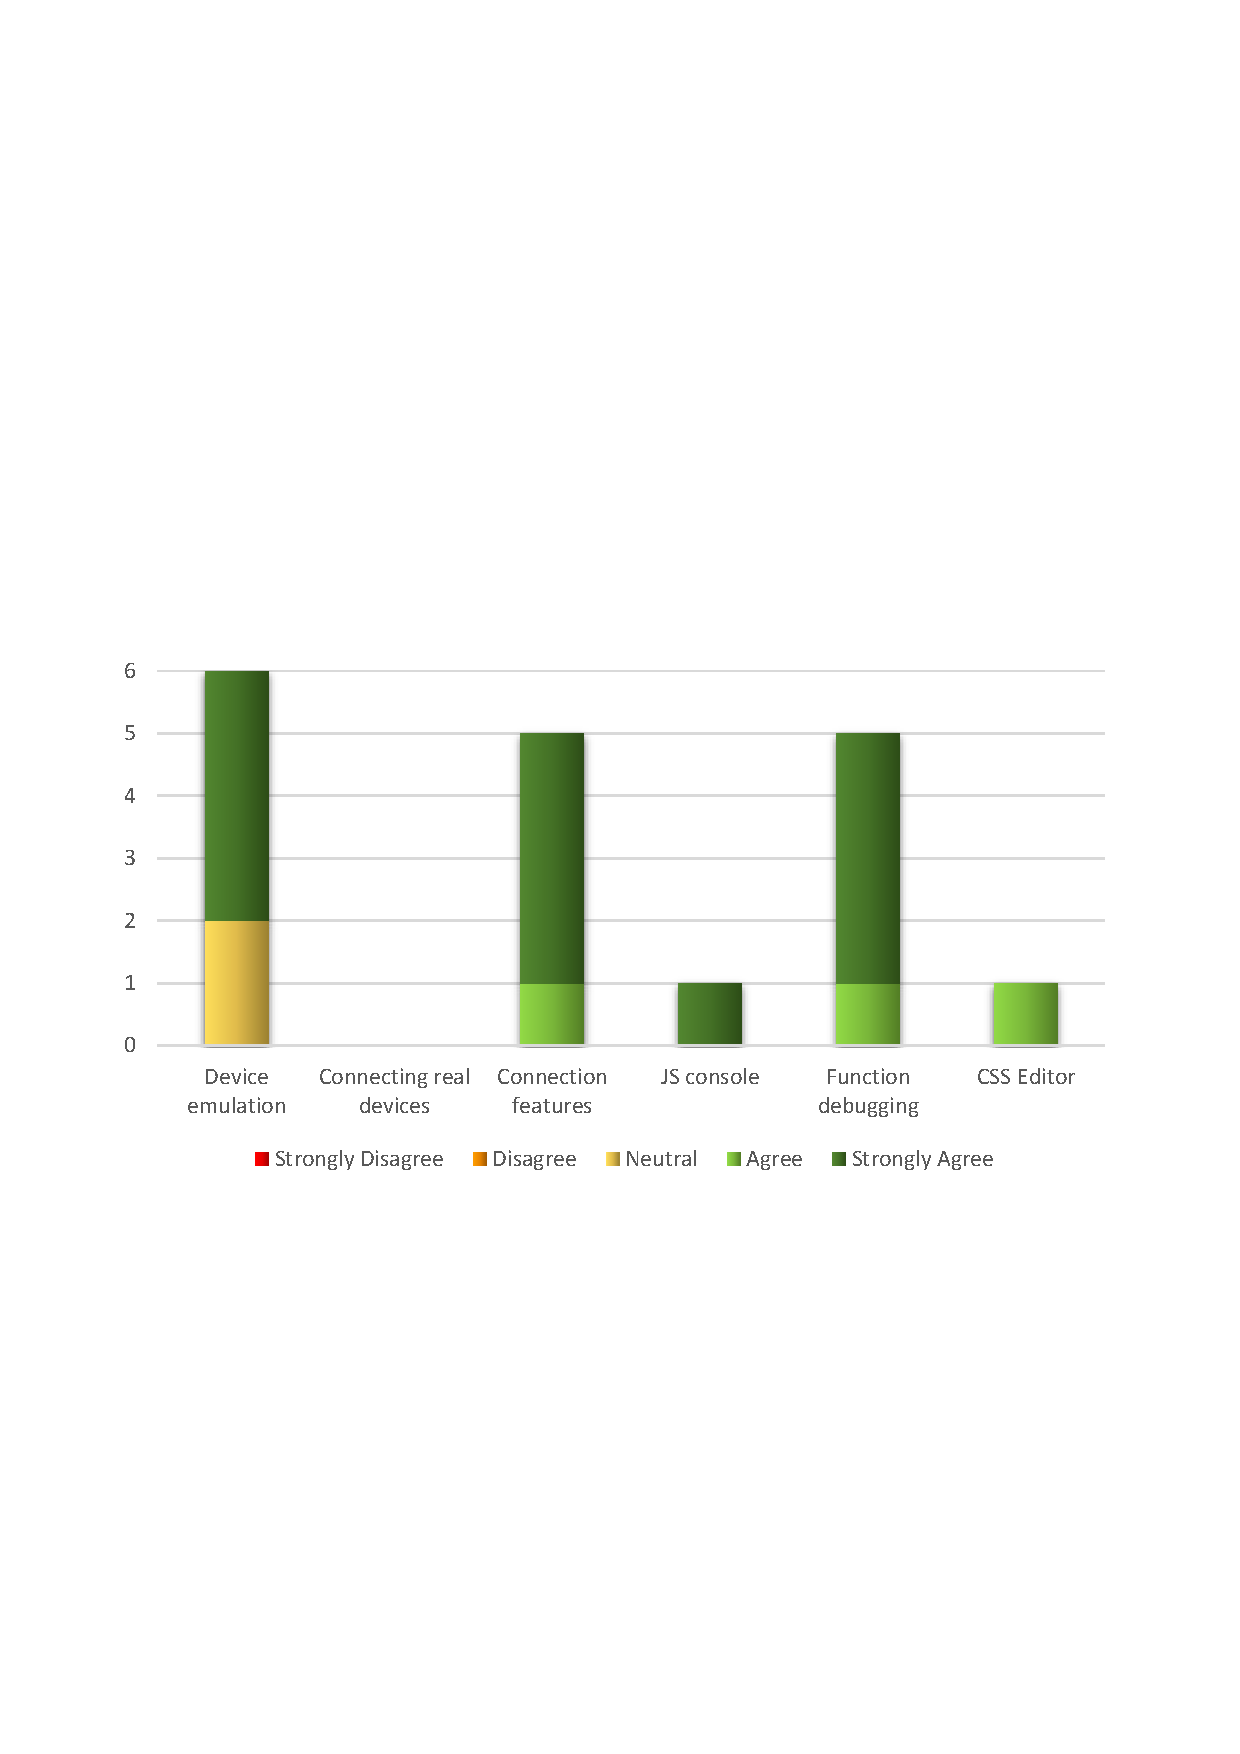
\includegraphics[width=0.8\textwidth]{images/charts/xdc_bug_features_used.pdf}
	\caption[xdc-bug: Features used]{XDCinema debugging task - Features used}
	\label{fig:xdc_bug_features_used}
\end{figure}

\subsection{XDCinema: Implementing a Feature}

In Figure~\ref{fig:xdc_impl_comparison}, the results for the implementation task in XDCinema can be seen. Again, the figure shows the median values. In this task, the difference in suitability is less pronounced than in the XDCinema debugging task, but the difference for the question about efficiency and easiness is larger. In general, the task was considered as rather easy independent of the tools the participant had access to, although participants that had access to the tools perceived it as even easier. The median value of five with our tools suggests that participants had no problems completing the task at all when they had access to our tools. Similar results can be observed concerning efficiency. The difference in median values suggests that the participants felt quite a bit more efficient with our tools. Surprisingly, if we compare the average and median completion times for this task, the participants that had access to our tools were considerably slower (comparing median values, the participants that had access to our tools were about 9 minutes slower). In fact, this is the only task where the difference in completion times with and without our tools is noticeable; the completion times for all other tasks are almost equivalent. However, those two facts do not necessarily contradict each other, as there were participants with very different experience levels and as it is random which participants have access to our tools and which not and the number of participants is rather low, it is possible that almost all participants with low experience fall into the same category. In general, the completion times should not be considered as especially relevant, after all the instructor also gave some hints during the study and this can also distort completion times significantly. However, it would be interesting to see how completion times differ if there is a larger number of participants. 

\begin{figure}[H]
  \centering
    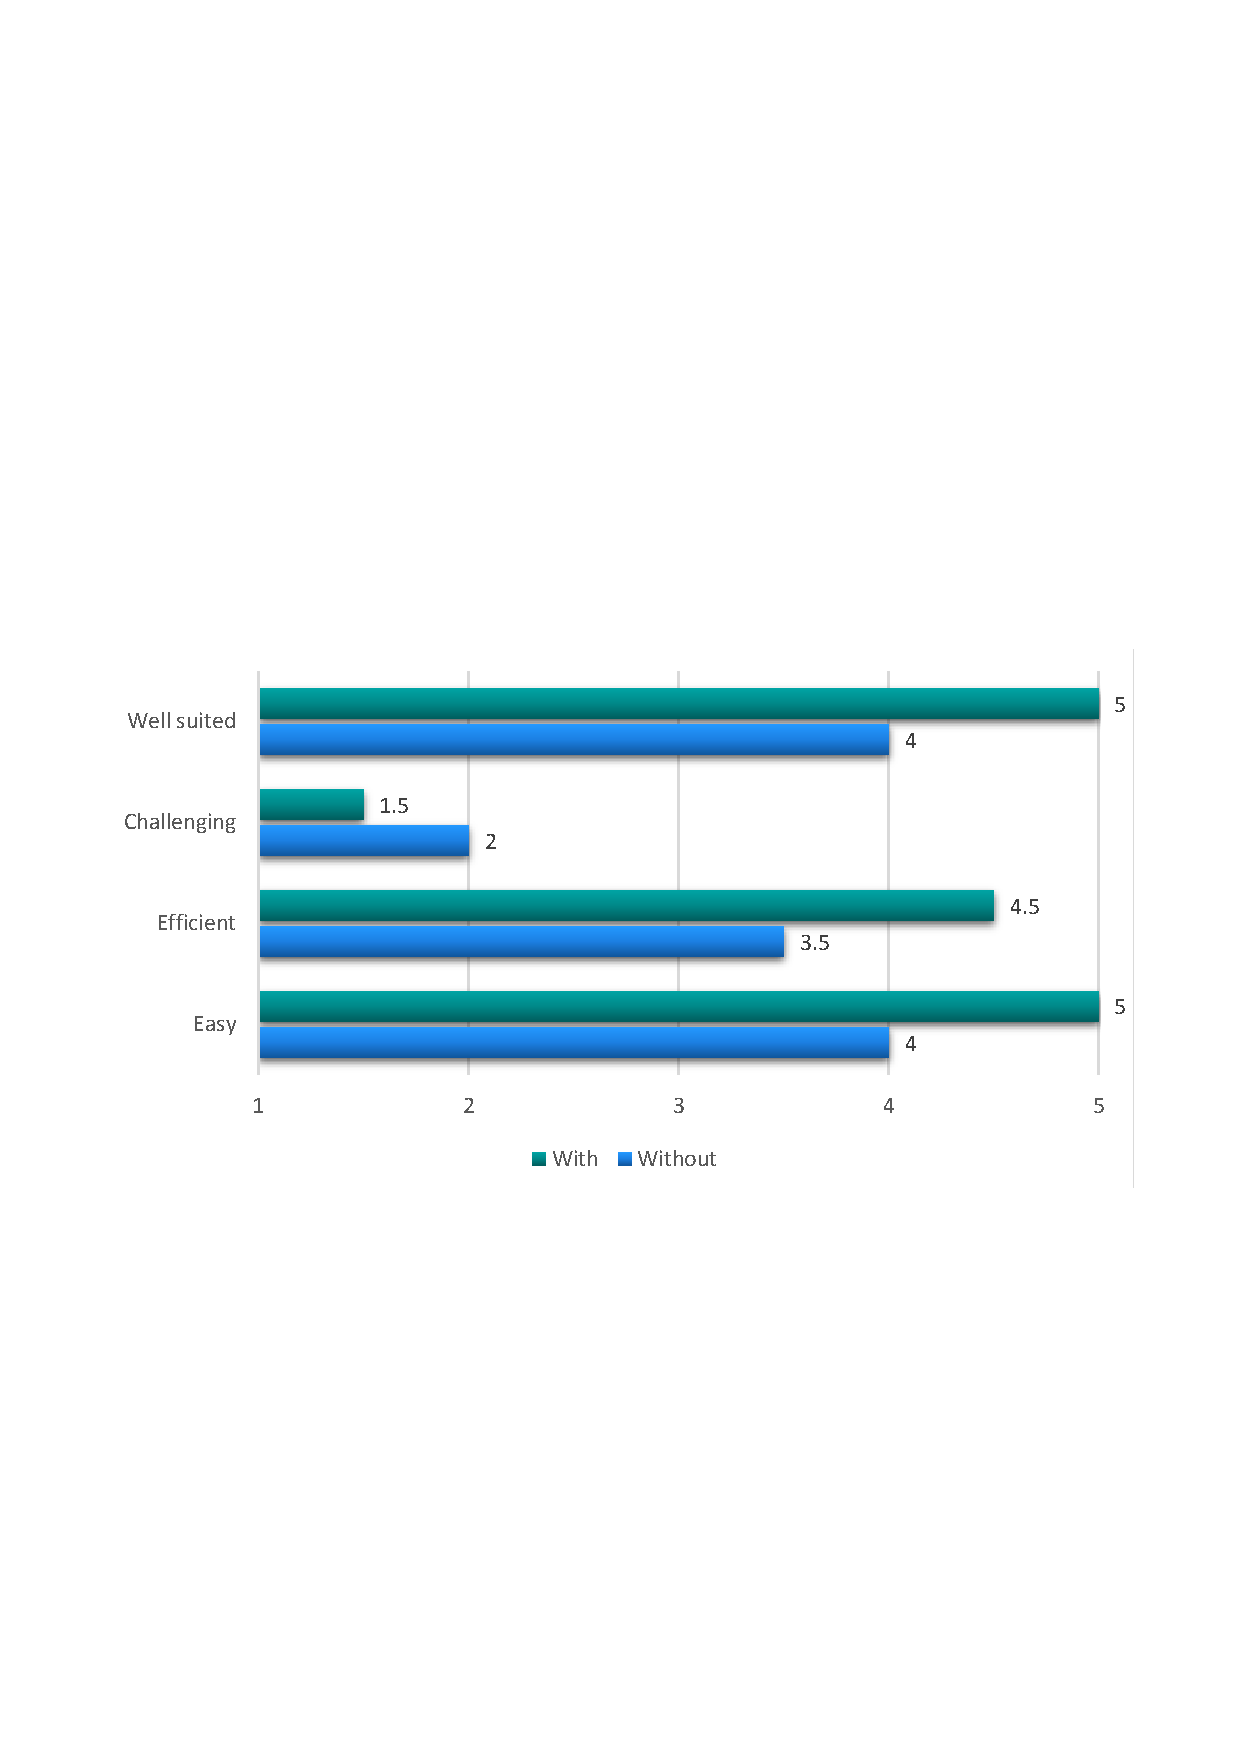
\includegraphics[width=0.8\textwidth]{images/charts/xdc_impl_comparison.pdf}
	\caption[xdc-impl: Comparison]{XDCinema implementation task - Comparison}
	\label{fig:xdc_impl_comparison}
\end{figure}

Figure~\ref{fig:xdc_impl_features_used} again shows the use and the ratings of the individual features. Again, no participant used the real devices. All participants used device emulation and the connection features and in contrast to the debugging task in XDCinema, device emulation was rated as very useful by all participants. Function debugging was used a bit less than in the debugging task, but the shared JavaScript console was used much more. It makes sense that function debugging is used more when fixing a bug; if one implements a feature and it works immediately when testing it, there is no need to debug a function, but if one has to fix a bug, there obviously must be a bug in a function and thus it makes much more sense to debug functions. The shared JavaScript console was rarely used to send commands and most participants did not use logging for solving the task, but many participants had some syntax errors when first testing the feature and noticed the error messages in the console. This also explains why the console was used more in the implementation task than in the debugging task: Generally, console outputs are very useful for debugging, but in this specific bug, there were no errors in the console in contrast to the implementation task, where syntax errors were shown in the console. Finally, the CSS editor was also used by some participants in this task. However, some completed the CSS part of the task using only the CSS file. This may be because they did not think of the CSS editor at this specific moment, or because they know CSS so well that they can just write everything down immediately, or also because they do not consider the CSS editor useful for this task.

\begin{figure}[H]
  \centering
    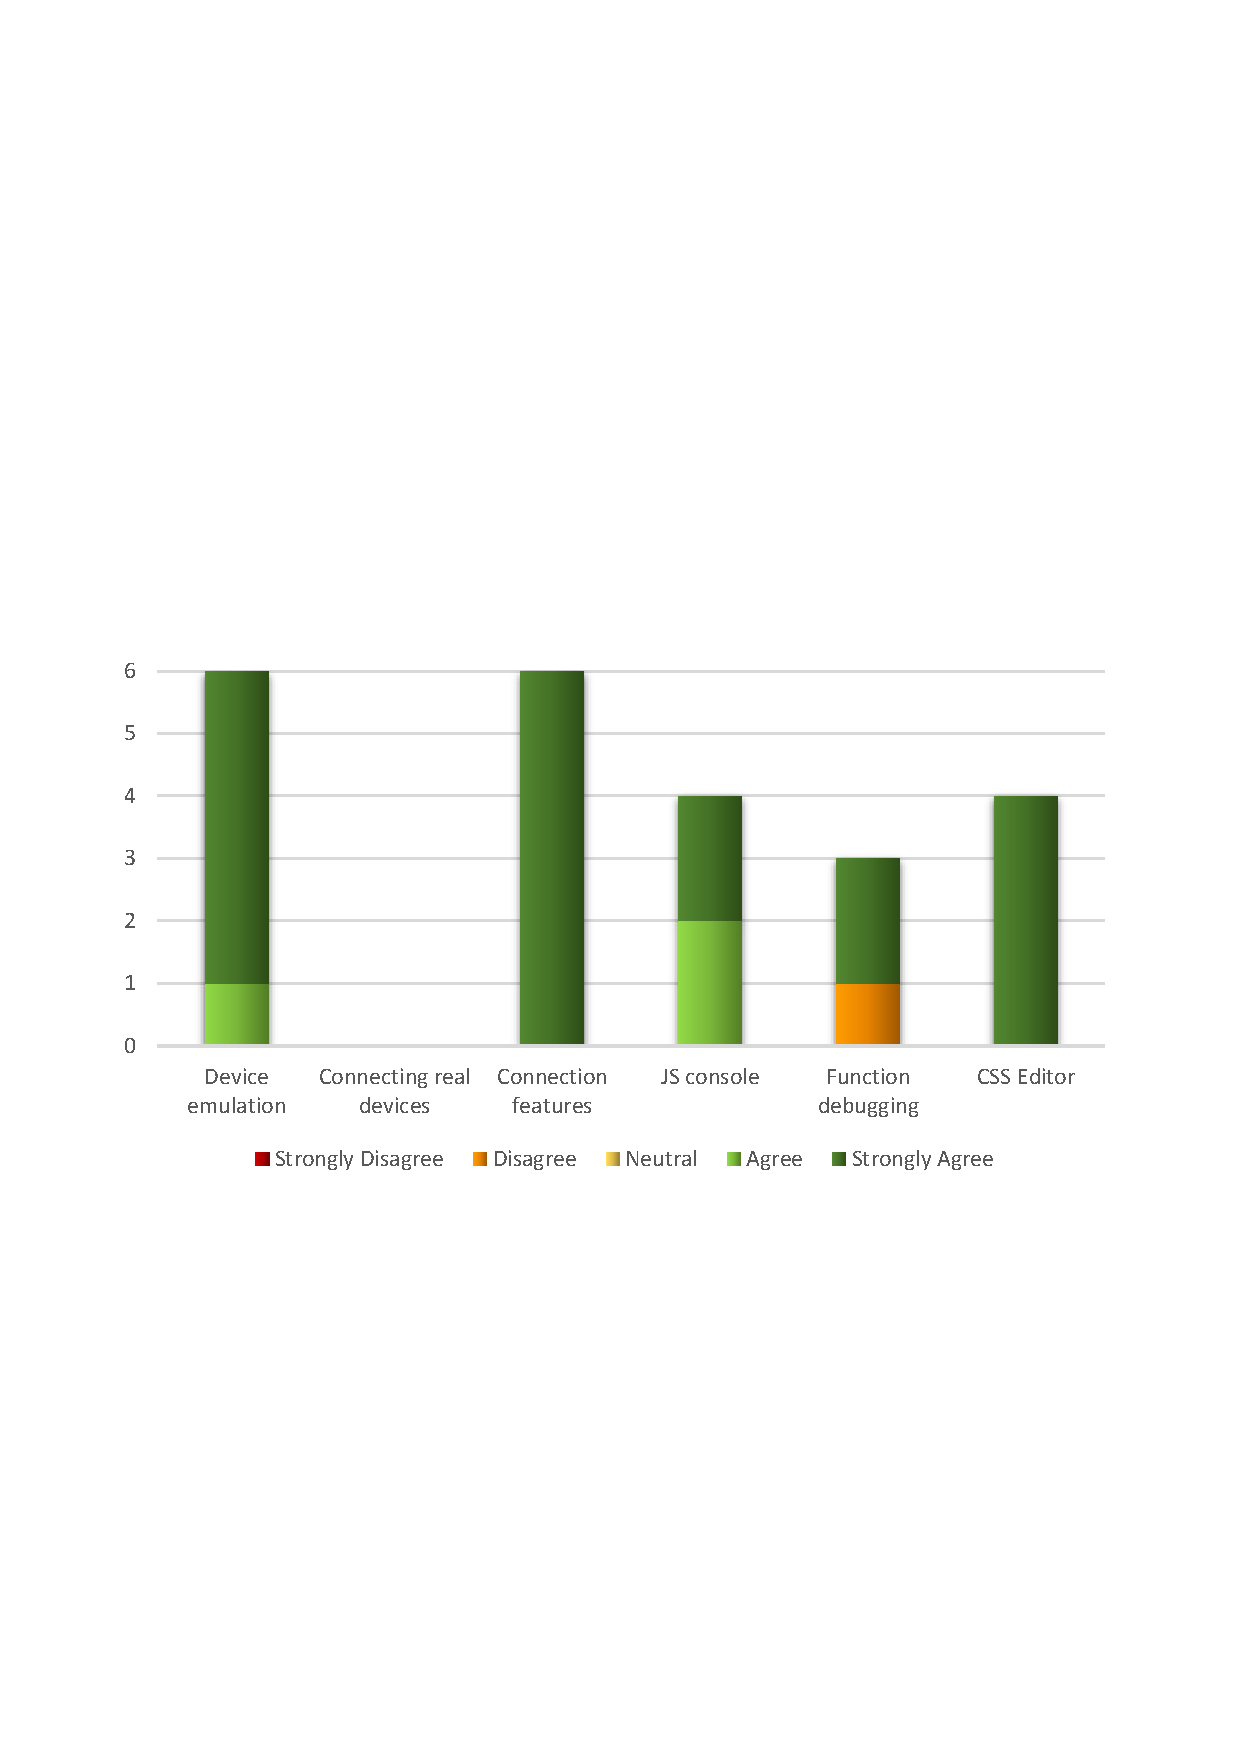
\includegraphics[width=0.8\textwidth]{images/charts/xdc_impl_features_used.pdf}
	\caption[xdc-impl: Features used]{XDCinema implementation task - Features used}
	\label{fig:xdc_impl_features_used}
\end{figure}

\subsection{XDYouTube: Fixing a Bug}

Figure~\ref{fig:xdyt_bug_comparison} shows the results for the debugging task in XDYouTube. The difference in suitability between our tools and the usual browser tools was most significant in this task with a difference of 2. The difference in efficiency is also rather large. Surprisingly, the task was rated as almost equally easy and challenging with and without our tools despite the large differences in the other questions. It seems that for this task, our tools did not make the task any easier to solve, but the participants felt more efficient when completing it. During the study, we noticed that most participants had problems reproducing the bug and almost all participants required some hints and finished the task more or less around the time limit. This could explain why the task was perceived as equally difficult with and without our tools: The participants did not really find the bug without help anyway, independent of whether they had access to our tools, so it makes sense that they would consider the task as difficult in general. 

\begin{figure}[H]
  \centering
    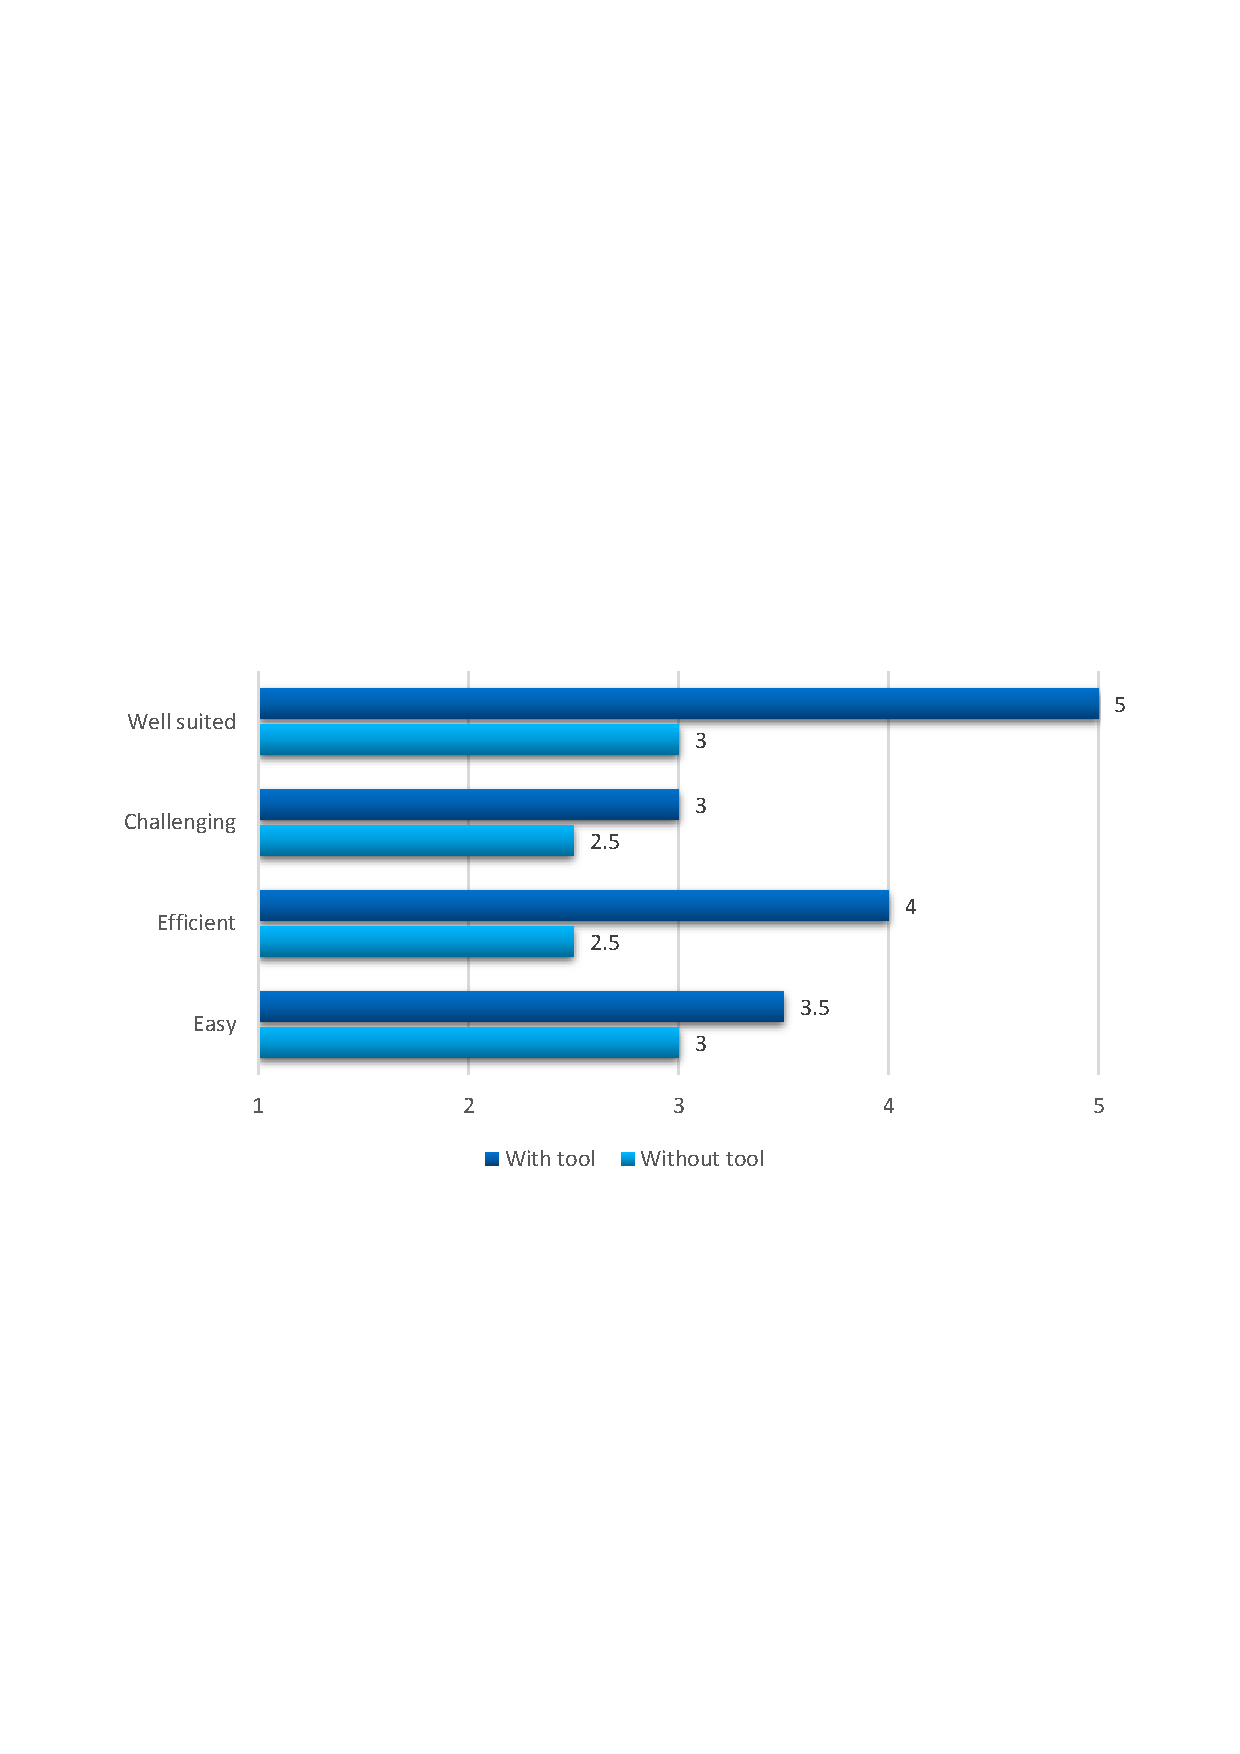
\includegraphics[width=0.8\textwidth]{images/charts/xdyt_bug_comparison.pdf}
	\caption[xdyt-bug: Comparison]{XDYouTube debugging task - Comparison}
	\label{fig:xdyt_bug_comparison}
\end{figure}

In Figure~\ref{fig:xdyt_bug_features_used}; the use and ratings of the individual features can be seen. All of the participants used device emulation and connection features and rated them as useful. Function debugging was also used by almost all participants, probably because it was difficult to reproduce the bug and the participants wanted to see what was going on in the functions. About half the participants used the shared JavaScript console, mainly to see the error produced in the function that caused the bug. One participant connected the Nexus 7 to our tools and liked the feature, but no statement about the general usefulness of the feature can be made from just one participant. 

\begin{figure}[H]
  \centering
    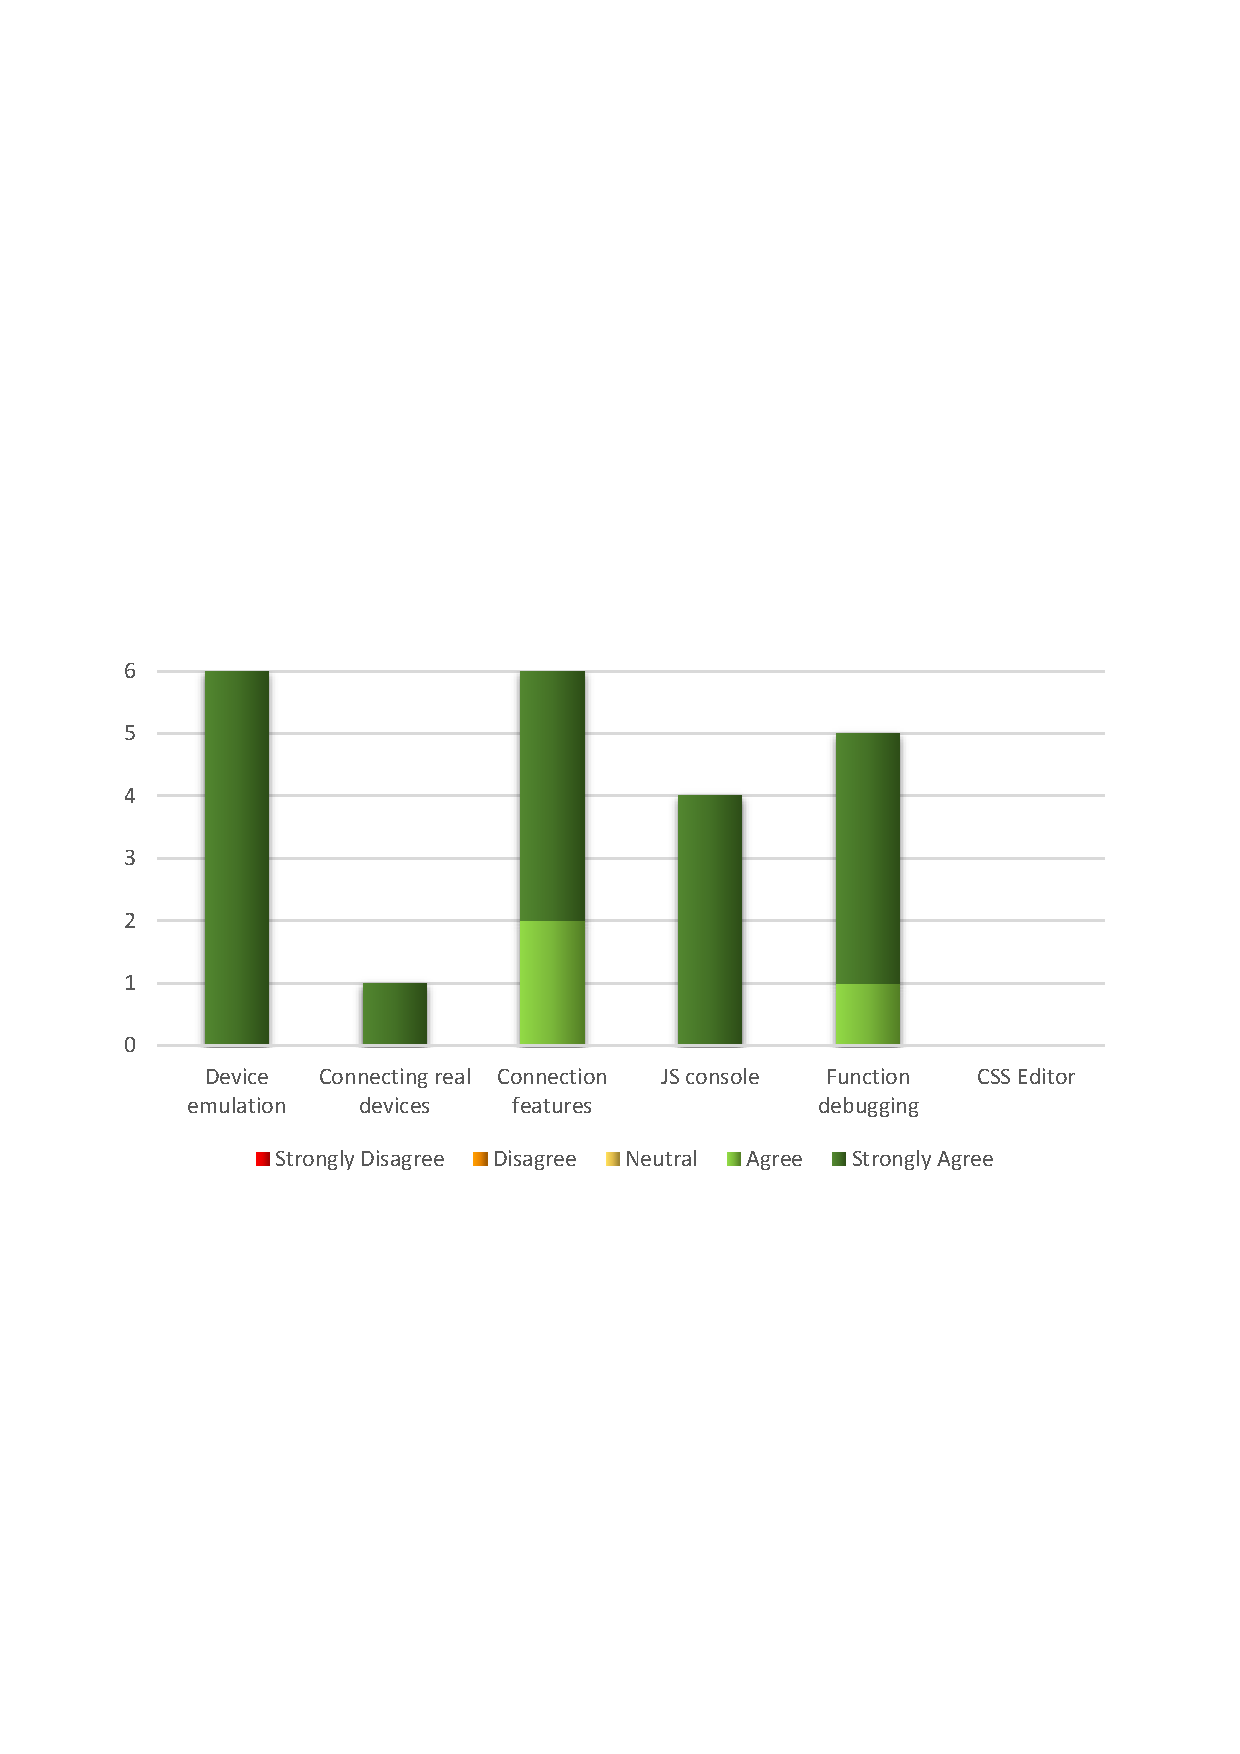
\includegraphics[width=0.8\textwidth]{images/charts/xdyt_bug_features_used.pdf}
	\caption[xdyt-bug: Features used]{XDYouTube debugging task - Features used}
	\label{fig:xdyt_bug_features_used}
\end{figure}

\subsection{XDYouTube: Implementing a Feature}

Figure~\ref{fig:xdyt_impl_comparison} shows the results for the implementation task in XDYouTube. In this task, all questions were clearly rated in favor of our tools. While the participant answered the questions in a rather neutral way when they did not have access to our tools, they clearly stated that the task was easy to complete and felt efficient to complete with our tools. This task differs from the others a bit, because all other tasks had questions where the difference in median was 0.5 or 0, whereas the difference is at least 1 in this task for every question. Especially in the questions concerning how challenging and how easy it was to complete a task, a big difference to the other three tasks can be seen. For the other three tasks, the difference between how challenging the task was was 0.5 for all tasks, and ranged from 0 to 1 regarding how easy it was to complete the task. In this task, the difference was 1.5 for both questions. Thus, this seems to be the only task where our tools made the task much easier to complete. One participant mentioned that they think that the XDYouTube tasks were better suited for the study because they emphasize the cross-device scenario more. If the other participants felt the same way about the task, this could be a possible explanation why they profited the most from our tools in this task.

\begin{figure}[H]
  \centering
    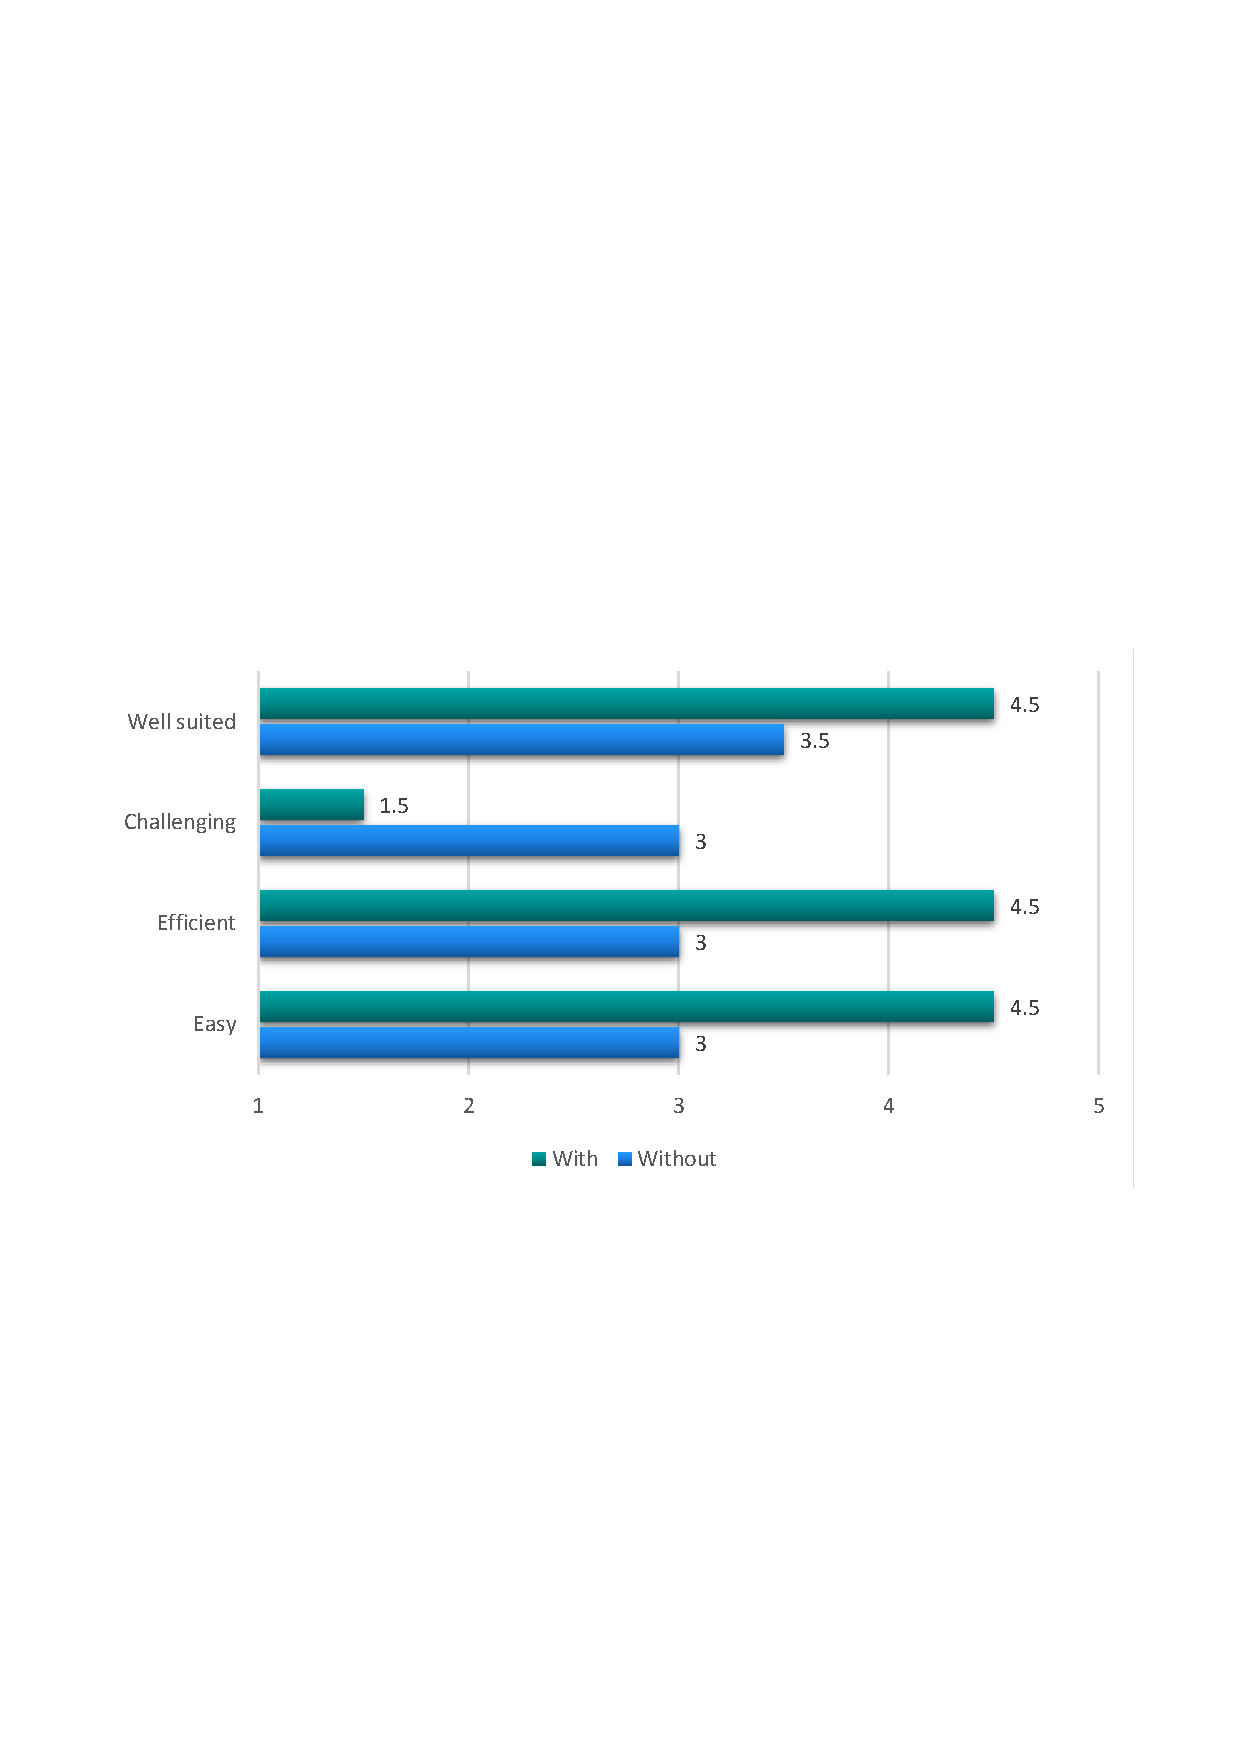
\includegraphics[width=0.8\textwidth]{images/charts/xdyt_impl_comparison.pdf}
	\caption[xdyt-impl: Comparison]{XDYouTube implementing task - Comparison}
	\label{fig:xdyt_impl_comparison}
\end{figure}

In Figure~\ref{fig:xdyt_impl_features_used}; the use and ratings of the individual features can be seen. Once again, device emulation and the connection features were used by every participant. The shared JavaScript console and CSS editor were about equally popular and rated as very useful except for one participant that had a neutral opinion on the console. Function debugging was rarely used for this task. This is rather surprising because many participants had a bug where they had switched playing and pausing the video at the beginning and this could probably have been solved easily by debugging the function. However, most participants just got stuck at the bug and required some hints to fix it instead of debugging their functions.

\begin{figure}[H]
  \centering
    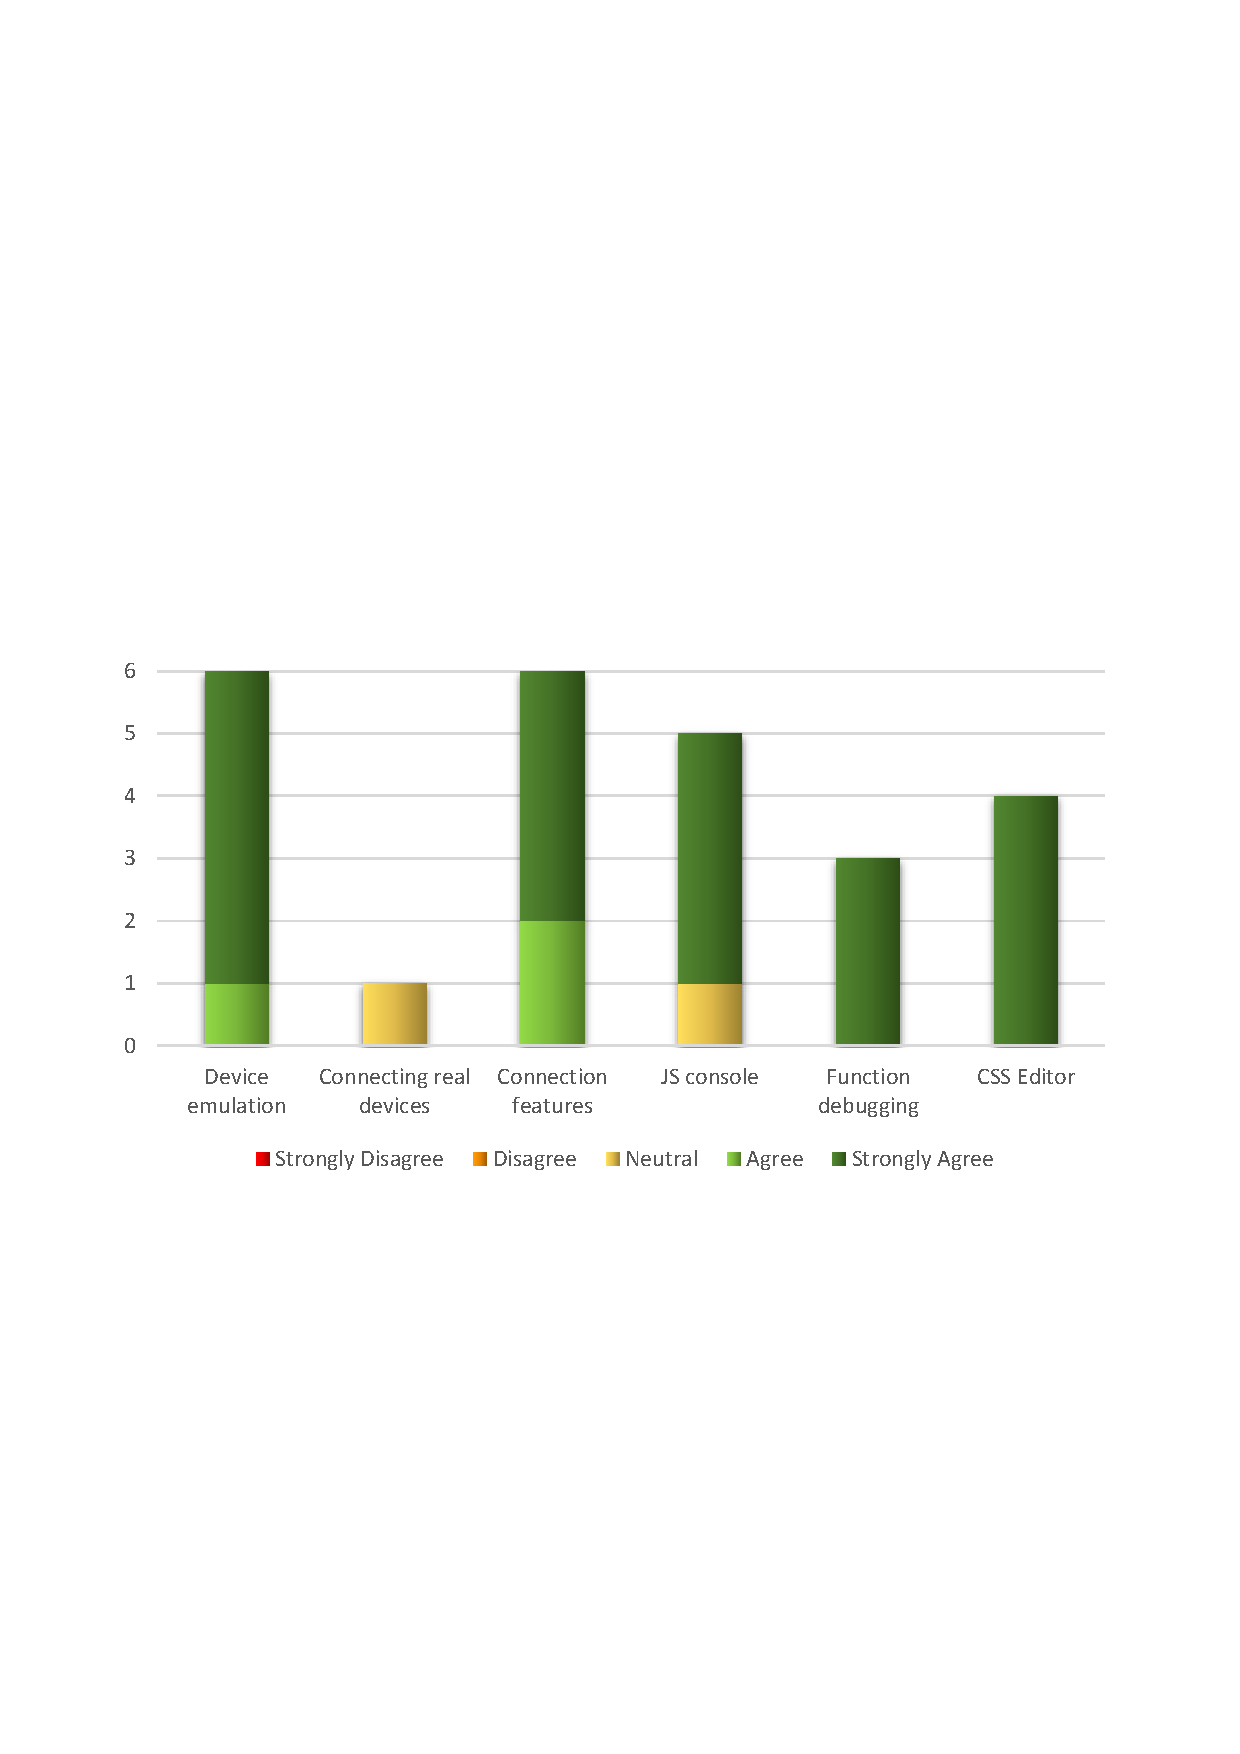
\includegraphics[width=0.8\textwidth]{images/charts/xdyt_impl_features_used.pdf}
	\caption[xdyt-impl: Features used]{XDYouTube implementing task - Features used}
	\label{fig:xdyt_impl_features_used}
\end{figure}

\subsection{General}

In general, our tools were rated as very well suited for all tasks with a median value of 5 for each task except the XDYouTube implementation task where the median value is 4.5. In contrast, the usefulness of the usual browser tools was rated with median values between 3 and 4, this indicates that our tools are indeed better suited for implementing and debugging cross-device applications. The efficiency was also rated as significantly better for all tasks except the debugging task in XDCinema, where the difference was only 0.5. This indicates that our tools make the process of testing cross-device applications more efficient. The difference in easiness seems to depend partially on the type of task; in the tasks where the participants had to implement a feature, completing the task with our tools was clearly considered easier, whereas the difference was smaller for the tasks where the participants had to fix a bug. Surprisingly, the results for the question about how challenging it was to complete the task do not necessarily relate to the results of the question about easiness. For all tasks except the XDYouTube implementation task, the differences are very minor, thus our tools do not seem to have much influence on how challenging a task is perceived.

Without our tools, it looks like participant considered the XDYouTube tasks as more difficult than the XDCinema tasks. This generally corresponds to what participants said during the study. While most of them did not make any comments about the difficulty of the task, those who did said that the XDYouTube tasks were more difficult. However, when using our tools, the picture looks a bit different. With access to our tools, it seems that the debugging tasks are considered harder than the implementation tasks. In principle, this is the opposite of what we wanted to achieve, as the debugging tasks were designed as "introduction" tasks. However, the completion times show that the participants were not actually faster when completing the implementation tasks than when completing the debugging tasks, therefore the different results in the questionnaires can be considered as okay. Surprisingly, the difference in median values for the question where we asked how well suited the tools were for the tasks is larger in the debugging tasks than in the implementation tasks. The difference is 1 for both implementation tasks and 1.5 and 2 for the debugging tasks. Thus, the participants that had access to our tools considered the debugging tasks as more difficult than the implementation tasks, but still felt that our tools were much better suited than the usual browser tools. So far, those results make sense: If the task is more difficult, the user can profit more from our tools. However, what remains to be explained is why the participants that did not have access to our tools found the XDYouTube tasks more difficult than the XDCinema task. The explanation lies in the XDYouTube implementation task: As mentioned before, participants seem to profit the most of our tools in this tasks. Consequently, our tools make the task so much easier that it is no longer considered one of the more difficult tasks by the participants that have access to our tools. However, the XDCinema bug was not really perceived as easier to complete with our tools, thus it is one of the more challenging tasks for the participants that had access to our tools, but not for the participants that did not have access to our tools.

\section{Discussion}

Figure~\ref{fig:implementing_easier} shows that about three quarters of all participants considered implementing a feature easier with our tools. Only one participant found it easier to implement a feature without our tools. However, in principle, this option is redundant as the participants still have access to the browser tools even when they have access to our tools. Thus the relevant conclusion is that about one quarter of the participants did not see any gain in easiness from using our tools. The same applies to the question about whether implementing a feature feels more efficient with our tools (see Figure~\ref{fig:implementing_efficient}); this figure shows exactly the same results as the figure about easiness. However, all except one participant preferred implementing a feature with our tools (see Figure~\ref{fig:prefer_implementing}). Thus, it seems that participants like to have access to our tools even if they cannot directly relate them to a decrease in difficulty or to an increase in efficiency.
\begin{figure}[H]
  \centering
    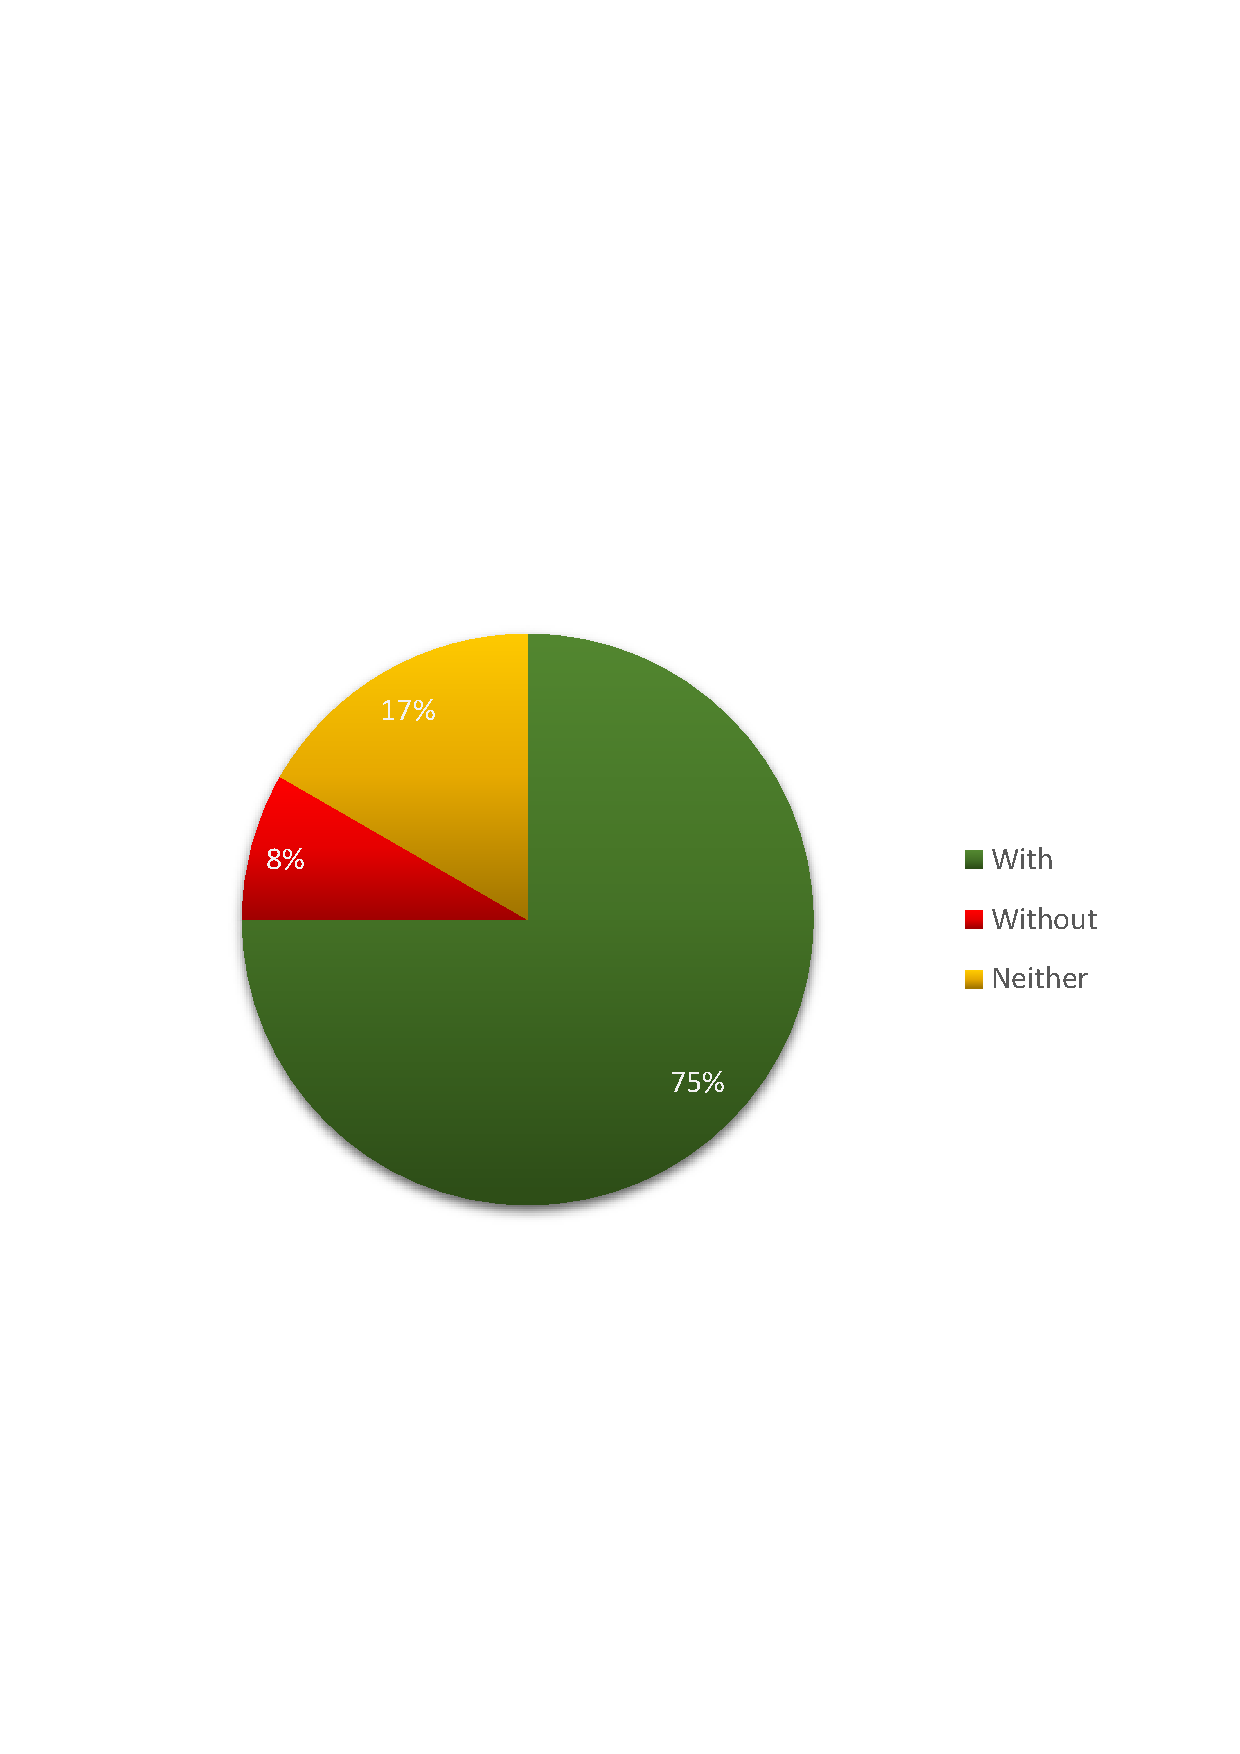
\includegraphics[width=0.6\textwidth]{images/charts/implementing_easier.pdf}
	\caption[Easiness of implementing]{Easiness of implementing a feature}
	\label{fig:implementing_easier}
\end{figure}

\begin{figure}[H]
  \centering
    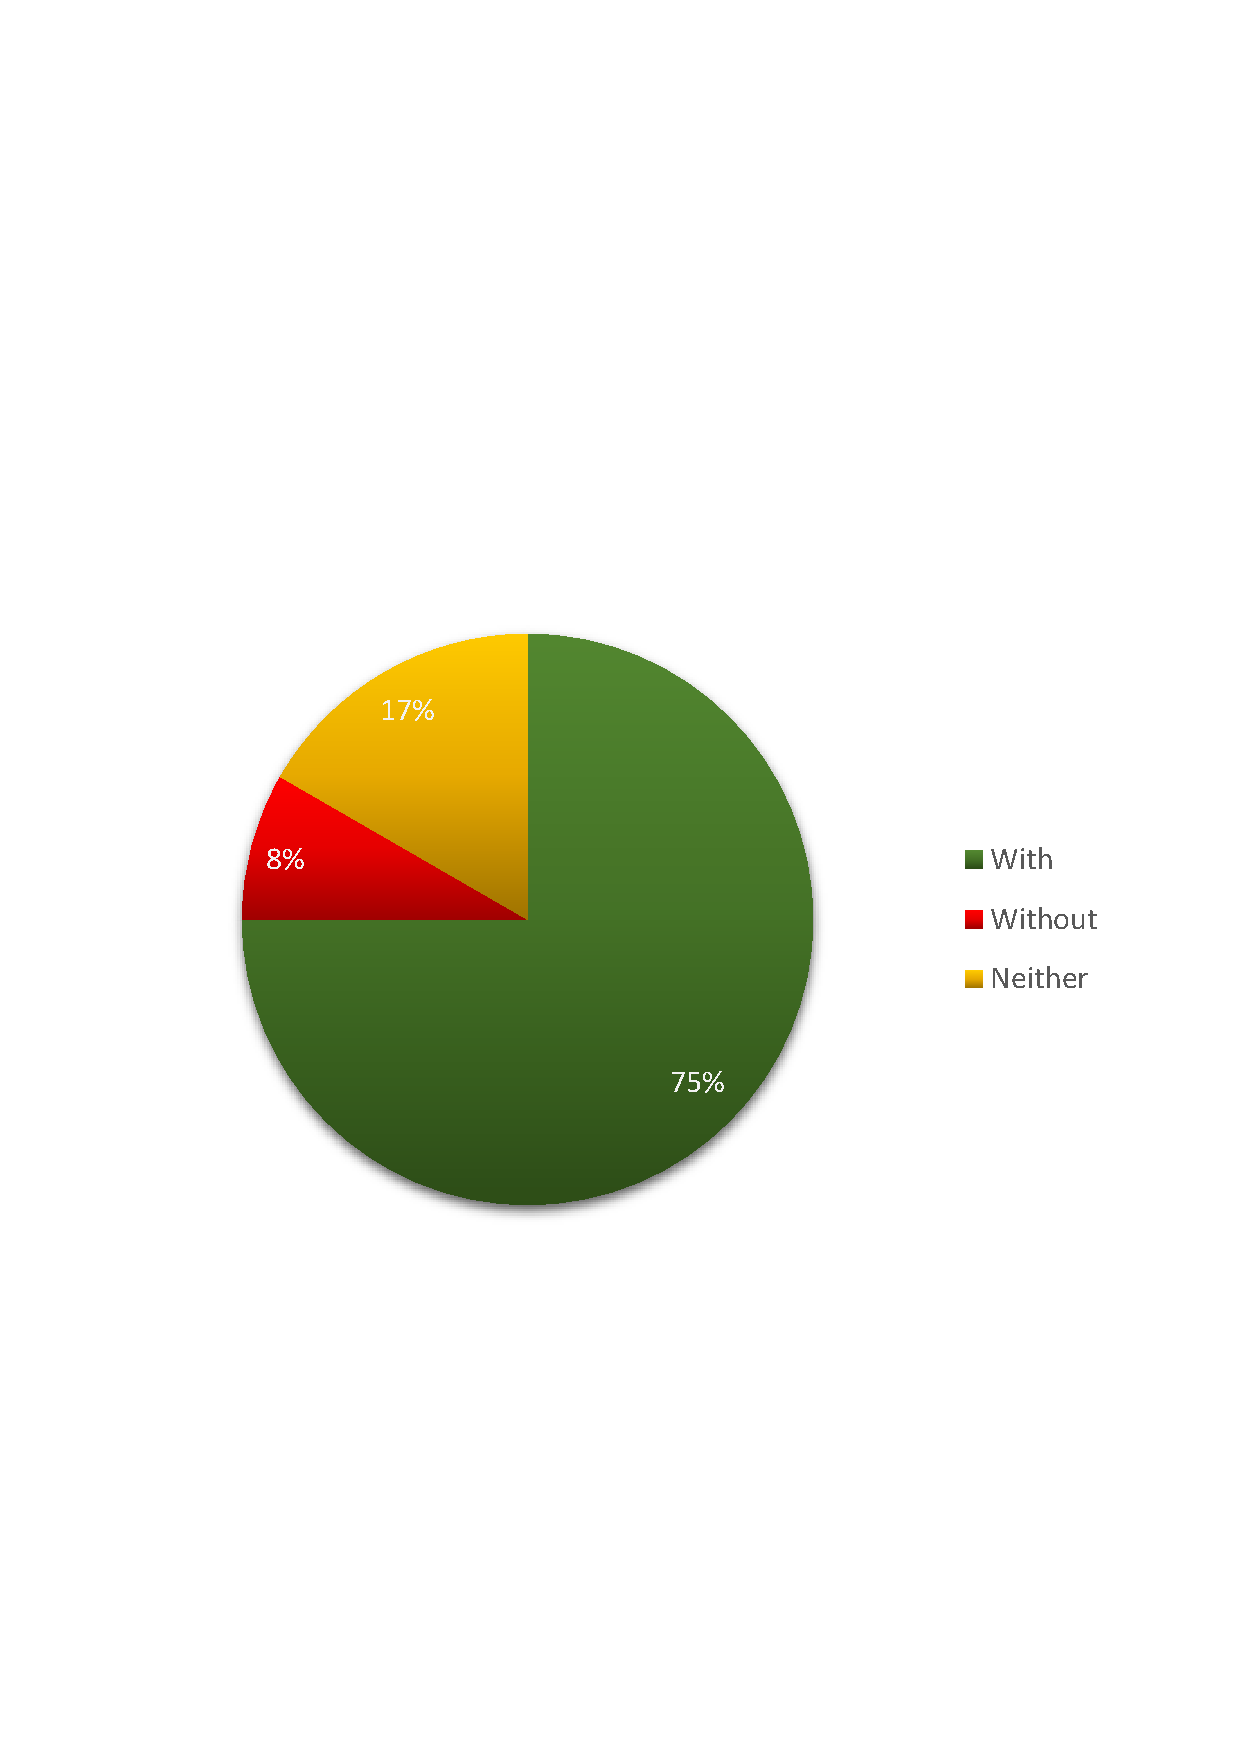
\includegraphics[width=0.6\textwidth]{images/charts/implementing_efficient.pdf}
	\caption[Efficiency of implementing]{Efficiency of implementing a feature}
	\label{fig:implementing_efficient}
\end{figure}

\begin{figure}[H]
  \centering
    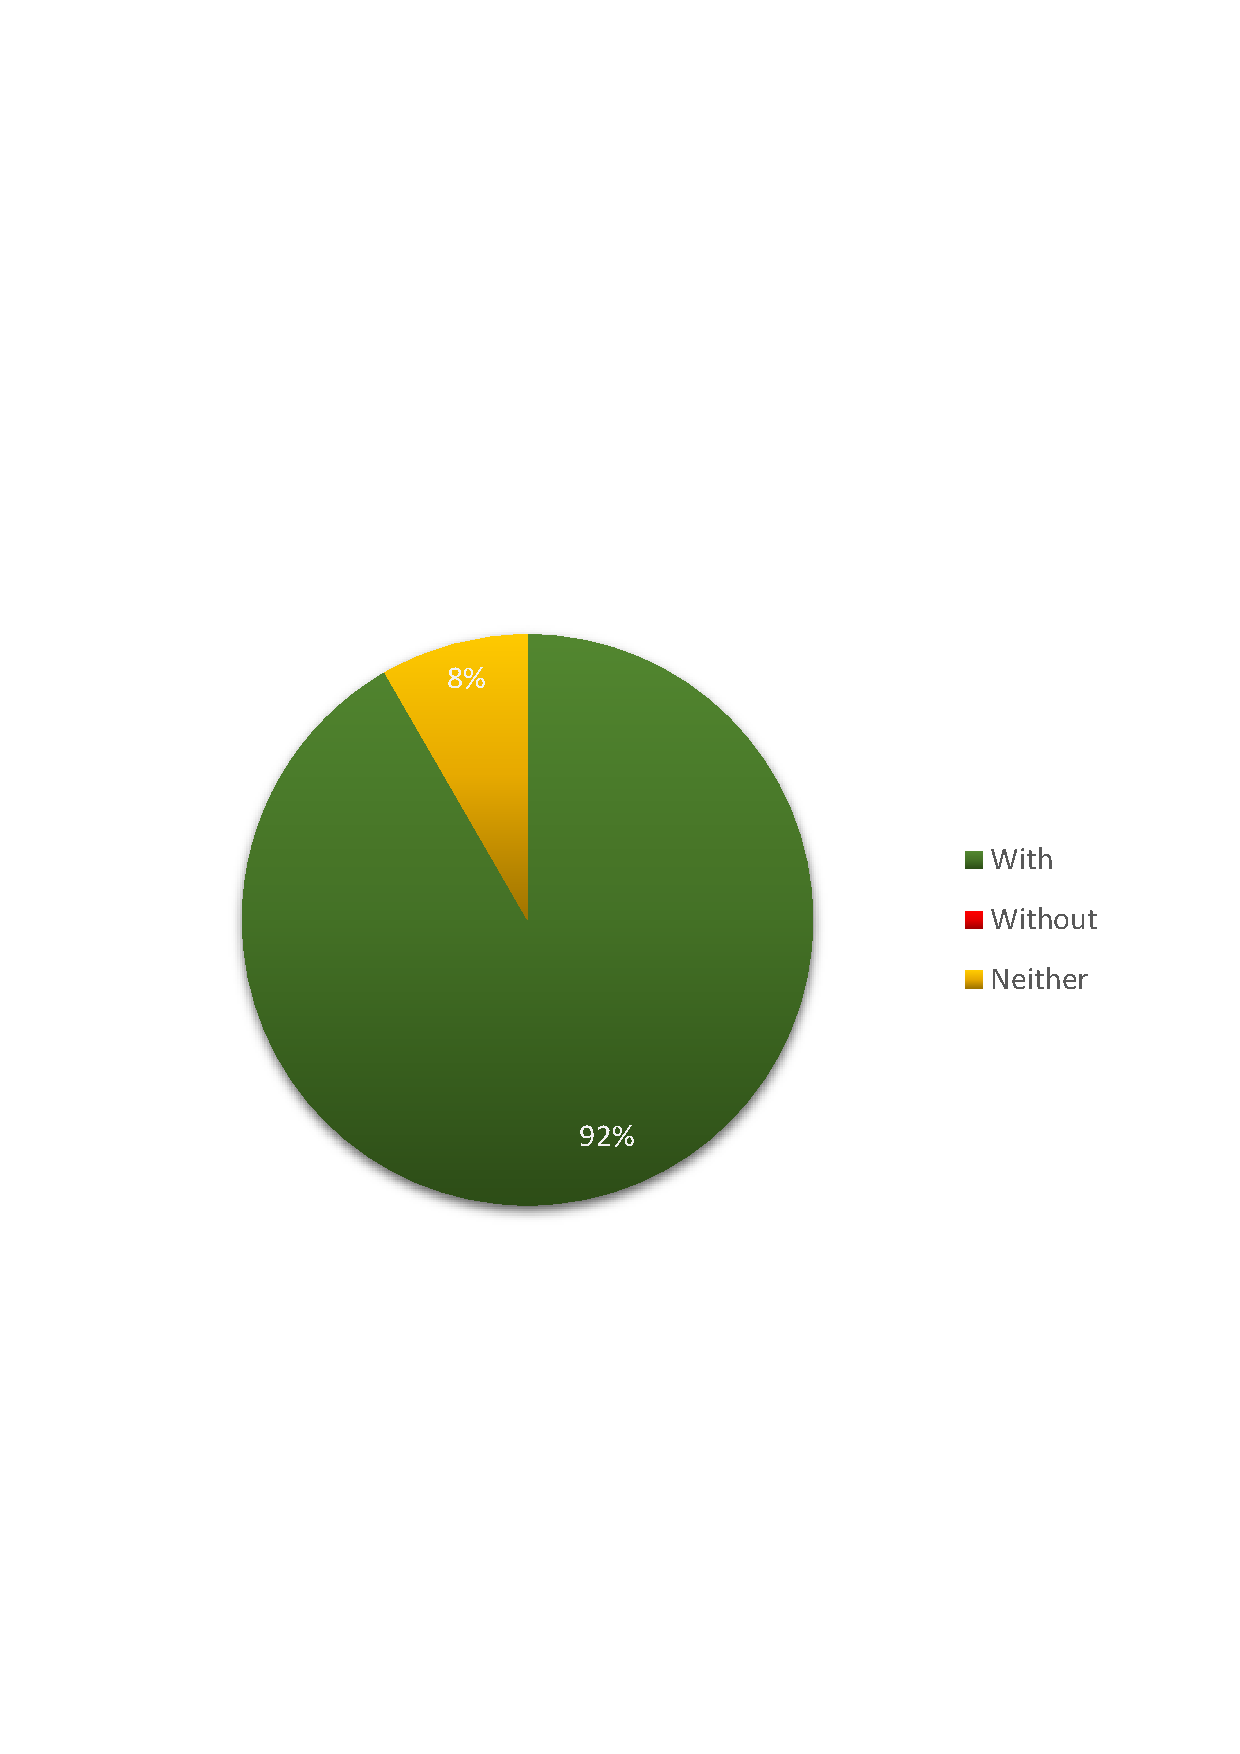
\includegraphics[width=0.6\textwidth]{images/charts/prefer_implementing.pdf}
	\caption[Preference for implementing]{Preference for implementing a feature}
	\label{fig:prefer_implementing}
\end{figure}

Figure~\ref{fig:debugging_easier} shows that most participants found it easier to debug a cross-device application with our tools. The results get even more obvious if we look at Figure~\ref{fig:debugging_efficient} and Figure~\ref{fig:prefer_debugging}. Those two figures show that all participants felt more efficient when debugging with our tools and also preferred debugging with our tools.

\begin{figure}[H]
  \centering
    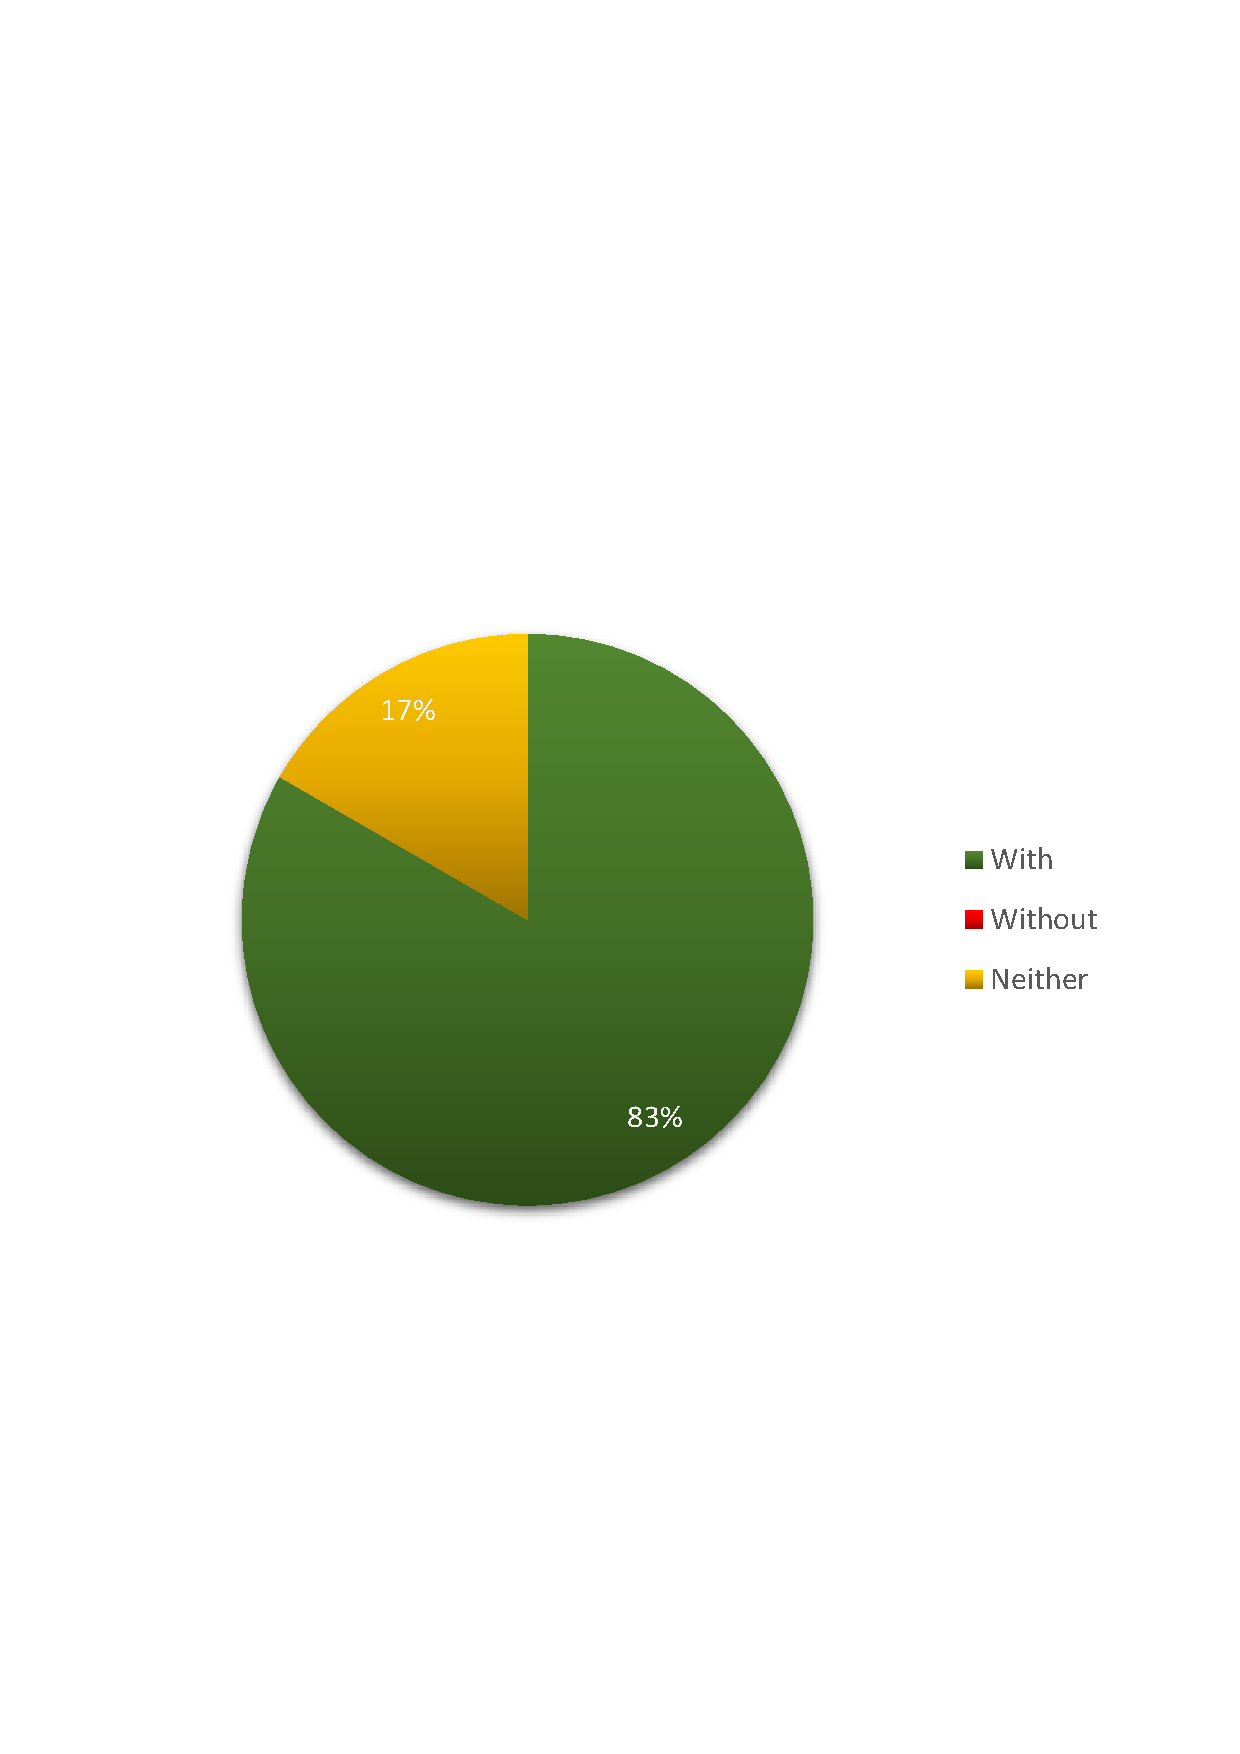
\includegraphics[width=0.6\textwidth]{images/charts/debugging_easier.pdf}
	\caption[Easiness of debugging]{Easiness of debugging}
	\label{fig:debugging_easier}
\end{figure}

\begin{figure}[H]
  \centering
    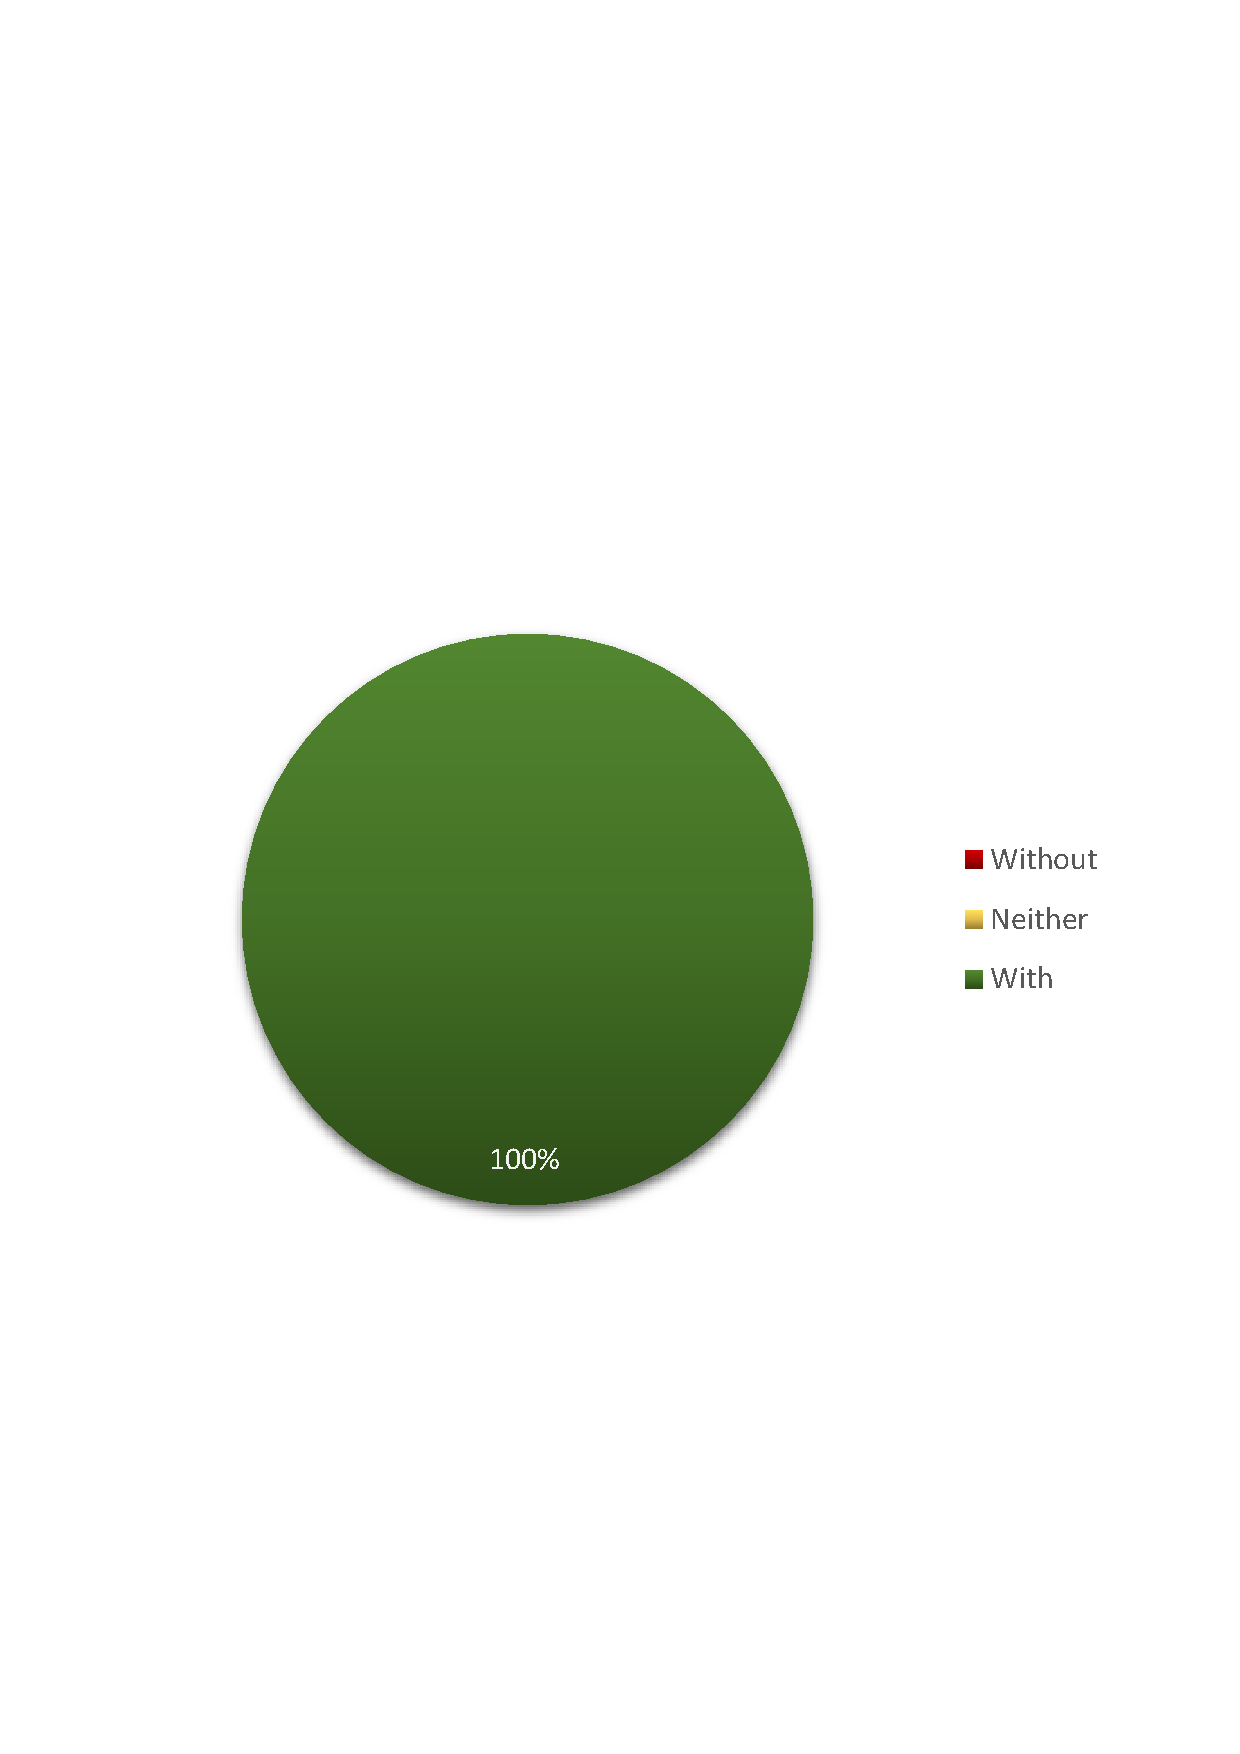
\includegraphics[width=0.6\textwidth]{images/charts/debugging_efficient.pdf}
	\caption[Efficiency of debugging]{Efficiency of debugging}
	\label{fig:debugging_efficient}
\end{figure}

\begin{figure}[H]
  \centering
    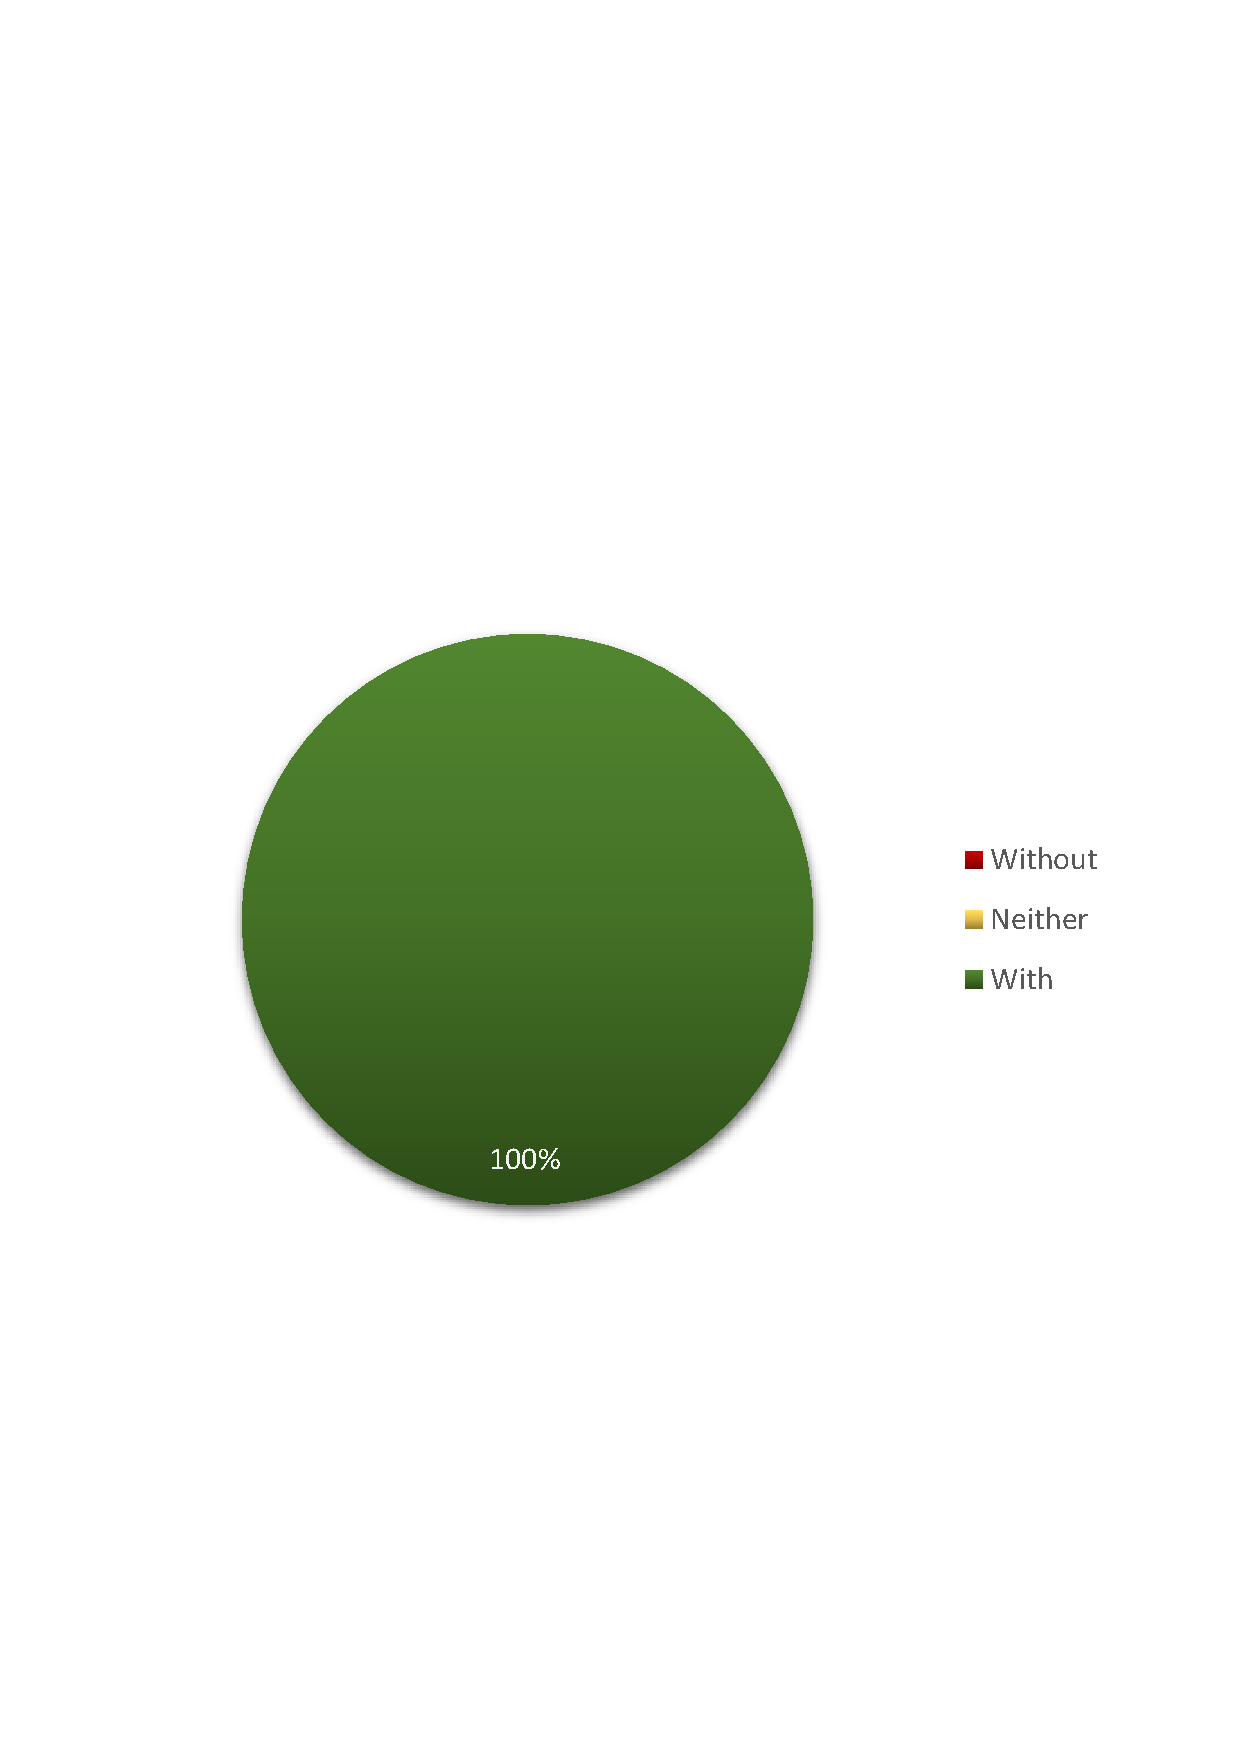
\includegraphics[width=0.6\textwidth]{images/charts/prefer_debugging.pdf}
	\caption[Preference for debugging]{Preference for debugging}
	\label{fig:prefer_debugging}
\end{figure}


We also asked the participants if they would use our tools for debugging and implementing cross-device applications and if they think that our tools would be useful for cross-device application testing. The results can be seen in figure~\ref{fig:usefulness_tool}. Almost all participants think that our tools would be very useful for implementing as well as debugging cross-device applications and the remaining few also think that they would be useful. All participants would use our tools for implementing cross-device applications and all except one participant would use them for debugging cross-device applications. A few more participants stated that they strongly agree with the statement that they would use our tools for debugging than for implementing. This is consistent with our previous results, where all participants preferred debugging with our tools but about one quarter did not prefer implementing with our tools.

\begin{figure}[H]
  \centering
    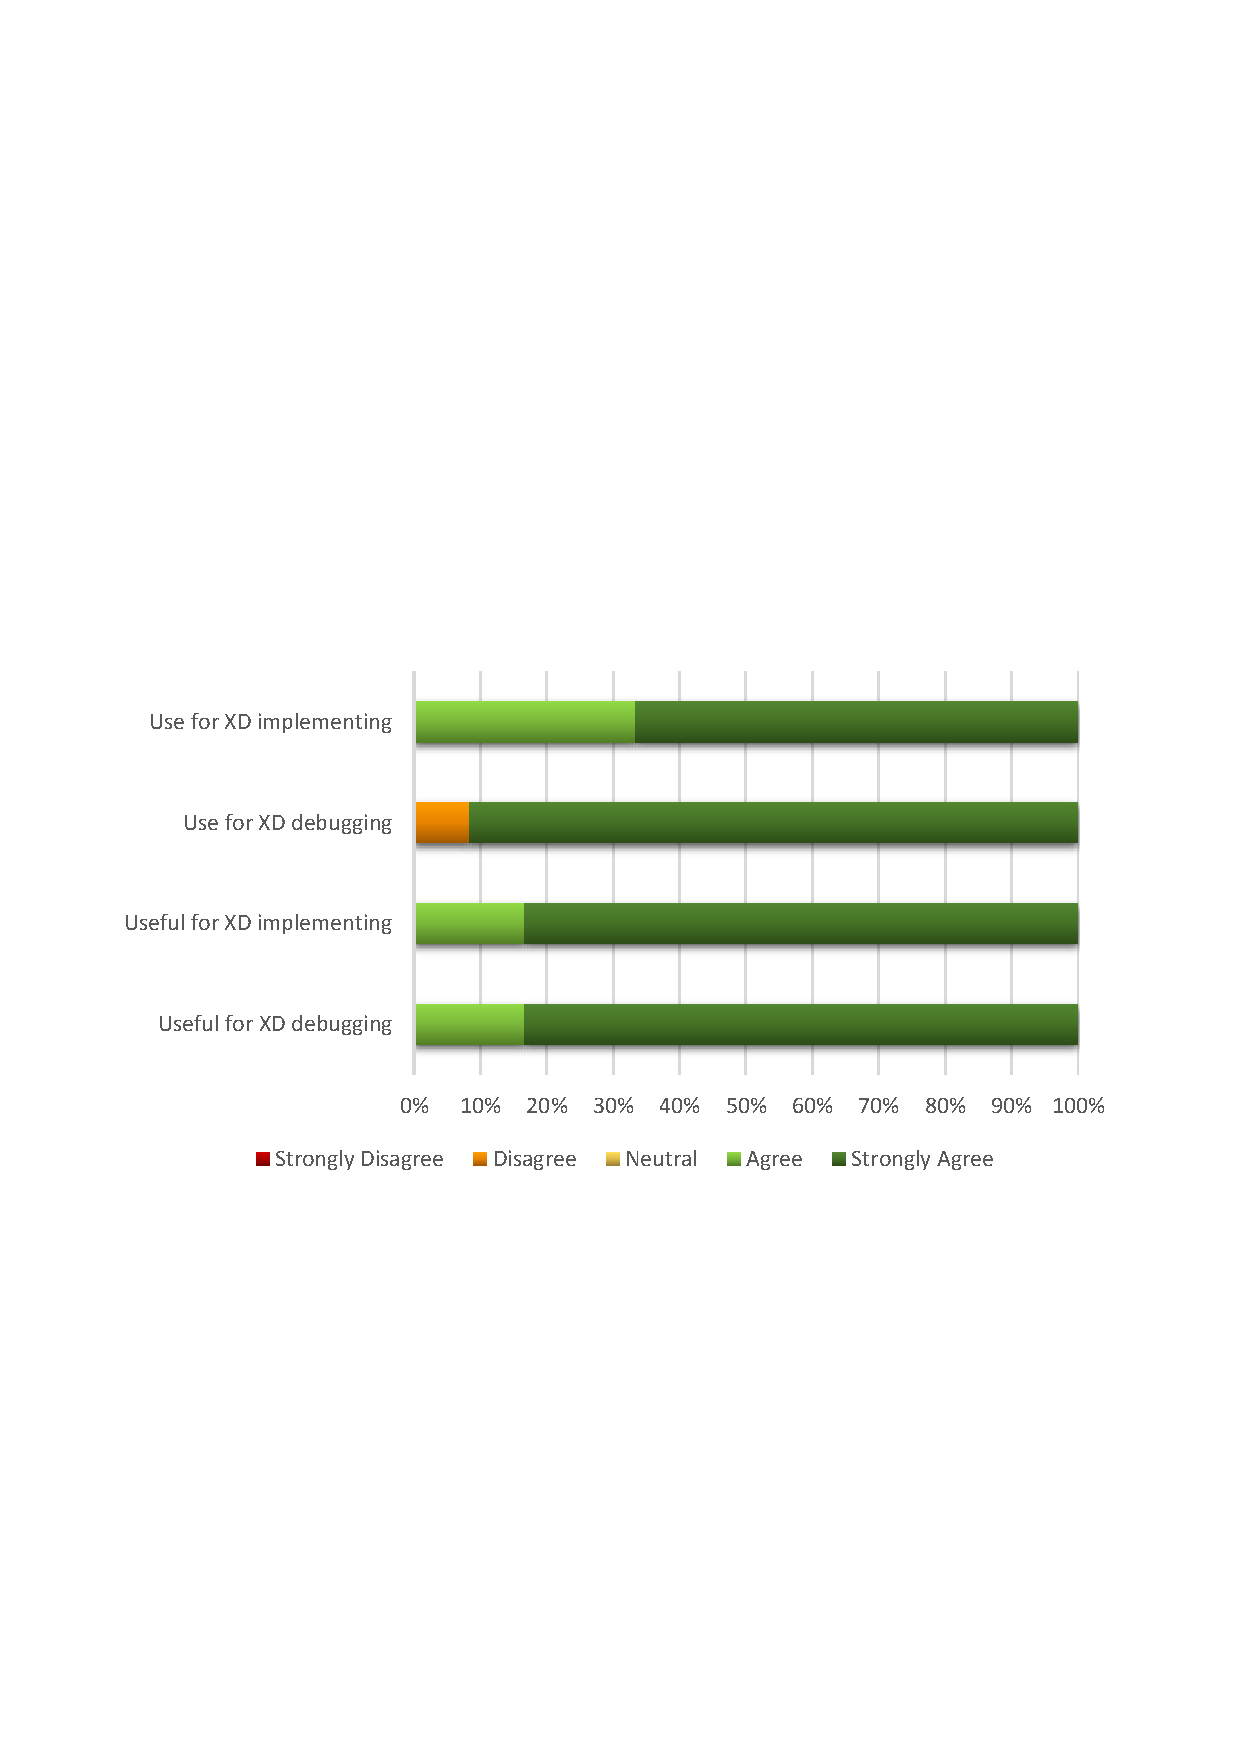
\includegraphics[width=0.8\textwidth]{images/charts/usefulness_tool.pdf}
	\caption[Usefulness]{Usefulness of our tools}
	\label{fig:usefulness_tool}
\end{figure}

Finally, you can see the results for the general questions about our tools in Figure~\ref{fig:tool_general}. The figure shows that our tools were perceived as easy to learn despite the many different features and the participants also felt rather confident using our tools. However, some participants rated the question about confidence in a neutral way and most other participants felt only somewhat confident, but not very confident. This indicates that even though our tools are considered easy to learn, it may still take participants some time to get used to them. Our tools are not considered as unnecessarily complex by almost all participants. The results of those three questions indicate that the interface of our tools is generally well-structured and it would be easy for developers to get used to our tools.

\begin{figure}[H]
  \centering
    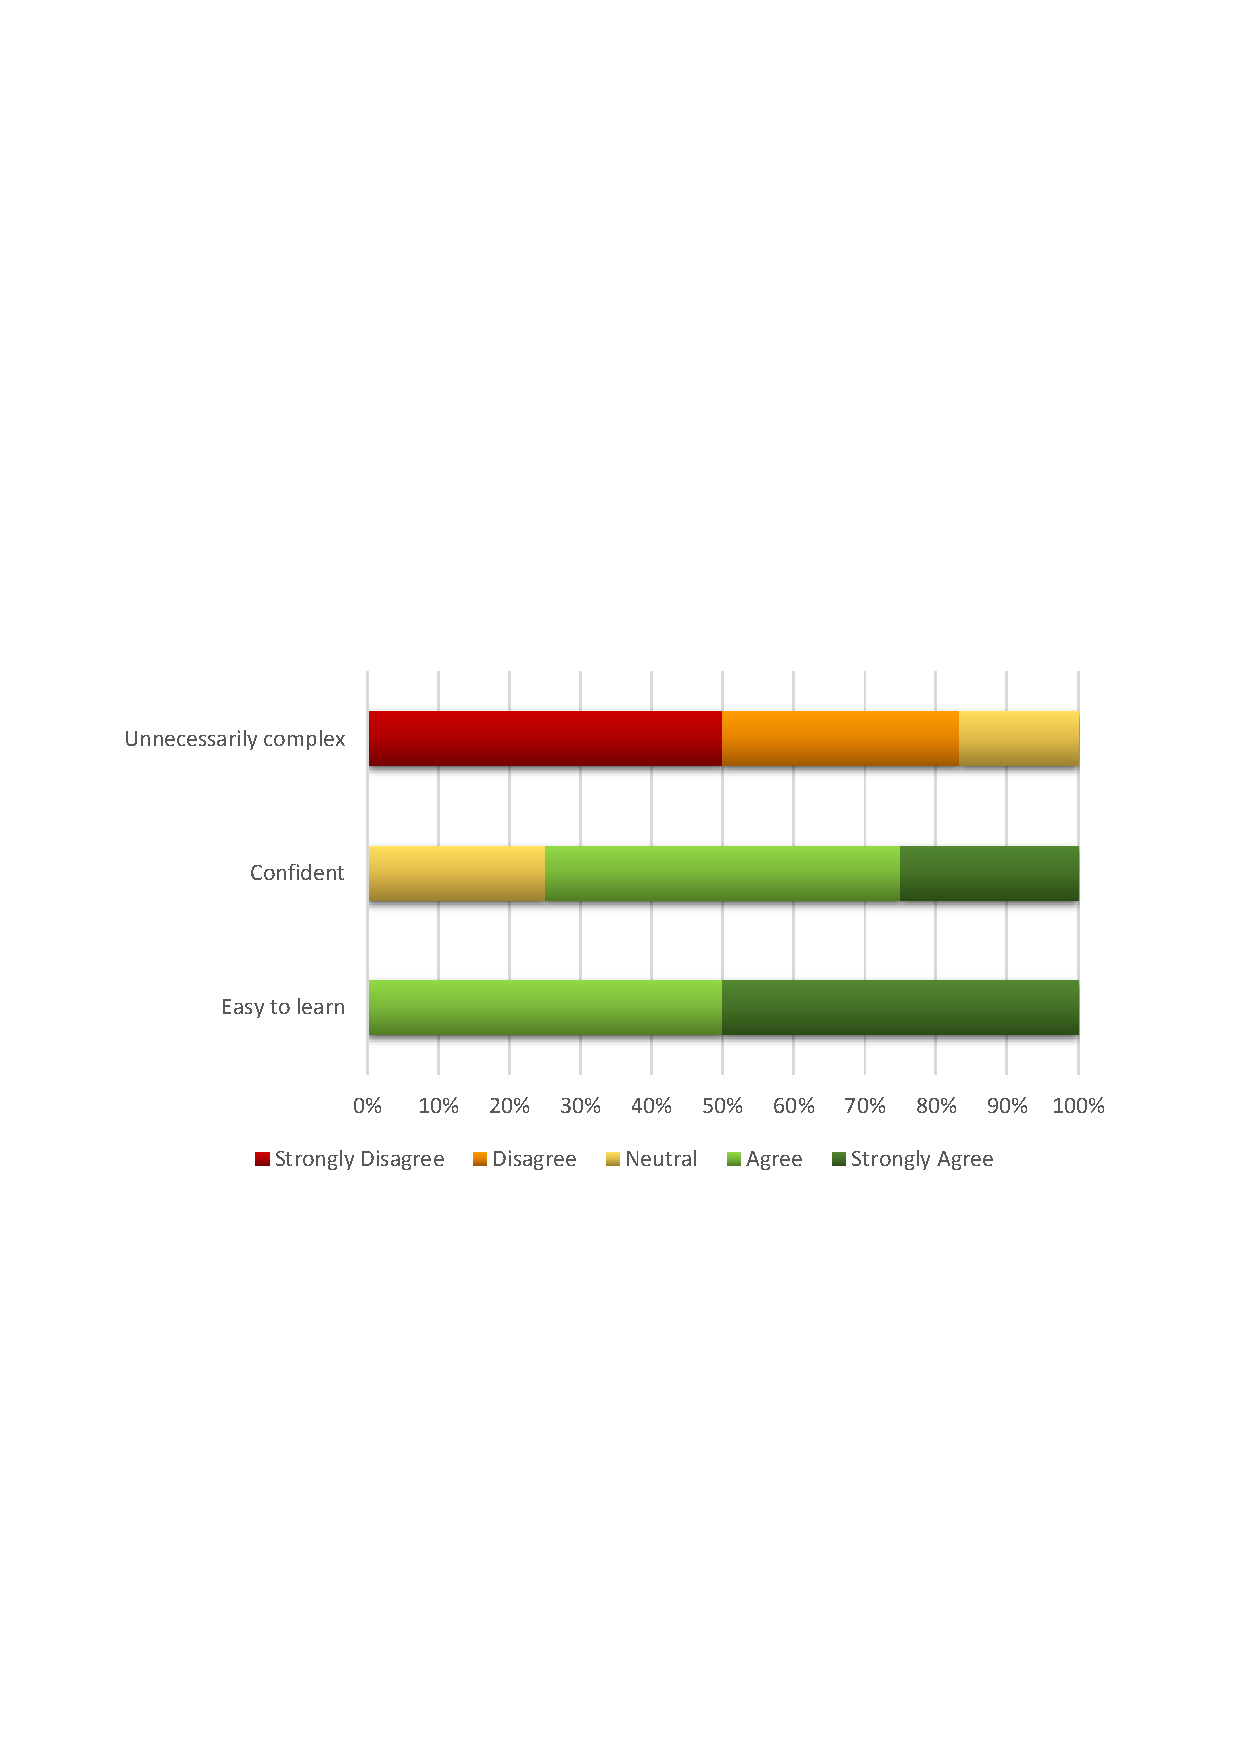
\includegraphics[width=0.8\textwidth]{images/charts/tool_general.pdf}
	\caption[General Evaluation]{General evaluation of our tools}
	\label{fig:tool_general}
\end{figure}

Figure~\ref{fig:would_use_features} shows which features the participants would use for implementing and debugging cross-device applications. In general, people would rather use emulated devices than connecting real devices for both implementing and debugging. This is understandable as most things can be done just as well with emulated devices as with real devices. Some participants mentioned that they would not really use real devices during implementing, but that they would test their application on real devices after finishing implementing to make sure the application works fine on them. The connection features are almost unavoidable to use, thus it is surprising that some participants state that they would not use them. However, for some parts of debugging and implementing, one device might be sufficient for testing and no connection features would be required. One participant mentioned that the connection features seem very natural and that there is no point in asking about their usefulness because it is obvious that they are useful. This indicates that the feature was indeed greatly appreciated by some participants. The shared JavaScript console is equally popular for debugging and implementing and would be used by almost all participants, thus it seems to be a very popular feature as well. Function debugging is more popular for debugging than for implementing. This corresponds to the actual results of the study and has been elaborated before. Apart from connecting real devices, the shared CSS editor is the least popular. This may be due to the fact that browsers already have quite mature CSS editors and it might be possible to test CSS on one device at a time in many cases. Also, the CSS parts of our tasks were rather simple, thus the real value of such a feature might not be obvious to the participants. While things like changing the background color of a button can easily be done on just one device, more complex CSS problems like positioning elements require more effort and look much different on different devices. Furthermore, cross-device applications do not always show the same things on all devices and applying CSS to all devices is of no use if the corresponding elements are only shown on one device anyways.

\begin{figure}[H]
  \centering
    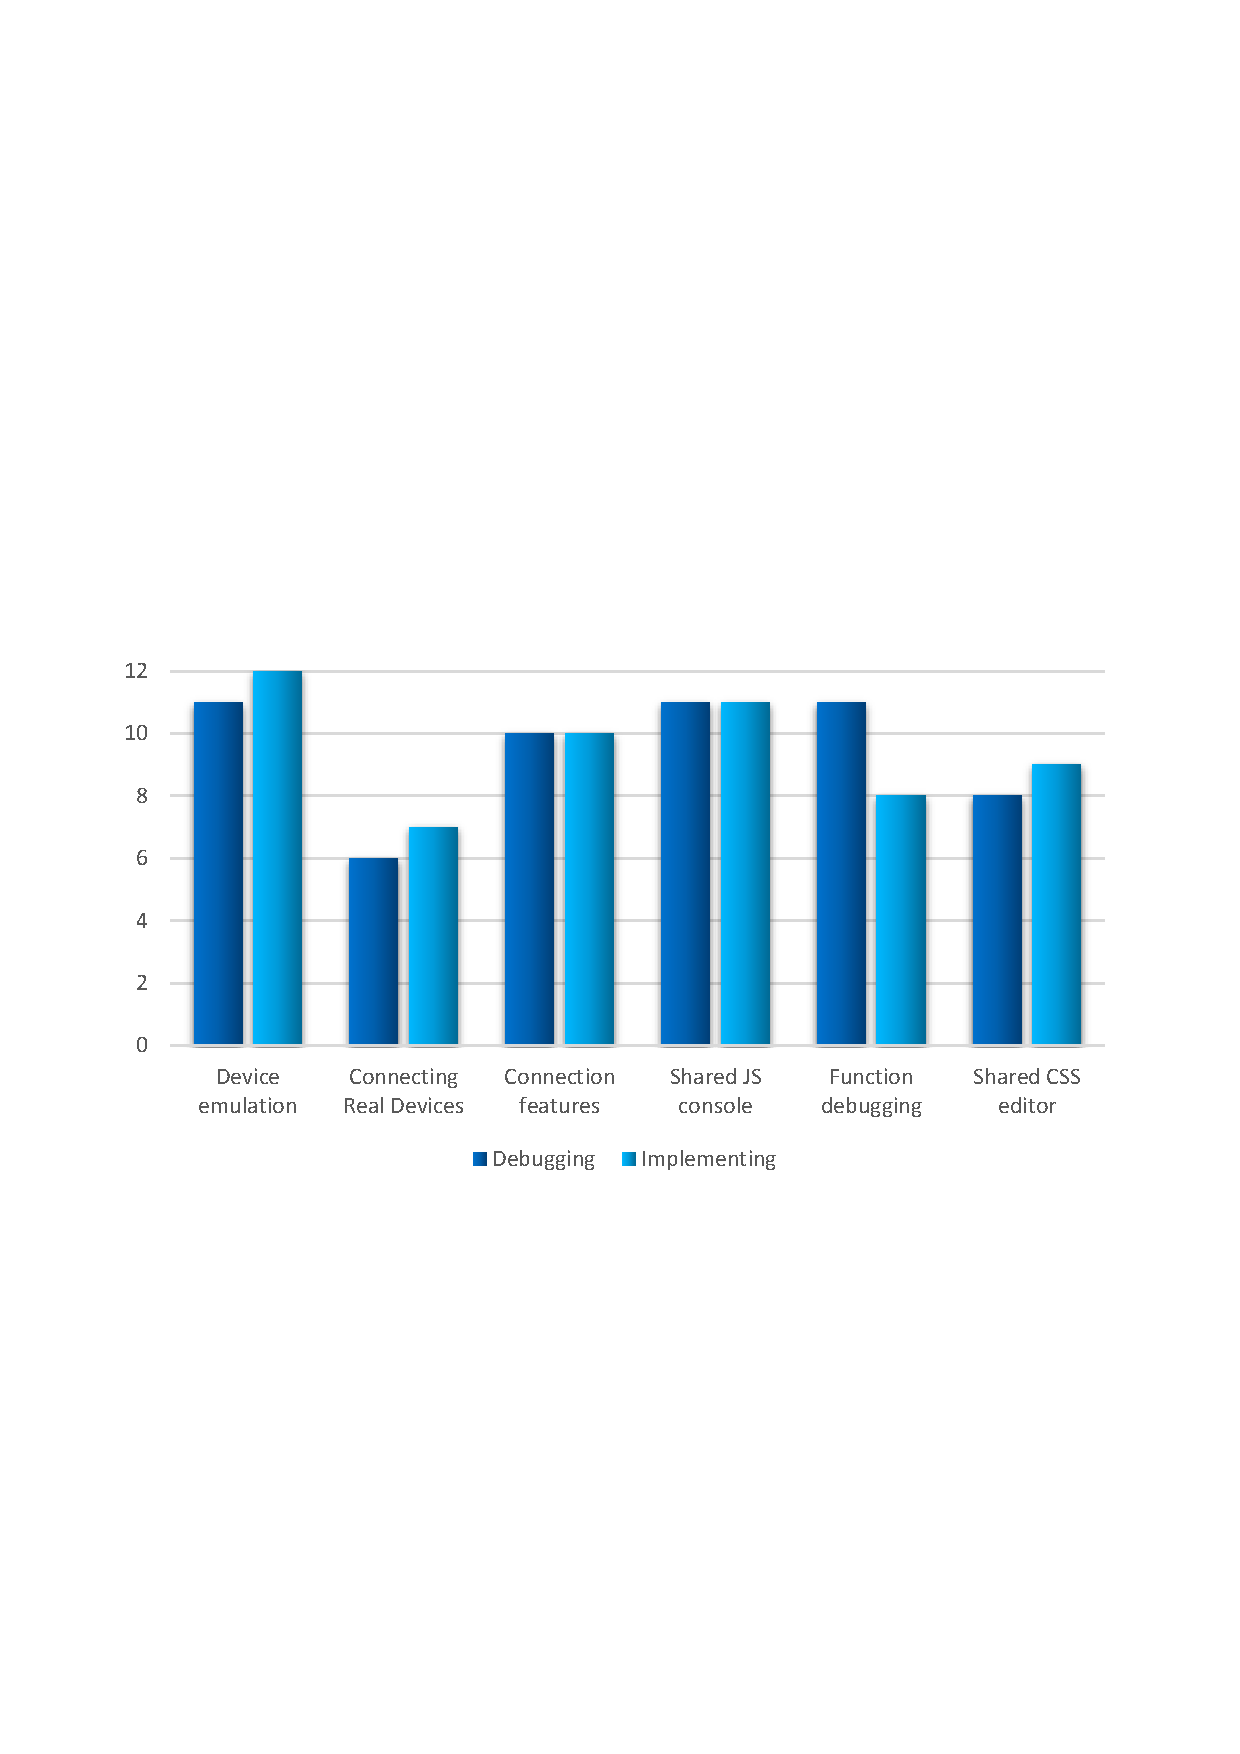
\includegraphics[width=0.8\textwidth]{images/charts/would_use_features.pdf}
	\caption[Features that participants would use]{Features that the participants would use}
	\label{fig:would_use_features}
\end{figure}

During the study, some participants mentioned that they found device emulation very useful because they can have all devices in one place instead of having to manage different browser windows and profiles. Reloading all devices at once was also considered very useful. With multiple browser windows, each window has to be reloaded individually which makes this a much more tedious task. It was also appreciated that the devices are still connected after reloading, though this is also the case with multiple browser windows. The participants really liked function debugging, the only critique was that it does not show on which device a function is called which was fixed after the study. In general, the output aggregation of the shared JavaScript console was considered more useful than sending commands. One participant even mentioned that he would not use it to send commands, but the aggregation is very useful. 

In general, the feedback during the study showed that participants really liked the tool. One participant stated that they think that the tool is very useful and they wish they had access to it when they were working on a cross-device application. Another participant mentioned that "The existing features are already very impressive and work well. They really help the developer working on cross-device applications."

Record/replay was disabled for the user study, but one participant that had attended a presentation about our tools before, mentioned that they would find it immensely useful. They consider it as a powerful feature that could be very helpful for replicating bugs in an application and for regression testing. Often, it is not clear how to reach a bug and being able to record the set of interactions that lead to the bug and then replay them can simplify this process.

\subsubsection{Aborted Tasks}

Due to the time limits that we set, we also had to abort some tasks. There were five cases where we had to abort the task, four while participants had access to our tools, and one where the participant did not have access to our tools. There was one participant that finished all task except the XDCinema debugging task. The participant had access to our tools for this task, but we do not consider this relevant for this specific case, as the time required for completing this task can vary greatly depending on how fast the participant notices the switched variable. Also, the participant had completed all other task successfully. Furthermore, there was one participant for whom we had to abort both implementation tasks (one with our tools and one without) and one participant where we had to abort both XDCinema tasks (both with our tools). Both those participants had very low experience in web application development and had problems completing basic things like placing brackets correctly around an if-statement and creating a new line in HTML. This indicates that those participants had very low programming experience in general and it is not surprising that they failed to complete some tasks. The participants also had problems completing the other tasks, but eventually managed to finish the tasks with a lot of help from the instructor. Thus, we do not think that the fact that most of the aborted tasks were carried out with our tools says anything relevant about our tools. It was simply bad luck that most of the aborted tasks were carried out in this condition.

\subsubsection{Devices Used}

Overall, the number of devices used did not vary greatly depending on the participant and on the condition the participant was in. Although our tasks were designed to require at least two devices in general, it was possible to complete the XDCinema debugging task with only one device, but the task required less device interaction when multiple devices were involved. Figure~\ref{fig:n_emulated} shows how many emulated devices the participants used on average with and without our tools. The number of emulated devices used is slightly higher with our tools for all tasks. One reason for this difference could be that it is easier to add a new device with our tools. However, the difference is rather small and further investigation is needed to see if this is really the case. For the XDCinema debugging task, only two out of six participants that did not have access to our tools used more than one device. With our tools, four participants used more than one device. This also indicates that participants prefer to use more devices when they have access to our tools. For the XDCinema implementation task, all participant used exactly three devices (when combining real and emulated devices) which is not surprising because the minimum number of devices required was three and additional devices did not provide any value. 

\begin{figure}[H]
  \centering
    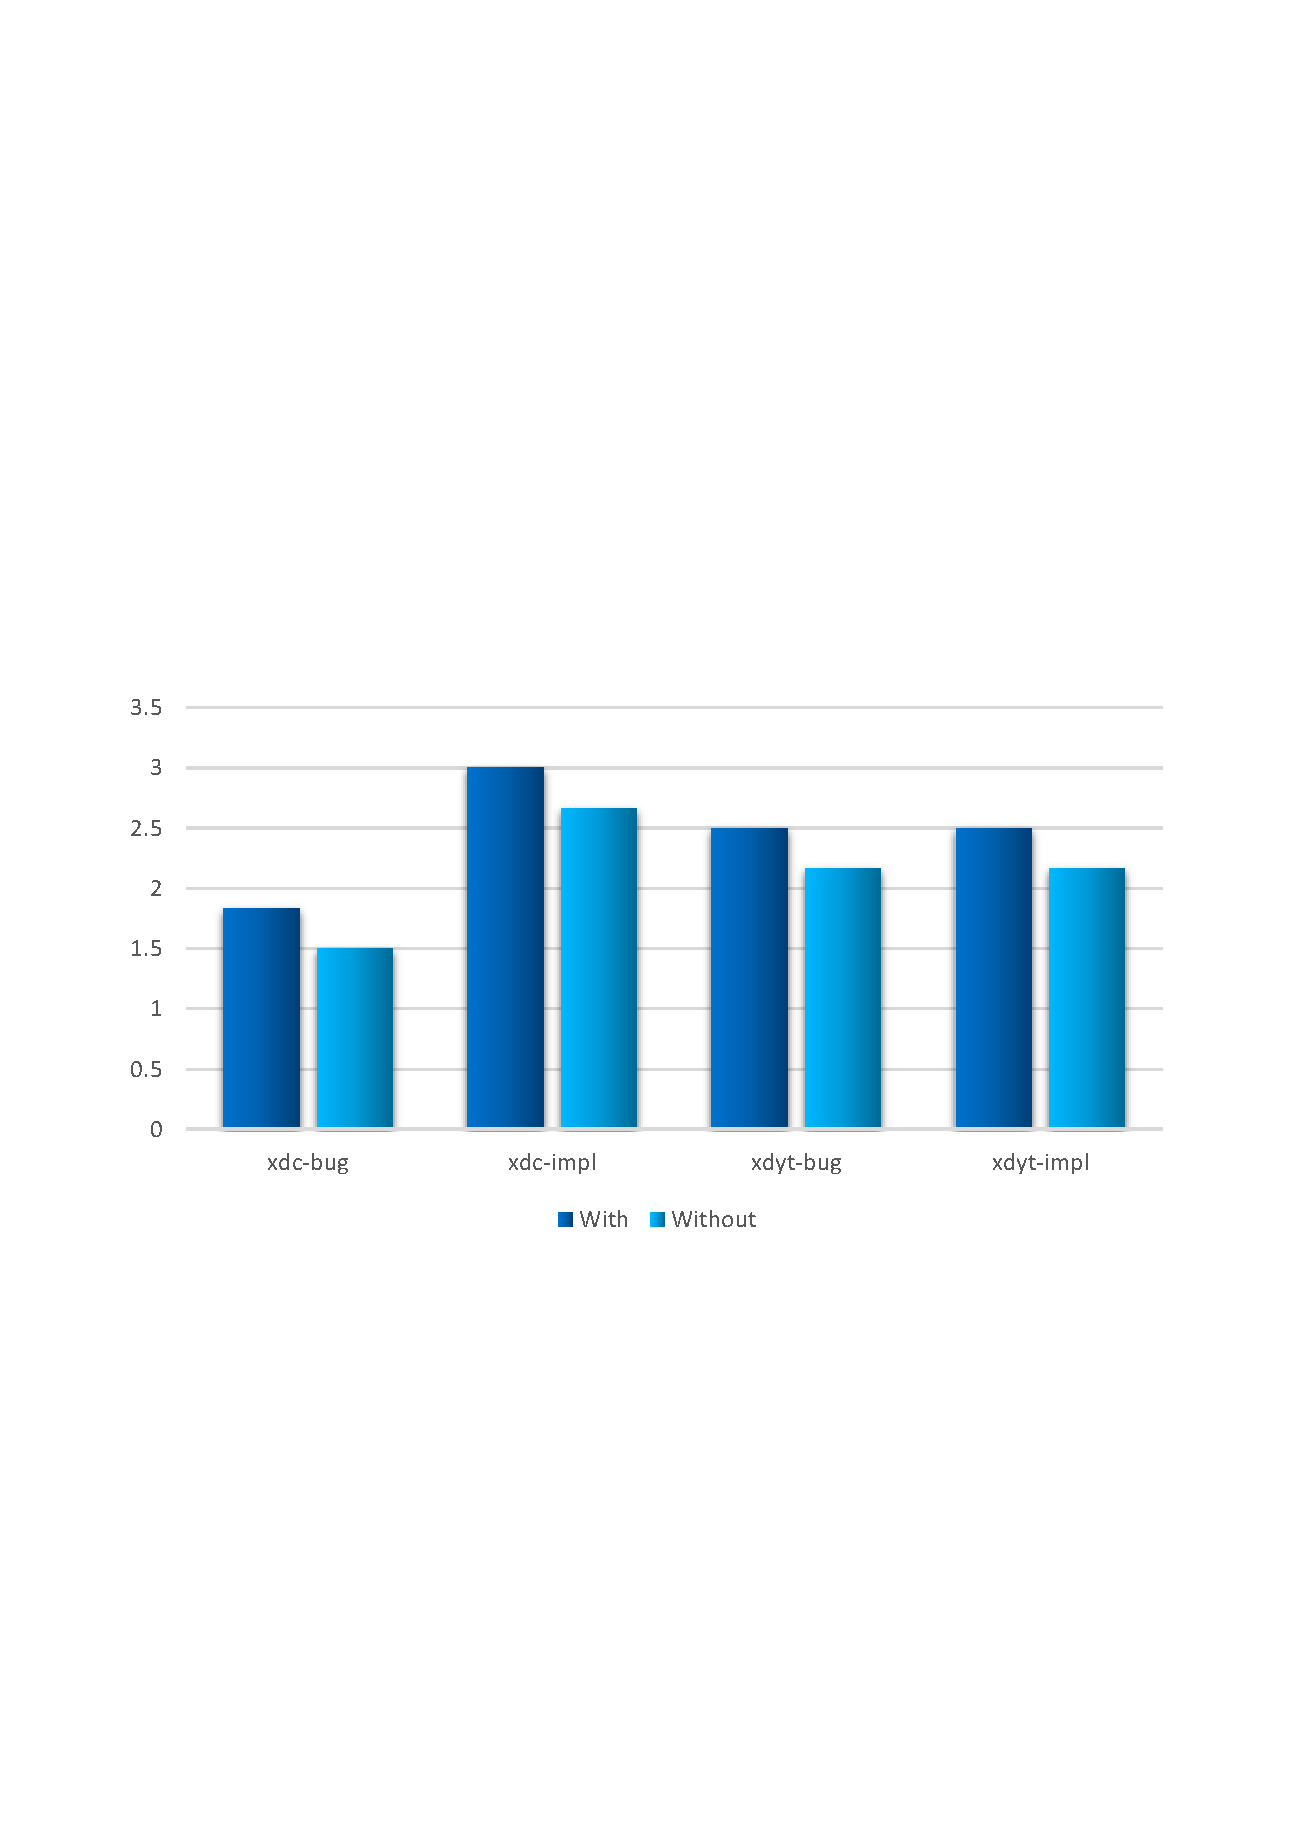
\includegraphics[width=0.8\textwidth]{images/charts/n_emulated.pdf}
	\caption[Emulated device used]{Average number of emulated devices used}
	\label{fig:n_emulated}
\end{figure}

The real devices were only rarely used overall. In the XDYouTube implementation and debugging tasks, one participant per condition used one real device. In the XDCinema implementation task, one participant that did not have access to our tools used two real devices, further supporting our thesis that adding emulated devices is more tedious without access to our tools. Normally, most of the tasks required for implementing cross-device applications can be performed just as well on emulated devices. Testing on real devices is typically limited to points where major implementation steps have been completed or when a developer wants to see how interactions feel or work on actual touch devices. Therefore, it is no surprise that real devices were not used frequently during our study. The number of devices used during the tasks shows that although participants sometimes stick to the minimum number of devices required, they also like to be able to add more devices for convenience of further testing. In the XDYouTube implementation task, participants often added three devices so they could put one in landscape mode and one in portrait mode. This allowed them to add videos to the queue and test their implementation of the remote control button without switching orientation in-between. 

In terms of screen sizes used, participants mostly used low-resolution mobile phones and sometimes tablets when carrying out tasks with our tools. The devices were in portrait mode at almost all times, except for when they were required to be in landscape mode by the application. This is probably due to the dimensions of the area where devices can be placed which makes it more convenient to have devices in portrait mode. Furthermore, most predefined devices are in portrait mode by default and participants did not switch their orientation unless required to. Without access to our tools, participants also often used smaller devices, but sometimes they had one large full-screen browser window and other smaller browser windows that they just switched to when required. Participants that used three devices often let one device fill the left half of the screen and let the other two devices fill one quarter of the screen each, which put them in landscape mode. 

\subsubsection{Debugging/Implementation Strategies}

In both debugging tasks and both conditions, about half the participants started by looking at the code and about half started by trying to reproduce the bug. Most of the participants switched between the code and the application multiple times while carrying out the tasks, although some looked at the code directly in the DevTools. Almost all participants used the DevTools at some point for completing the task, and most of the participants that had access to our tools used function debugging. The debugging task in XDCinema and XDYouTube had some fundamental differences: The main difficulty for the XDYouTube debugging task was reproducing the bug, once the bug was reproduced, the cause of the bug was pretty obvious given the JavaScript error the bug produced. In contrast, reproducing the bug in the XDCinema debugging task was trivial, but finding out what causes the bug is more difficult. In XDYouTube, participants usually spent quite a lot of time trying to reproduce the bug before they switched to the DevTools or function debugging. Only after participants failed at reproducing the bug, they used tools for debugging in an attempt to find the bug in this way. In XDCinema, participants switched to the DevTools or function debugging much faster because they reproduced the bug almost immediately. Consequently, in XDYouTube, much more time is spent switching between the code and application because the participants try out different ways of finding the bug. In XDCinema, the debugging process is much more streamlined because after reproducing the bug, participants mostly stick to either looking at the code or using tools for debugging.

In the implementation task, some participants started by looking for the HTML-element that contained the prices or the remote control button first, while others started implementing right away. All participants implemented everything required for the XDYouTube implementation task at once and only then started testing it. Only the CSS was usually added after making sure that the button works. On one hand, it makes sense to implement the complete remote control functionality at once because if only part of it was implemented, it would be difficult to see if the implemented function actually works. On the other hand, we would have expected that at least some participants implemented part of the functionality and used logging mechanisms to see if it works. In the XDCinema implementation task, the task was clearly separated into to parts and the first part did not require the second part to work. Thus, all except one participant implemented the first part, tested it, and then moved on to the second part. However, almost all participants had to modify their first part a little bit while implementing the second part because of the different requirements. The CSS part of the task was again implemented after completing everything else by most participants.

In summary, no real difference in implementation and debugging strategies can be seen between the two conditions of our study. The only difference is that some parts of the debugging process are made more efficient or easier because the developer has access to additional tools. Thus, developers should be able to use the same strategies for debugging and implementing features as they usually would and augment them with additional features where it is useful. 

\subsubsection{Feature Requests}

During the study, some participants suggested some improvements to existing features that would help them even more. Multiple participants suggested that function debugging should show on which device a function is called. We were able to successfully implement this feature after completing the user study. Also, one participant said that auto-connect should be enabled by default because there rarely is a situation where a developer would not want to connect the devices. Over the course of the study, it became obvious that this feature would be useful because many participants forgot to enable auto-connect before adding more devices and thus either manually connected them or removed them, enabled auto-connect, and re-added the devices. Furthermore, it was suggested that the border of the device should be in the device's unique color so devices can more easily be recognized. Those two features were also included into our tools after the study. Also, it became clear during the study that it was not at all obvious when function debugging was working and when the participants had to re-open the DevTools. Due to this, we now show a warning when the developer should re-open the DevTools to make sure that function debugging works. Also, we now display a warning message when the user wants to reload the page because many participants accidentally reload the page instead of the devices and then lose all their devices. Some additional feature suggestions include:
\begin{itemize}
	\item CSS value suggestions, e.g. suggest "1px solid black" when the developer sets the border property
	\item More integration with the DevTools
	\item Opening the DevTools automatically when the developer wants to debug a function
	\item Auto-complete or similar for functions in function debugging
	\item Combining a source code editor with our tools
\end{itemize}
Due to time constraints and in some cases also feasibility constraints we were not able to implement those feature requests (yet). Also, while some of those requests like CSS value suggestions would clearly be useful, others like combining a source code editor with our tools require more research to determine if they are actually desired by developers and would provide some additional benefits.
\section{Future Work}

Extended record and replay: Record things like dates, server responses, random numbers, ...

Extended device emulation: Network, location, touch, ...

Tighter integration with debugging tools or browser

Long-term study: Let participants use and evaluate tools over longer period of time

\appendix

\chapter{Questionnaires}
\label{sec:questionnaires}
\newpage
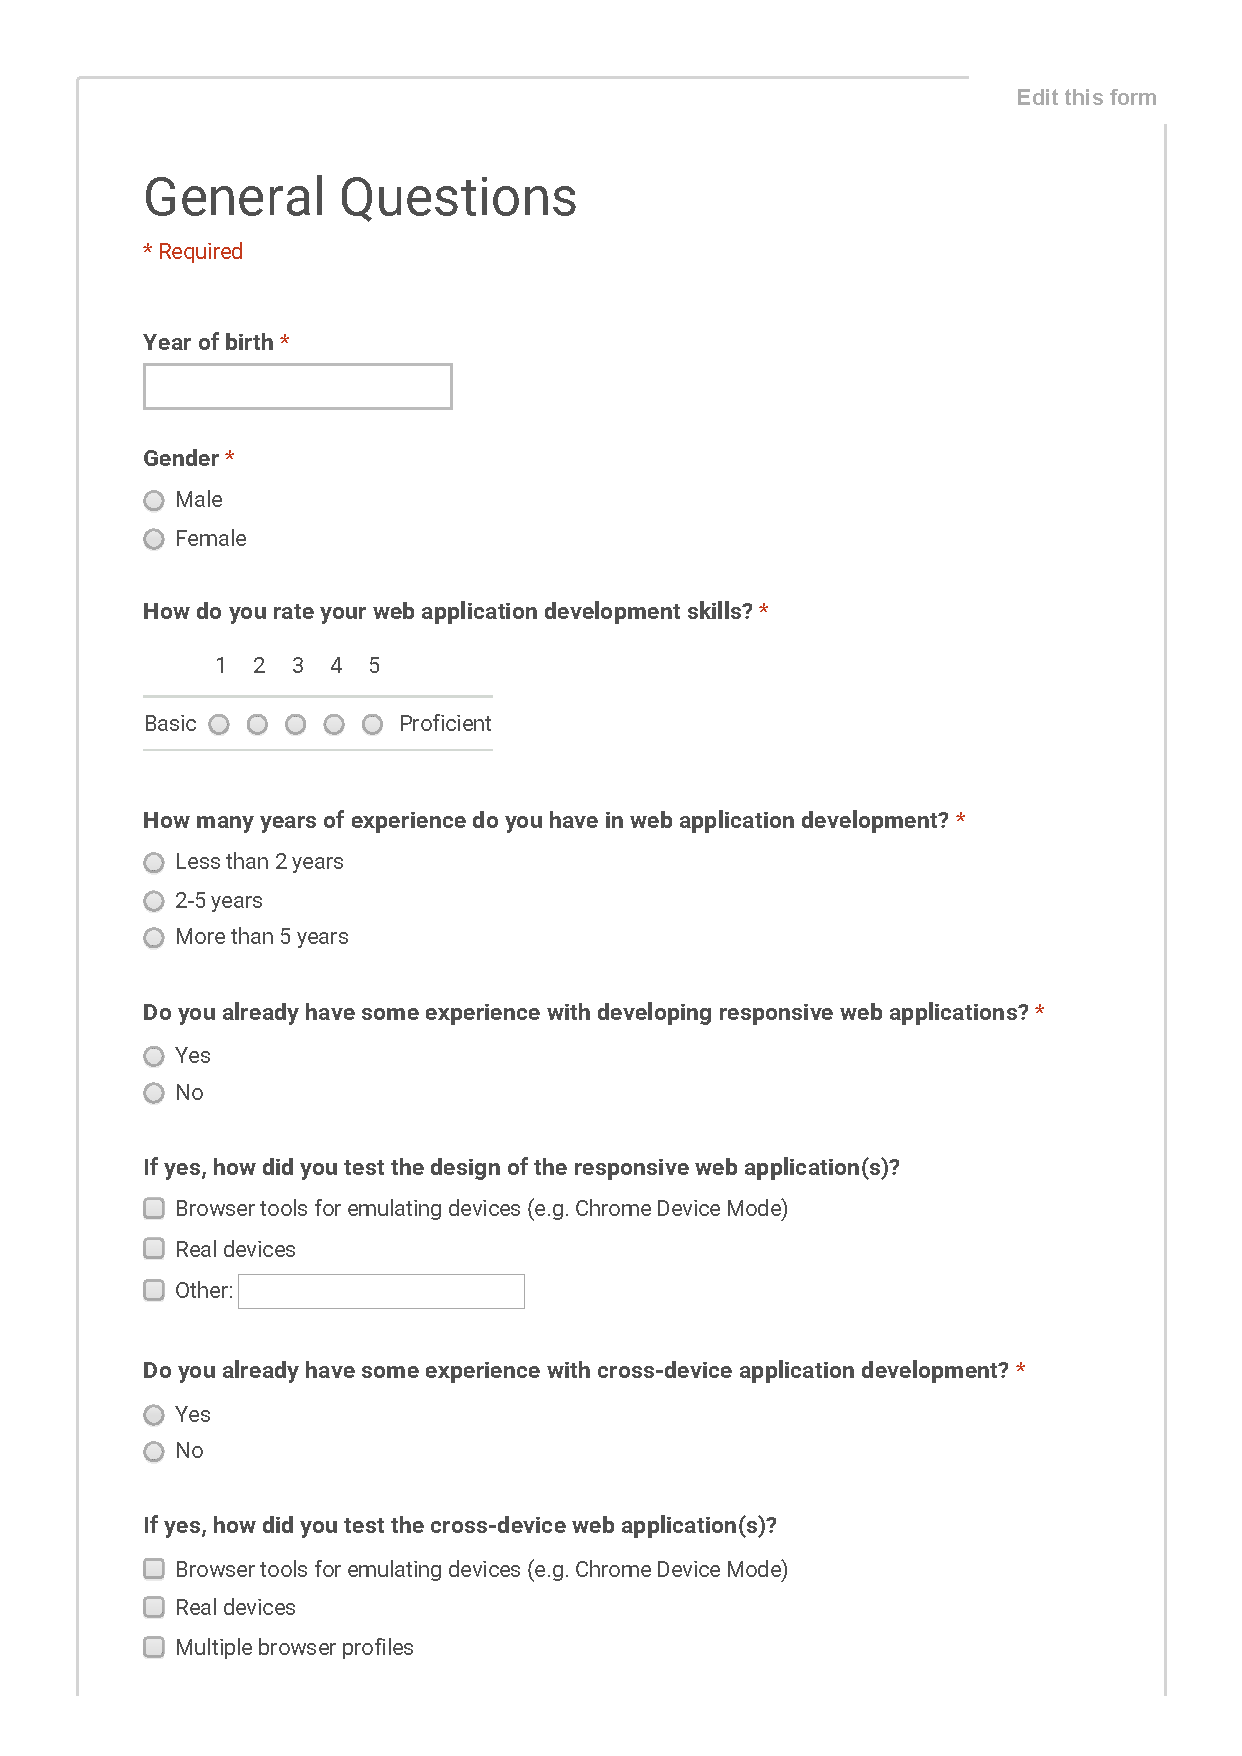
\includepdf[pages={1-}]{appendix/questionnaires/general_2.pdf}
\newpage
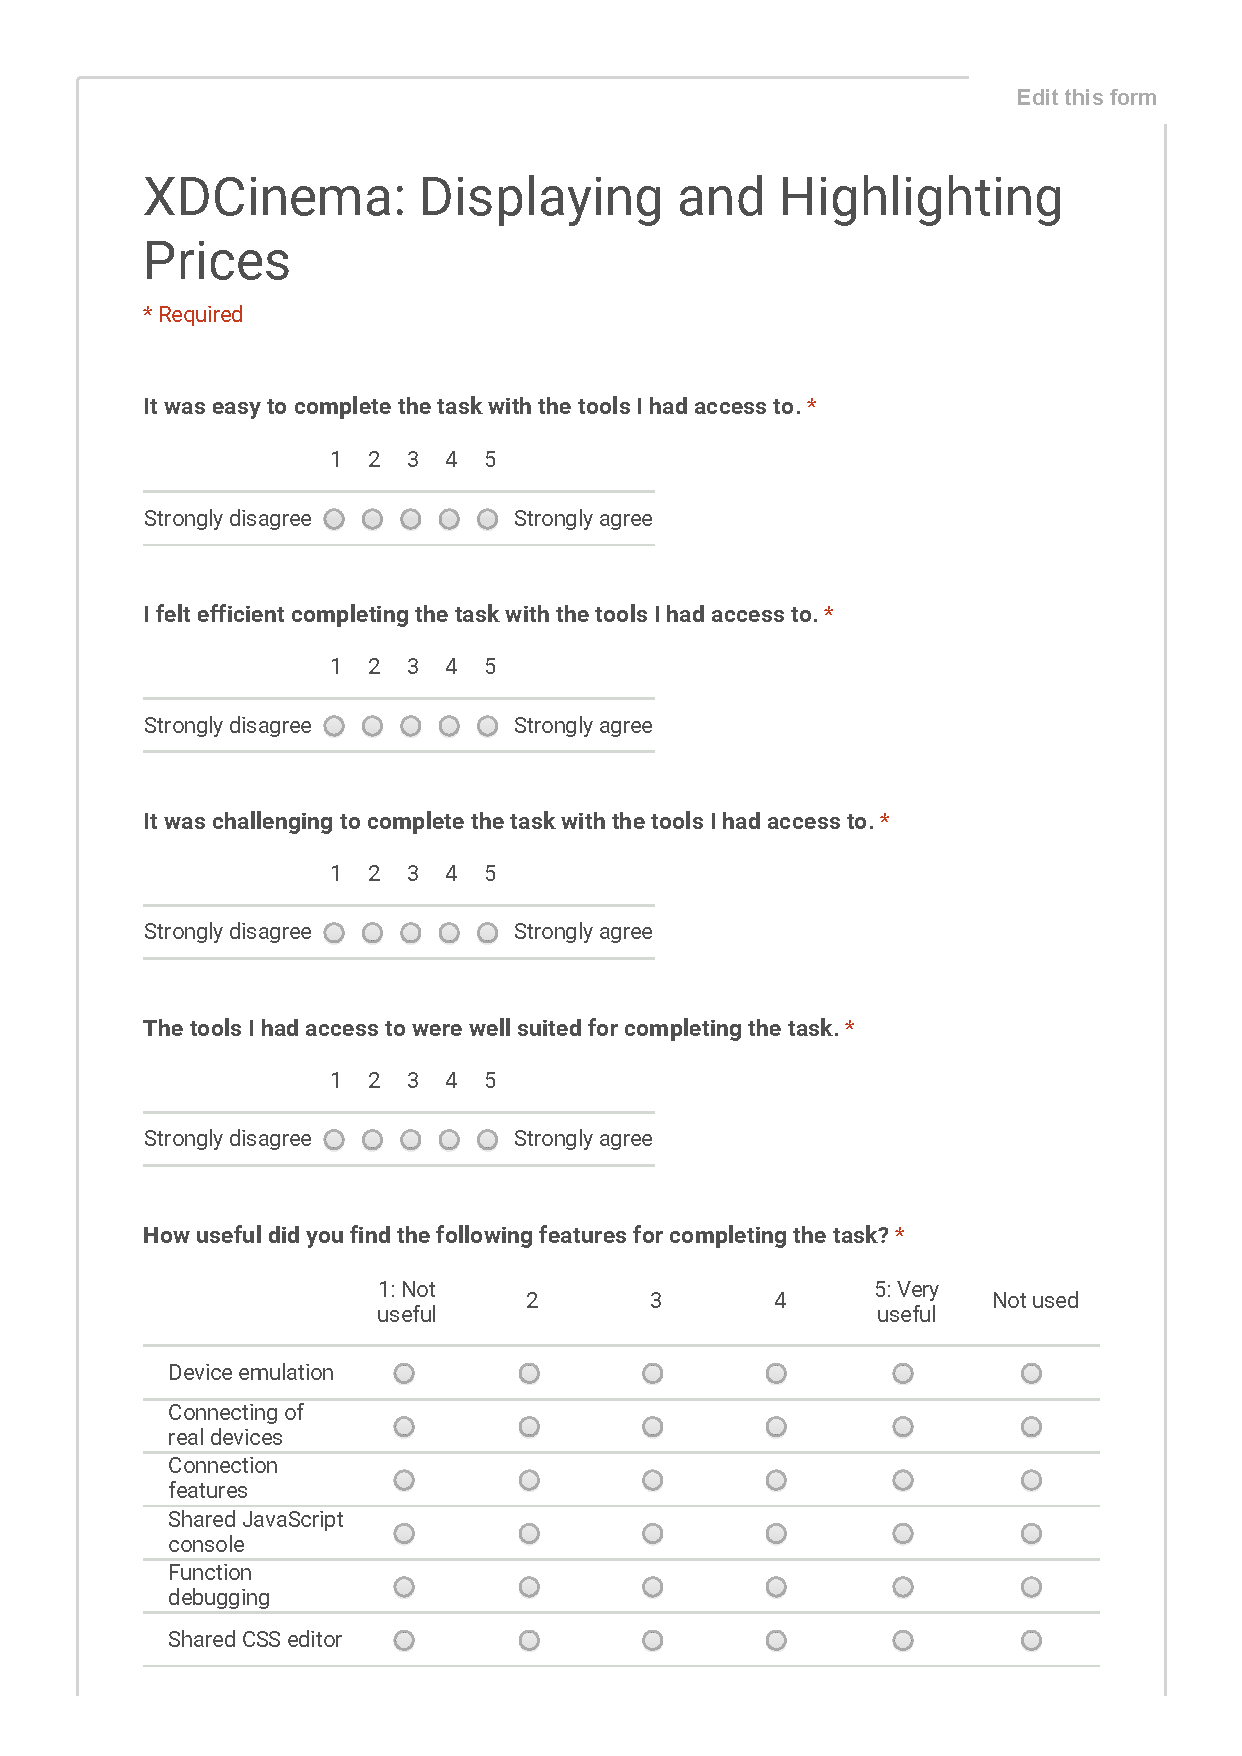
\includepdf[pages={1-}]{appendix/questionnaires/with_tools_2.pdf}
\newpage
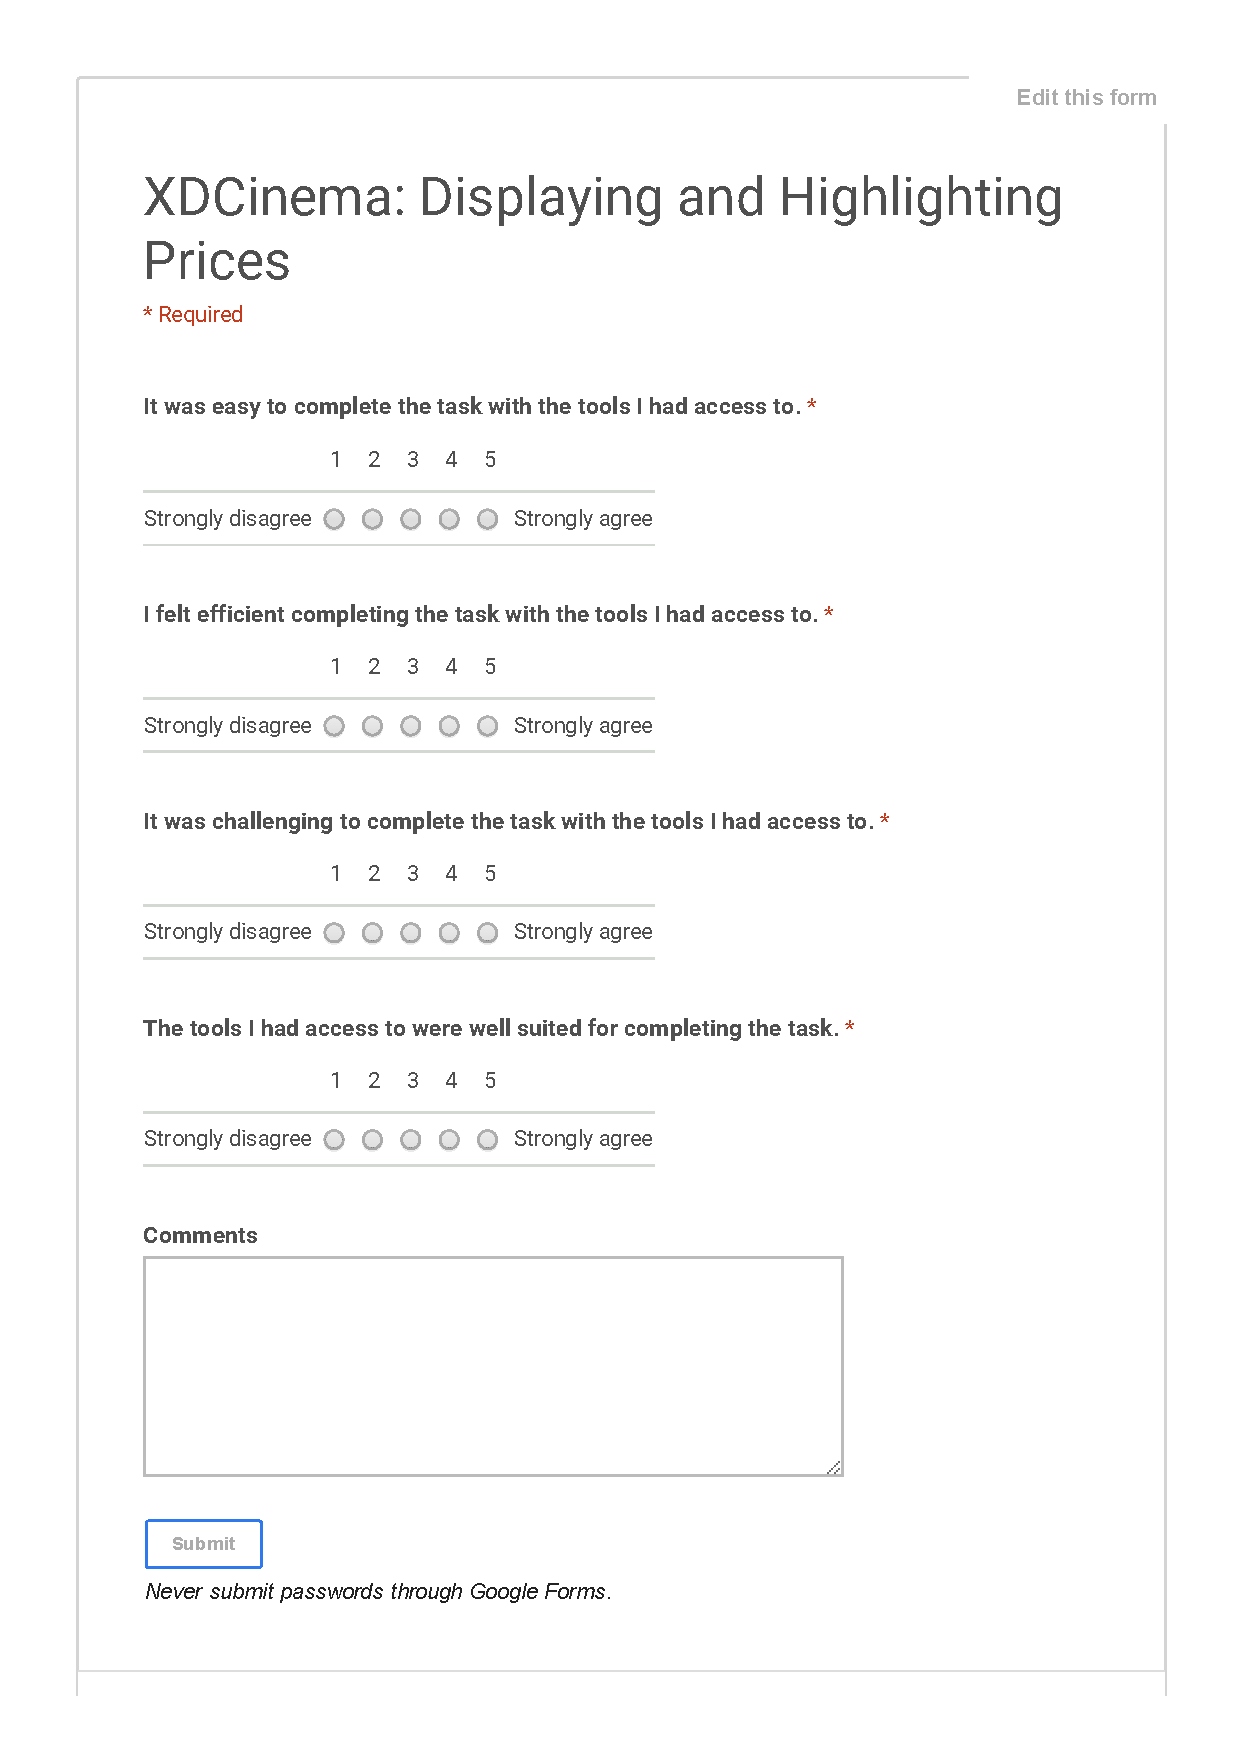
\includepdf[pages={1-}]{appendix/questionnaires/without_tools_2.pdf}
\newpage
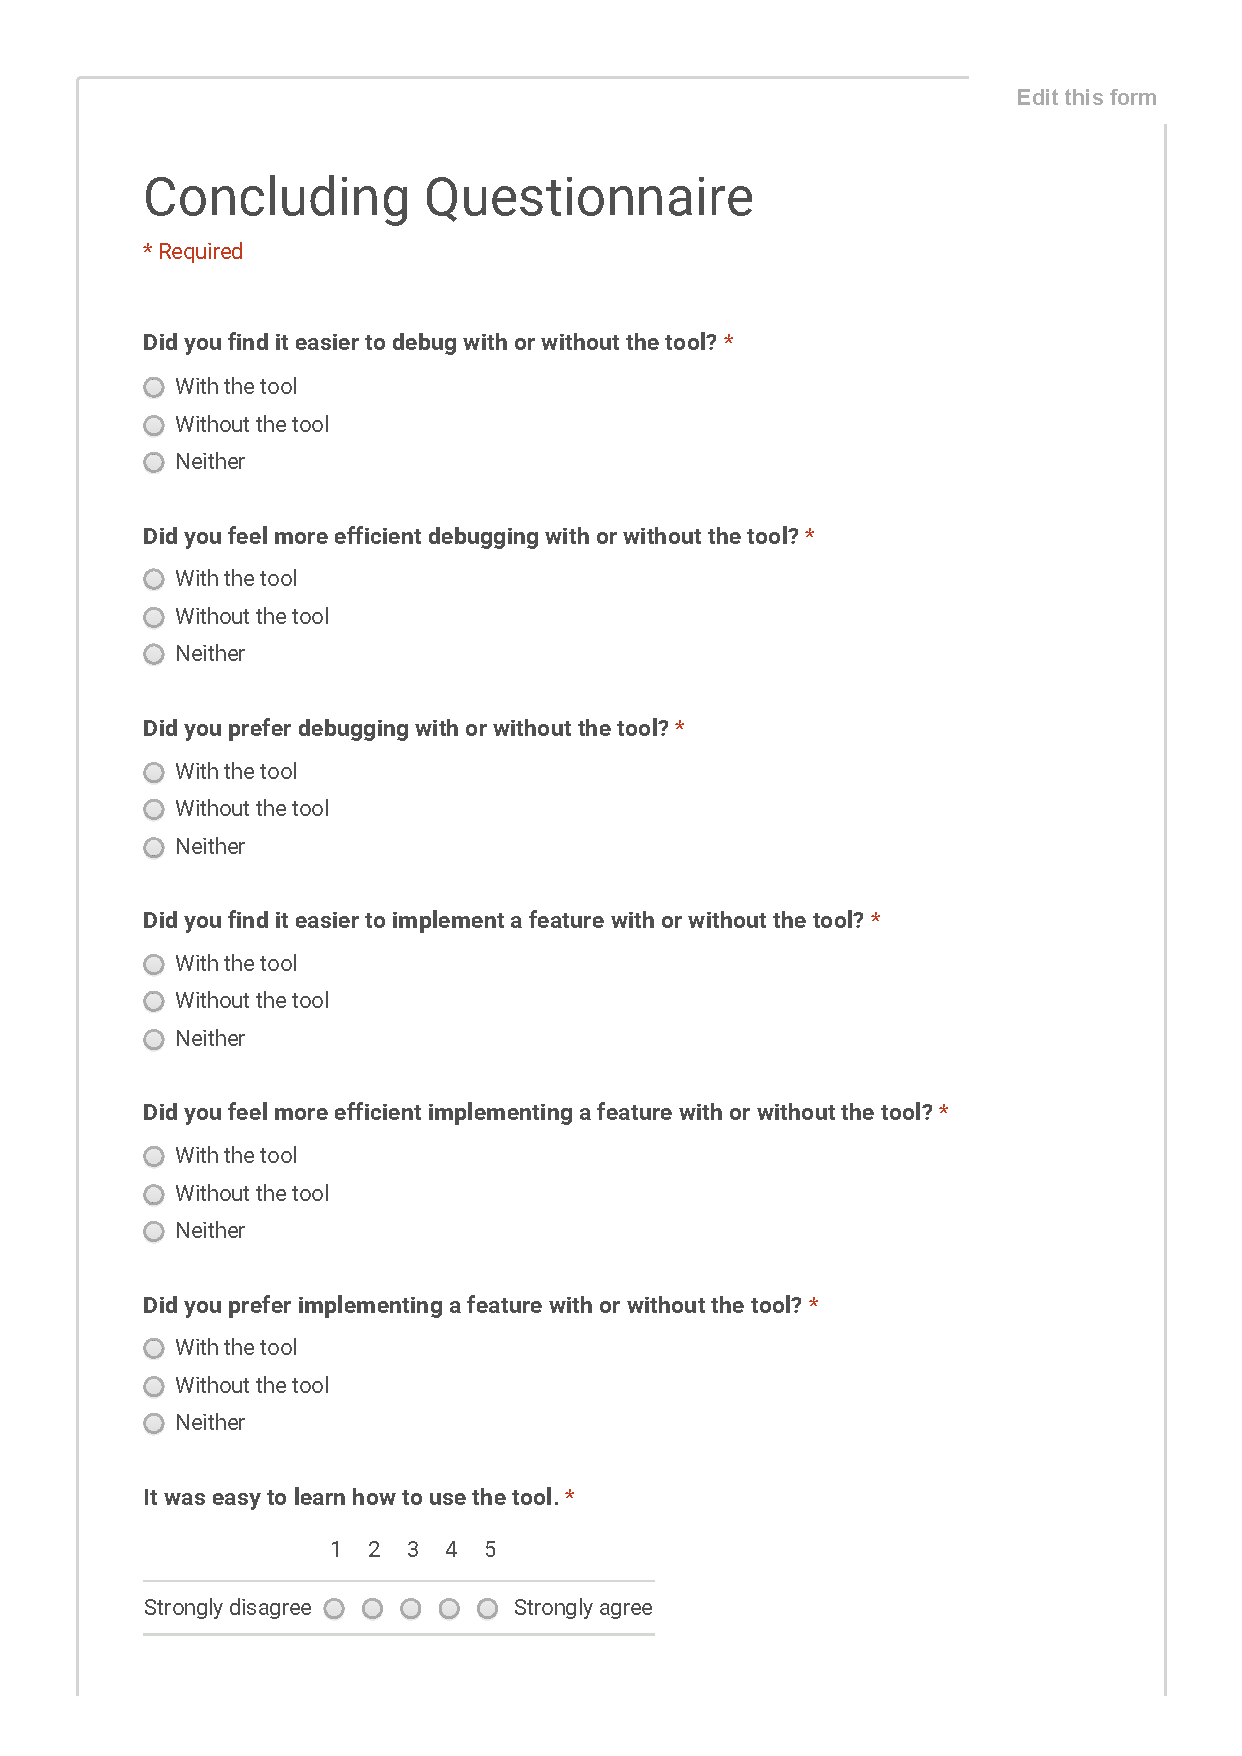
\includepdf[pages={1-}]{appendix/questionnaires/concluding_2.pdf}

\chapter{Tasks}
\label{sec:tasks}
\newpage
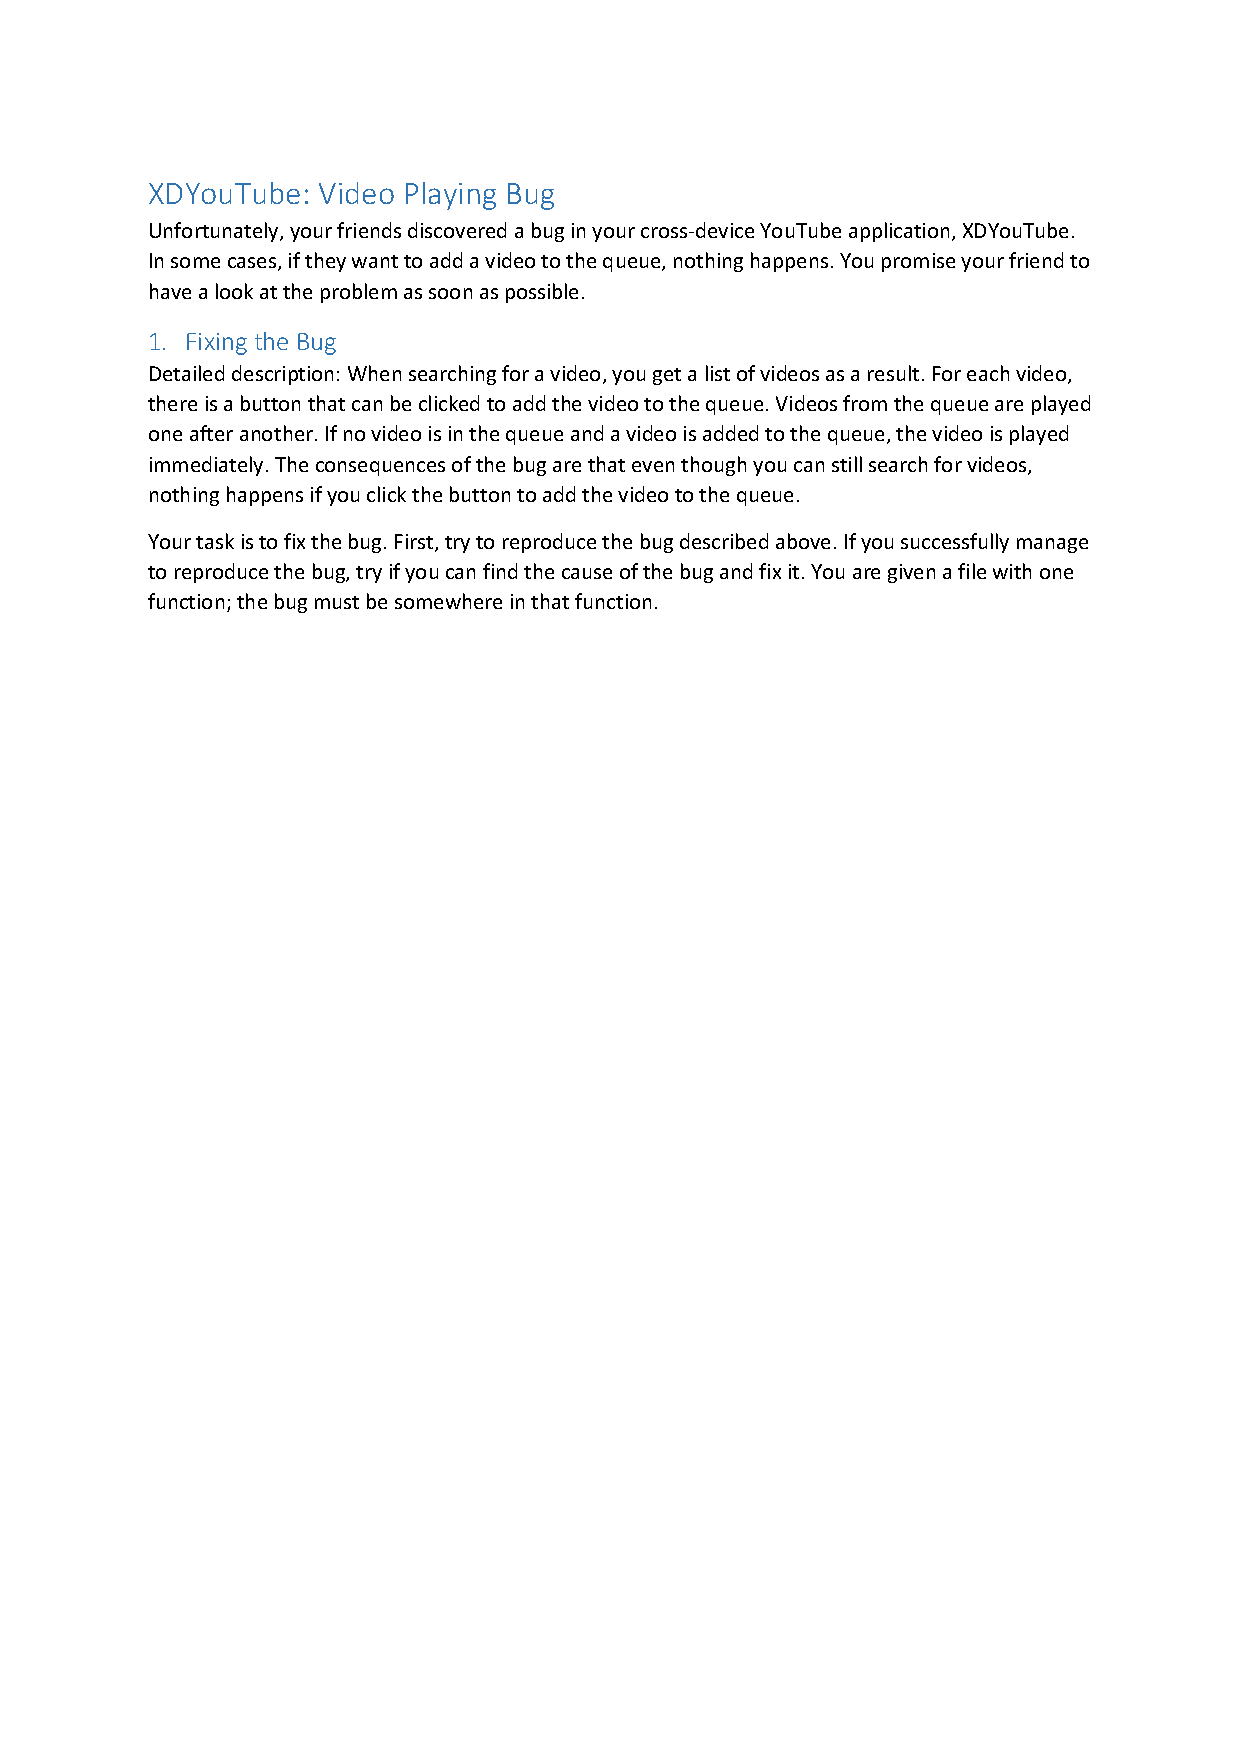
\includepdf[pages={1-}]{appendix/tasks/xdyt-bug.pdf}
\newpage
\includepdf[pages={1-}]{appendix/tasks/xdyt-impl.pdf}
\newpage
\includepdf[pages={1-}]{appendix/tasks/xdc-bug.pdf}
\newpage
\includepdf[pages={1-}]{appendix/tasks/xdc-impl.pdf}


\listoffigures
\listoftables

\chapter*{Acknowledgements}

TODO

\newpage
\thispagestyle{empty}

\bibliographystyle{plain}
\bibliography{bibliography}

\end{document} 
